%==============================================================================
% ETHASL - Template for student projects at the ASL
% 2013.10: Péter Fankhauser
% This template is based on the IMRT Latex template by Eric A. Mueller.
%==============================================================================

\documentclass[10pt,twoside,a4paper]{report}

% ETHASL package
% TODO Choose options according to your project
% som/bt/st/mt: Studies on Mechatronics, Bachelor Thesis, Semester Thesis, Master Thesis
% fs/hs: Spring term, Autumn term
% german/english: German/English
\usepackage[st,hs,english]{packages/ethrsl}

% Activate for german language
%\usepackage{german}
%\usepackage{ae}

%%%%%%%%%%%%%%%%%%%%%%%%%%%%%%%%%%%%%%%%%%%%%%%%%%%%%%%%%%%%%%%%%%%%%%%%%%%%%%%
% LaTeX preamble
%%%%%%%%%%%%%%%%%%%%%%%%%%%%%%%%%%%%%%%%%%%%%%%%%%%%%%%%%%%%%%%%%%%%%%%%%%%%%%%
% Encoding settings
\usepackage[utf8]{inputenc}
\usepackage[OT1]{fontenc}

% Paper size
\usepackage{a4}

% Headings
\usepackage{fancyhdr}

% More symbols
\usepackage{textcomp}\usepackage{gensymb}

% Math support for Times font
%\usepackage{txfonts}

% ISO date
\usepackage[english]{isodate}

% Multi column
\usepackage{multicol}

% Figures
\usepackage{graphicx}

% Subfigures (obsolete)
% \usepackage{subfigure}
\usepackage{subfig}

% Bibliography
\usepackage[numbers]{natbib}

% Nicer tables
\usepackage{booktabs}
\usepackage{array}
\usepackage{multirow}
\usepackage{enumitem}
\usepackage{makecell}

% Colors
\usepackage{color}
\usepackage{colortbl}
\definecolor{black}{rgb}{0,0,0}
\definecolor{white}{rgb}{1,1,1}
\definecolor{darkred}{rgb}{0.5,0,0}
\definecolor{darkgreen}{rgb}{0,0.5,0}
\definecolor{darkblue}{rgb}{0,0,0.5}
\usepackage[dvipsnames]{xcolor}

% Additional math functionality
\usepackage{amsmath}
\usepackage{amssymb}

% Nice fractions
\usepackage{nicefrac}

% Upper case greek letters
\usepackage{upgreek}

% ISO math notation
\usepackage{isomath}
\renewcommand{\vec}{\vectorsym}
\newcommand{\mat}{\matrixsym}

% Units
\usepackage{units}

%special signs
\usepackage{lmodern,textcomp}

% Rotated objects
\usepackage{rotating}

% Indent
\setlength{\parindent}{0em}

% Include PDF pages
\usepackage{pdfpages}
\includepdfset{pages={-}, frame=true, pagecommand={\thispagestyle{fancy}}}

% Headings
\rhead[\thepage]{\nouppercase{\rightmark}}
\lhead[\nouppercase{\leftmark}]{\thepage}
\cfoot{}

% Gantt chart
\usepackage{pgfgantt}

% Links (last package)
\PassOptionsToPackage{hyphens}{url}\usepackage{hyperref}

% Clever references (has to be loaded after hyperref)
\usepackage{cleveref}


%%%%%%%%%%%%%%%%%%%%%%%%%%%%%%%%%%%%%%%%%%%%%%%%%%%%%%%%%%%%%%%%%%%%%%%%%%%%%%%
% Title page
%%%%%%%%%%%%%%%%%%%%%%%%%%%%%%%%%%%%%%%%%%%%%%%%%%%%%%%%%%%%%%%%%%%%%%%%%%%%%%%
\begin{document}

% TODO Add your title
\title{Handheld Augmented Reality for Robotic Excavators}
%\subtitle{bla bla bla}

% TODO Add name of the authors
\studentA{Lasse Fierz}

% \studentC{Student 3}

% TODO Add name of the supervisors
\supervisionA{Dominic Jud}
\supervisionB{Ryan Luke Johns}
% \supervisionC{Supervisor C}

% TODO Change if necessary
\projectYear{\the\year} % This year
%\projectYear{\advance\year by -1 \the\year\advance\year by 1} % Last year

\maketitle
\pagestyle{plain}
\pagenumbering{roman}

%%%%%%%%%%%%%%%%%%%%%%%%%%%%%%%%%%%%%%%%%%%%%%%%%%%%%%%%%%%%%%%%%%%%%%%%%%%%%%%
% Declaration of originality
%%%%%%%%%%%%%%%%%%%%%%%%%%%%%%%%%%%%%%%%%%%%%%%%%%%%%%%%%%%%%%%%%%%%%%%%%%%%%%%
\pagestyle{empty}

% TODO Modify placeholders in declaration.tex
% % TODO Add title, student first/last name, supervisor first/last name.

\section{Declaration of Originality}

\vspace{0.5cm}

I hereby declare that the written work I have submitted entitled

\vspace{0.5cm}

% TODO Add title
\textbf{Robot Localization using Visual Features on LiDAR Data}

\vspace{0.5cm}

is original work which I alone have authored and which is written in my own words.\footnote{Co-authored work: The signatures of all authors are required. Each signature attests to the originality of the entire piece of written work in its final form.}

\vspace{1cm}

\textbf{Author(s)}

\vspace{0.5cm}

\begin{tabular}{ p{5cm} p{5cm} }
% TODO Add student first/last name
  Lasse & Fierz \\
\end{tabular}

\vspace{0.5cm}

\textbf{Student supervisor(s)}

\vspace{0.5cm}

\begin{tabular}{ p{5cm} p{5cm} }
% TODO Add supervisor first/last name
  Julian & Nubert \vspace{5mm}\\
  Shehryar & Khattak\\
\end{tabular}

\vspace{0.5cm}

\textbf{Committee members(s)}

\vspace{0.5cm}

\begin{tabular}{ p{5cm} p{5cm} }
  % TODO Add committee member first/last name
  Edo & Jelavic \vspace{0.5cm} \\
  Alexander & Reske\\
\end{tabular}

\vspace{0.5cm}

\textbf{Supervising lecturer}

\vspace{0.5cm}

\begin{tabular}{ p{5cm} p{5cm} }
  Marco & Hutter \\
\end{tabular}

\vspace{1cm}

With the signature I declare that I have been informed regarding normal academic citation rules and that I have read and understood the information on `Citation etiquette' (\url{https://www.ethz.ch/content/dam/ethz/main/education/rechtliches-abschluesse/leistungskontrollen/plagiarism-citationetiquette.pdf}).
The citation conventions usual to the discipline in question here have been respected.

\vspace{0.5cm}

The above written work may be tested electronically for plagiarism.

\vspace{4cm}

\begin{tabular}{ p{5cm} p{1cm} p{5cm} }
  \cline{1-1} \cline{3-3}
  Place and date & & Signature \\
\end{tabular}

% \clearpage
% % TODO Add title, student first/last name, supervisor first/last name.

\section{Intellectual Property Agreement}

%\vspace{1cm}
%\subsection{Preamble}

The student acted under the supervision of Prof. Hutter and contributed to research of his group.
Research results of students outside the scope of an employment contract with ETH Zurich belong to the students themselves.
The results of the student within the present thesis shall be exploited by ETH Zurich, possibly together with results of other contributors in the same field.
To facilitate and to enable a common exploitation of all combined research results, the student hereby assigns his rights to the research results to ETH Zurich.
In exchange, the student shall be treated like an employee of ETH Zurich with respect to any income generated due to the research results.

This agreement regulates the rights to the created research results.



\subsubsection{1. Intellectual Property Rights} 

\begin{enumerate}[topsep=0pt,itemsep=0ex,partopsep=1ex,parsep=1ex]
\item The student assigns his/her rights to the research results, including inventions and works protected by copyright, but not including his moral rights (“Urheberpers\"onlichkeitsrechte”), to ETH Zurich. Herewith, he cedes, in particular, all rights for commercial exploitations of research results to ETH Zurich. He is doing this voluntarily and with full awareness, in order to facilitate the commercial exploitation of the created Research Results. The student's moral rights (“Urheberpers\"onlichkeitsrechte”) shall not be affected by this assignment.

\item	In exchange, the student will be compensated by ETH Zurich in the case of income through the commercial exploitation of research results. Compensation will be made as if the student was an employee of ETH Zurich and according to the guidelines  \href{https://rechtssammlung.sp.ethz.ch/Dokumente/440.4.pdf?Web=1}{“Richtlinien f\"ur die wirtschaftliche Verwertung von Forschungsergebnissen der ETH Z\"urich”}.

\item	The student agrees to keep all research results confidential. This obligation to confidentiality shall persist until he or she is informed by ETH Zurich that the intellectual property rights to the research results have been protected through patent applications or other adequate measures or that no protection is sought, but not longer than 12 months after the collaborator has signed this agreement.

\item If a patent application is filed for an invention based on the research results, the student will duly provide all necessary signatures. He/she also agrees to be available whenever his aid is necessary in the course of the patent application process, e.g. to respond to questions of patent examiners or the like. 

\end{enumerate}

\subsubsection{2. Settlement of Disagreements}

Should disagreements arise out between the parties, the parties will make an effort to settle them between them in good faith.
In case of failure of these agreements, Swiss Law shall be applied and the Courts of Zurich shall have exclusive jurisdiction.



\vspace{3cm}

\begin{tabular}{ p{5cm} p{1cm} p{5cm} }
  \cline{1-1} \cline{3-3}
  Place and date & & Signature \\
\end{tabular}

\begin{center}
    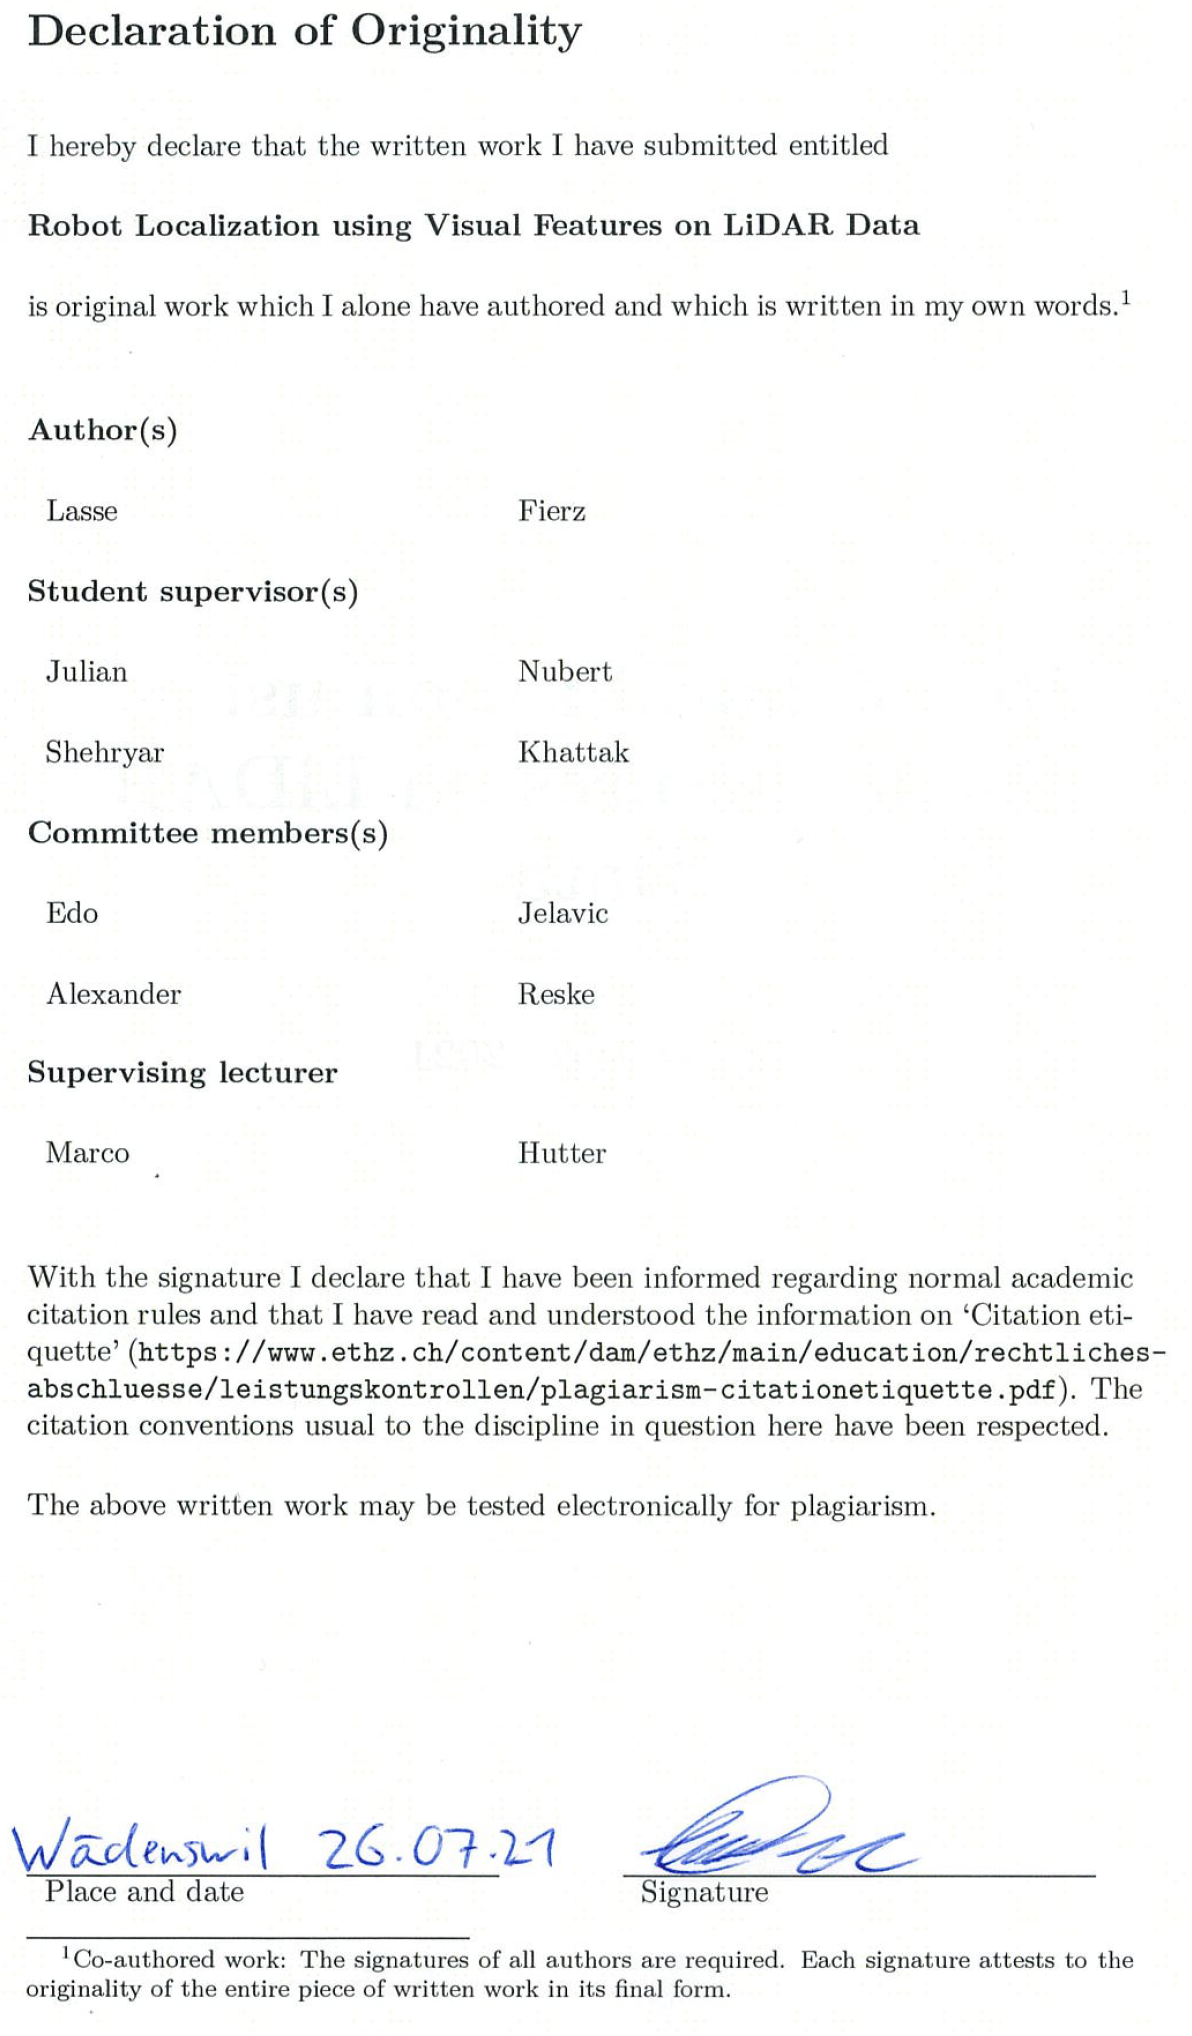
\includegraphics[scale=0.65]{images/declaration/or_rep.png}
    
\includegraphics[scale=0.65]{images/declaration/prop.png}
\end{center}
%%%%%%%%%%%%%%%%%%%%%%%%%%%%%%%%%%%%%%%%%%%%%%%%%%%%%%%%%%%%%%%%%%%%%%%%%%%%%%%
% Table on contents
%%%%%%%%%%%%%%%%%%%%%%%%%%%%%%%%%%%%%%%%%%%%%%%%%%%%%%%%%%%%%%%%%%%%%%%%%%%%%%%

% Table of Contents depth (TODO change if necessary)
\setcounter{tocdepth}{2}

\cleardoublepage
\tableofcontents

%%%%%%%%%%%%%%%%%%%%%%%%%%%%%%%%%%%%%%%%%%%%%%%%%%%%%%%%%%%%%%%%%%%%%%%%%%%%%%%
% Chapters standard
%%%%%%%%%%%%%%%%%%%%%%%%%%%%%%%%%%%%%%%%%%%%%%%%%%%%%%%%%%%%%%%%%%%%%%%%%%%%%%%
\chapter*{Preface}
\addcontentsline{toc}{chapter}{Preface}

The aspiration for this project was to contribute to the process of making use of new technology in order to assist humankind. The field of robotics has tremendous potential in this regard and I feel fortunate to be partaking in this endeavour.
\clearpage
\chapter{Abstract}


This project aimed at paving the way for the creation of a high level remote control for autonomous excavators using a handheld augmented reality device. 

The two key requirements for such an endeavour are first of all to be able to send data as well as inputs back and forth between the two devices. Secondly there are two camera views in this setup the AR view of the handheld device and the image input that the excavator receives. In order to precisely send geometric inputs from one device to the other colocalization is required. 

The idea was to connect the handheld device and the excavator through an Unreal Engine multiplayer connection as an Unreal Engine setup was already implemented on the excavator. For the colocalization requirement the idea was to make use of the possibilities that come through the AR setup. In this case Microsoft's Azure Spatial Anchors which allow for a very simple colocalization implementation.

These methods were chosen to solve a specific task however it is also interesting to observe how these technologies that are less conventional in the robotic world interact with a robotic system.

% The idea was to connect the handheld device making use of Unreal Engine game instances. For the excavator's side this was already setup. For the colocalization requirement the approach was to use Microsoft's Azure Spatial Anchors for a frictionless implementation between the two camera origins. Thus an additional goal was to further understand the capabilities of these less conventional methods for robotic applications.
\clearpage
% \chapter{Symbols}
\label{sec:symbols}
\addcontentsline{toc}{chapter}{Symbols}
%\chapter{Symbolverzeichnis}
%\label{sec:symbole}
%\addcontentsline{toc}{chapter}{Symbolverzeichnis}

\section{Symbols}
%\section{Symbole}

\begin{tabbing}
 \hspace*{1.6cm} \= \kill
  $\phi, \theta, \psi$    \> roll, pitch and yaw angle \\[0.5ex] 					
  $b$                     \> gyroscope bias \\[0.5ex]										
  $\Omega_m$              \> 3-axis gyroscope measurement \\[0.5ex]   		
\end{tabbing}

\section{Indices}
%\section{Indizes}
\begin{tabbing}
 \hspace*{1.6cm}  \= \kill
 $x$ \> x axis \\[0.5ex]
 $y$ \> y axis \\[0.5ex]
\end{tabbing}

\section{Acronyms and Abbreviations}
%\section{Akronyme und Abkürzungen}
\begin{tabbing}
 \hspace*{1.6cm}  \= \kill
 ETH \> Eidgenössische Technische Hochschule \\[0.5ex]
 EKF \> Extended Kalman Filter \\[0.5ex]
 IMU \> Inertial Measurement Unit \\[0.5ex]
 UAV \> Unmanned Aerial Vehicle \\[0.5ex]
 UKF \> Unscented Kalman Filter \\[0.5ex]
\end{tabbing}
% \cleardoublepage

%%%%%%%%%%%%%%%%%%%%%%%%%%%%%%%%%%%%%%%%%%%%%%%%%%%%%%%%%%%%%%%%%%%%%%%%%%%%%%%
% Chapters custom
%%%%%%%%%%%%%%%%%%%%%%%%%%%%%%%%%%%%%%%%%%%%%%%%%%%%%%%%%%%%%%%%%%%%%%%%%%%%%%%
\pagestyle{fancy}
\pagenumbering{arabic}

% TODO Add your own chapters here
% \chapter{Introduction}
\label{ch:introduction}


When operating an excavator in the conventional fashion two requirements are imperative: \begin{itemize}
    \item The view onto the construction site
    \item The handles necessary to give inputs to the machine
\end{itemize}
In the case of an autonomous excavator the low level actions to perform are determined by the machine itself, given a high level action input. So in this case the second requirement becomes the possibility to give such a high level input to the system.

With the desired handheld remote control setup the necessity of sharing information between the device and the machine still persists. The visual requirements change however. From the handheld camera we now receive the required view of the surroundings on the construction site but in order to successfully share a geometric location with the excavator the colocalization problem has to be solved for the two players. Having an AR remote control integrated in a handheld device also provides the possibility of introducing further useful features such as displaying a preview of an action of choice. 

In this project I attempted to overcome the key challenges constituting the requirements mentioned above. 

The plan was to solve the data transfer requirement utilizing the already implemented Unreal Engine setup of the autonomous excavator\footnote{HEAP - The autonomous walking excavator\citep*{heap}} from the Robotic Systems Laboratory. To account for the colocalization problem an approach using Microsoft's Azure Spatial Anchors was used.
% \clearpage
% \chapter{Related Work}\label{ch:related_work}

% The work related to this thesis can be divided into two categories:

% First there is the traditional 2D computer vision aspect to it for which I can't reference a specific work as the field is just too broad. However some crucial mentions are the different feature methods that I considered in this work (ORB\footnote{Oriented FAST and Rotated BRIEF \citep{ORB}}, BRISK \footnote{BRISK: Binary Robust Invariant Scalable Keypoints \citep{BRISK}} and KLT\footnote{Lucas Kanade Tracking \citep{KLT}}) as well as the outlier rejection procedure RANSAC\footnote{RANdom SAmple Consensus\citep{ransac}}.

% The second part concerns the 3D side of the paper being state of the art LiDAR usage for motion estimation:

% LiDAR as a tool is of course no new idea and many ingenious people have already 
% ventured into this field and refined methods to work with the 3D data that LiDAR 
% provides us with. The traditional procedure for achieving motion estimation using LiDAR is point cloud registration and there have been a lot of papers published about this idea. One that I would like to point out is the paper of Pomerleau et al. \footnote{A Review of Point Cloud Registration Algorithms for Mobile Robotics \citep{Pomerleau}} which summarizes the ICP algorithm (Iterative Closest Point) as well as certain usage cases.

% An alternative procedure to estimate the motion and construct a map of the surroundings at run time is LOAM \footnote{LiDAR Odometry and Mapping \citep{LOAM}} which is built around the idea of splitting the two algorithms up into the odometry and the mapping part.
% For the odometry part the detected features are divided into planar patches and sharp edge lines which are then used to establish correspondences and thus achieve motion estimation. 
% The mapping process makes use of the iterative scans as well as the transformations each step in order to build the permanent map in the world frame. This map in turn can be consulted in order to achieve much more accurate motion estimation.\\

% This bachelor thesis however was built on the idea of projecting dense point clouds of newer LiDAR scans onto planes and performing state of the art 2D CV methods on the projections as opposed to applying computationally expensive alignment methods. I thus used the best of both worlds by achieving run time performance without neglecting a significant amount of information through downsampling the point clouds. 
% \clearpage
% With great probability the first paper published about this new way of working with LiDAR data is the paper of Shan et al. \footnote{Robust place recognition using an imaging lidar \citep{robust2021shan}} In their work they used this approach in order to extract ORB features each scan and to build up a BoW database which they queried in order to find matches with later extracted features to determine loop closures. In comparison to their work I used this underlying method in order to achieve motion estimation considering just two subsequent scans as well as different descriptors and complementary types of data.

Certainly the most important related work and the reason this project can even take place is the autonomous excavator heap\citep*{heap} itself. 

Overall the methods chosen in this project are very applied and unconventional which is why there is little related work to be cited. It has to be mentioned however that the whole structure of Unreal Engine multiplayer connections has to be considered for this project. Especially cross platform multiplayer connections were essential for this work. Secondly the Azure Spatial Anchors process is also a fundamental building stone for the procedure used here.
% \clearpage
% \chapter{Method}\label{ch:method}

As mentioned above the approach in this project can be divided into two stages:

\begin{figure}[ht]
    \centering
    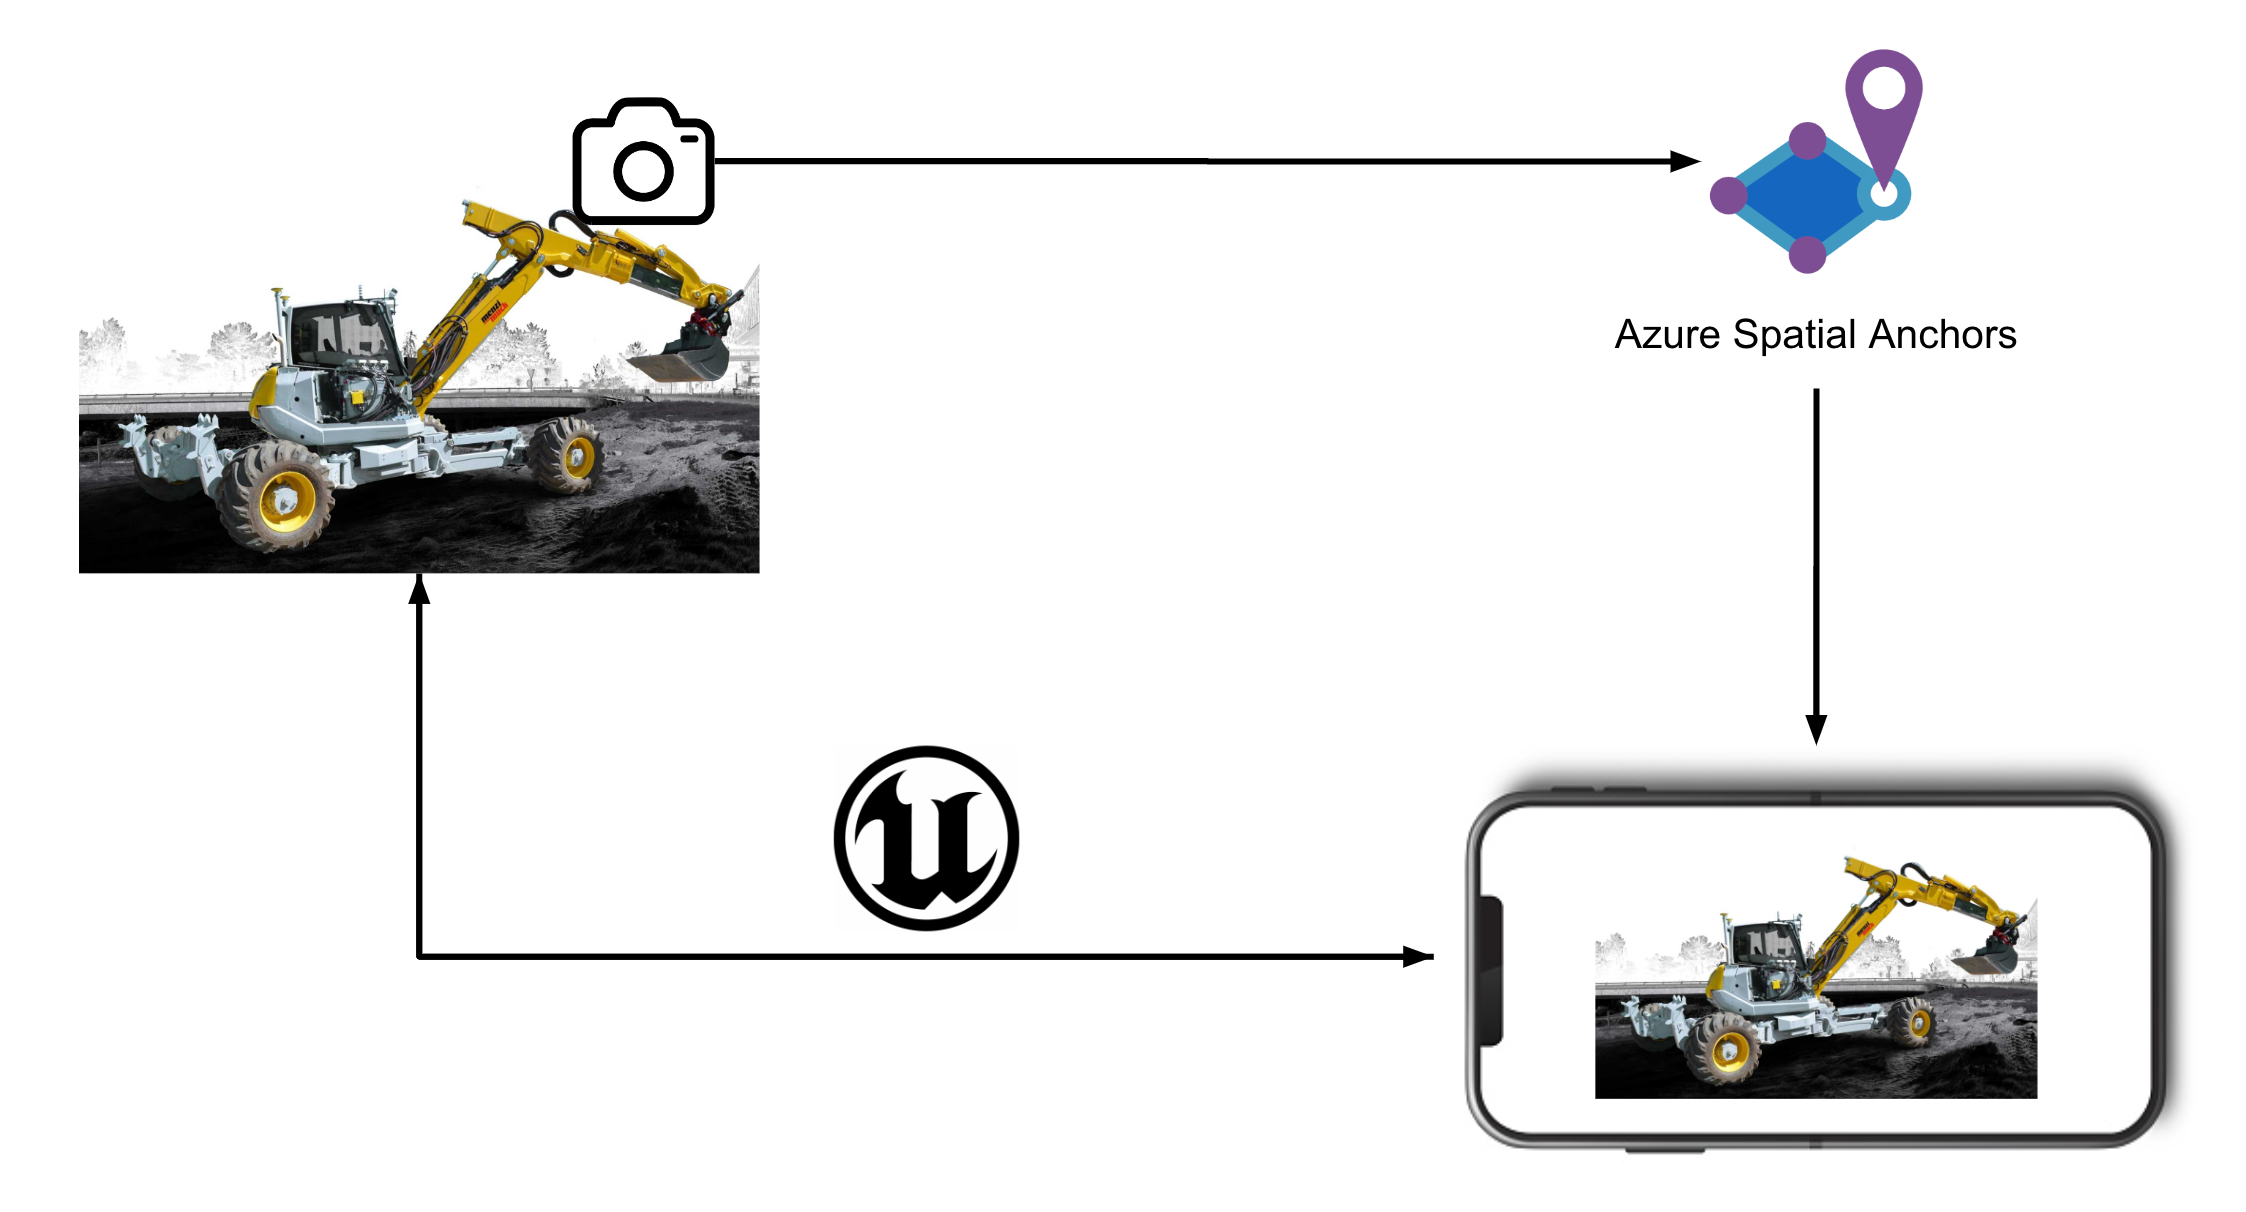
\includegraphics[scale = 0.32]{images/method/method.png}
    \caption{High level handheld remote setup}
    \label{fig:method}
\end{figure}

\begin{itemize}
    \item Data transfer between the excavator and the handheld device (left arrow connection)
    \begin{itemize}
        \item Creating an Augmented Reality Unreal Engine (UE) game on the handheld device
        \item Making use of the already existing UE interface on the excavator to store system information in game components 
        \item Using an Unreal Engine local multiplayer connection in order to transfer data between the two UE instances
    \end{itemize}
    \item Colocalization between the two frames of reference (right arrow connection) 
    \begin{itemize}
        \item Extracting a spatial anchor from the excavator's camera view using a ROS wrapper 
        \item Uploading this visual anchor in the form of an Azure Spatial Anchor to the Azure cloud
        \item Retrieving the stored spatial anchor in the handheld UE instance 
        \item Using the spatial anchor to relocate the UE world origin
    \end{itemize}
\end{itemize}





% \clearpage
% \chapter{Dataset and Complementary Image Data}\label{ch:dataset}

The LiDAR scan I worked with (Ousters OS1-128) provided 3D coordinates, returning intensity values and detected ambient lighting from the surrounding. 

This allowed for consideration of different image projections.

\section{Intensity}{
    
    This information refers to the intensity of the laser beam after being reflected from the respective surface. 
    \begin{figure}[h]
        \centering
        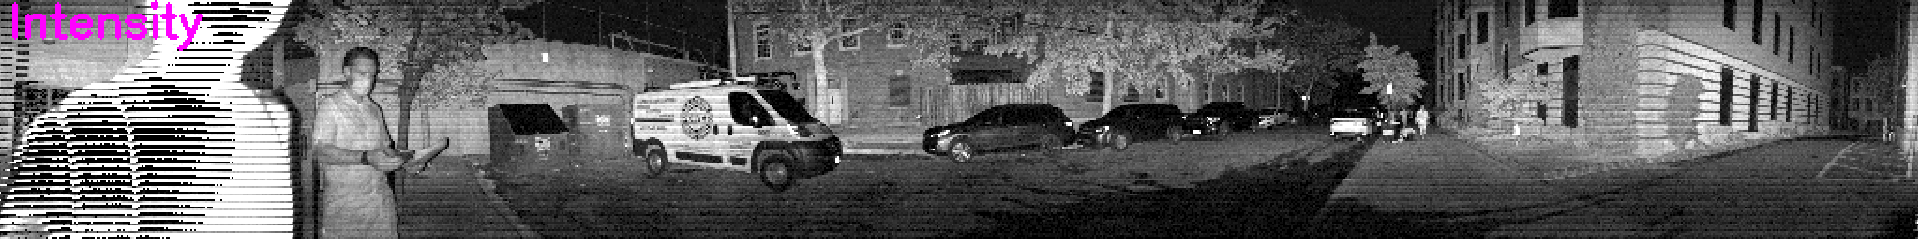
\includegraphics[scale=0.19]{images/dataset/intensity.png}
        \caption{Intensity Image Projection}
        \label{fig:intensity}
    \end{figure}
}

\section{Ambient}{

    The ambient data is the noise lighting from the surrounding. Obviously it is dependent on light however it is the closest to reality of the three data types considered.

    \begin{figure}[h]
        \centering
        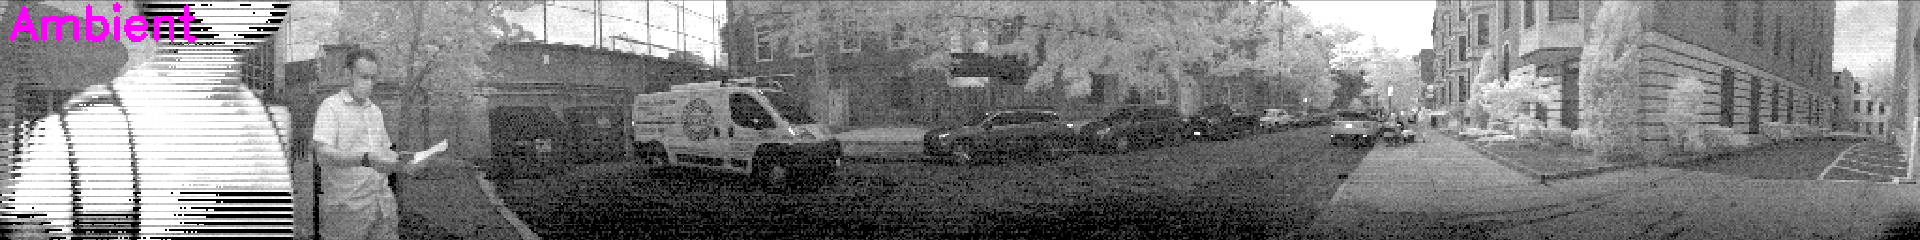
\includegraphics[scale=0.19]{images/dataset/ambient.png}
        \caption{Ambient Image Projection}
        \label{fig:ambient}
    \end{figure}
}
\clearpage

\section{Range}{
    The third data type considered was the depth. Aka each point was assigned a greyscale value depending on its normed distance towards the sensor.\\
    $\text{Range} = \sqrt{p_x^2 + p_y^2 + p_z^2} \quad$ with $p_i$ being the ith coordinate of point p.

    \begin{figure}[h]
        \centering
        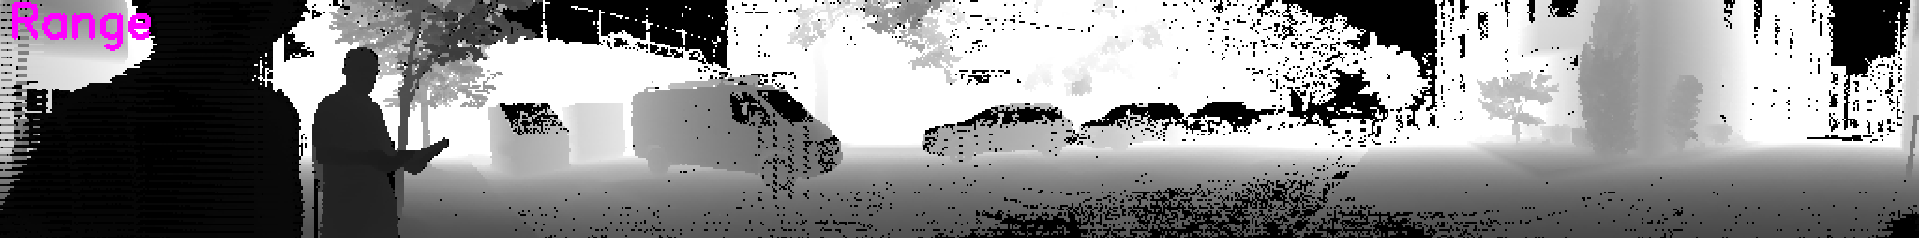
\includegraphics[scale=0.19]{images/dataset/range.png}
        \caption{Range Image Projection}
        \label{fig:range}
    \end{figure}

    
}
% \clearpage
% \chapter{Feature Extraction}\label{ch:feature_extraction}

\section{Smoothing}{
     Preceding the extraction process a smoothing\footnote{\cref{ch:smoothing}} of the images was performed to enhance the feature quality. For this dataset this was especially important because there was noise as can be seen on the intensity image projection (\cref{fig:intensity}) for example.
}


\section{Comparison Criteria}{
    On top of just extracting the features in this part I also compared different extraction methods and the aforementioned different complementary data types. The criteria for determining the quality of the feature extraction process are the amount of points detected as well as the duplicate rate of features detected repeatedly.
}

\section{Comparison of Extraction Methods}{
    For the extraction and matching procedure I used three different techniques which I wanted to compare regarding extraction, matching and of course in the end the quality of motion estimation.

    \subsection{ORB}{
        The first method considered was ORB \footnote{ORB: An efficient alternative to SIFT or SURF \citep{ORB}} (Oriented FAST and Rotated BRIEF) and as the name suggests it consists of a FAST extractor and then uses the BRIEF method with an additional rotation invariance for the description process.
        In addition to scale and rotational invariance it also provides consistency regarding significant viewpoint change.
    }

    \subsection{BRISK}{
        As a second extraction – matching based method I chose BRISK\footnote{BRISK: Binary Robust Invariant Scalable Keypoints \citep{BRISK}}. Like ORB it is based on the FAST extractor. Similar to BRIEF its descriptor consists of 128 pixel intensity comparisons which for the case of BRISK however is radially symmetric. BRISK shows slower performance than BRIEF, has however the advantage of rotational and scale invariance.
    }

    \subsection{KLT Optical Flow}{
        The last method in my comparison framework was no matching technique but instead the point tracking procedure of optical flow through KLT\footnote{Lucas Kanade Tracking \citep{KLT}}. 
    }
    \clearpage

    \subsection{Visual Comparison}{

        We start of with a visual comparison of the feature extraction on intensity data:

        \begin{figure}[ht]
            \centering
            \subfloat[ORB keypoints]{
                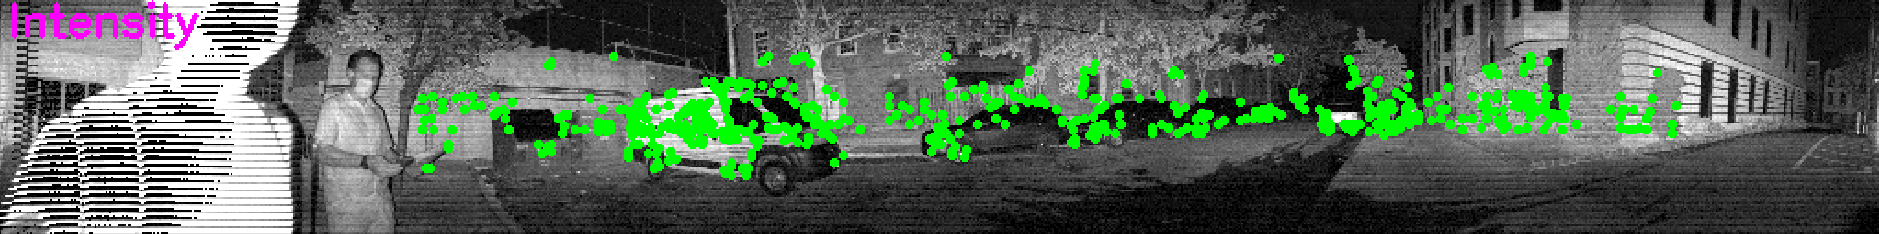
\includegraphics[scale=0.19]{images/extraction/orb.png}
                \label{fig:orb_keypoints}
            }\\
            \subfloat[BRISK keypoints]{
                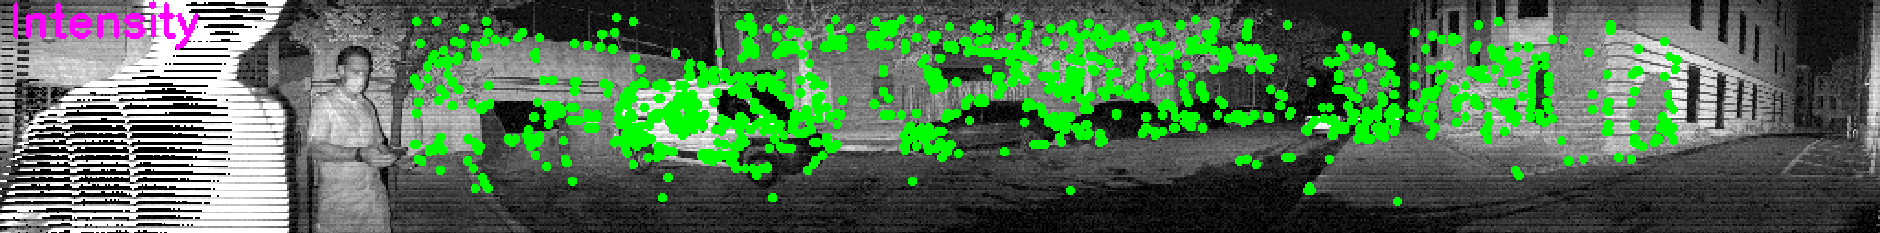
\includegraphics[scale=0.19]{images/extraction/brisk.png}
                \label{fig:brisk_keypoints}
            }\\
            \subfloat[KLT keypoints]{
                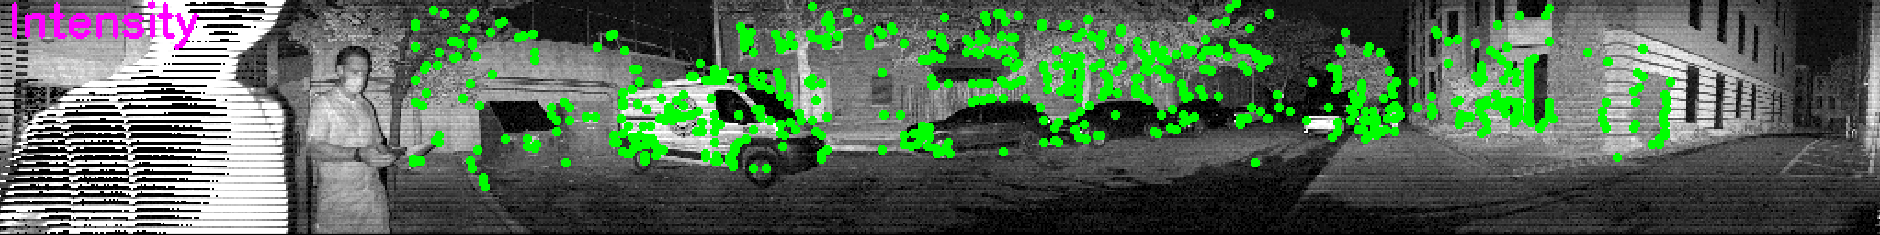
\includegraphics[scale=0.19]{images/extraction/klt.png}
                \label{fig:klt_keypoints}
            }
            \caption{Extractor Comparison}
        \end{figure}

        
        As can be seen on the images, a mask was applied to neglect features detected on the sensor holder or companion.
        From the visual comparison we can see all the methods performing reasonably well regarding the amount of features extracted. What is not visible is the rate of duplicates which was determined by applying a simple duplicate filtering and comparing the numbers.

    }

    \subsection{Statistical Comparison}{

        When considering the extraction results on intensity data over the whole duration of the 20 minute scan (12'000 scans at 10Hz) this is the comparison drawn:

        \begin{table}[!ht]
            \setlength{\extrarowheight}{5pt}
            \centering
            \large
            \begin{tabular}{cccc}
                 & \# Extracted & \# Non-Duplicates & Non-Duplicate Rate\\[12pt]
                \hline
                ORB & 529 & 521 & 98.6\\[12pt]
                \hline
                BRISK & 722 & 699 & 96.8\\[12pt]
                \hline
                KLT & 477 & 477 & 100\\[12pt]
                \hline
            \end{tabular}
            \caption{Extraction Comparison regarding Methods}
            \label{tab:extraction_methods}
        \end{table}
        
        The first result that sticks out is the 100\% non-duplicate rate for KLT which is owed to the fact that KLT has a built-in duplicate rejection mechanism. Apart from that it is worth mentioning that KLT can't be compared exactly to the other methods as it doesn't extract features each step but rather tracks them. With that in mind we see that BRISK extracts significantly more features than ORB and KLT extracts the fewest on average. Lastly overall the duplicate rates seem acceptable. Thus no preference can be voiced so far regarding the different feature methods used.
        
    }


}
\clearpage

\section{Complementary Data Comparison}{
    In the following the ORB method is used on all image types:
    \subsection{Visual Comparison - projection data types}{
    \begin{figure}[ht]
        \centering
        \subfloat[Intensity keypoints]{
            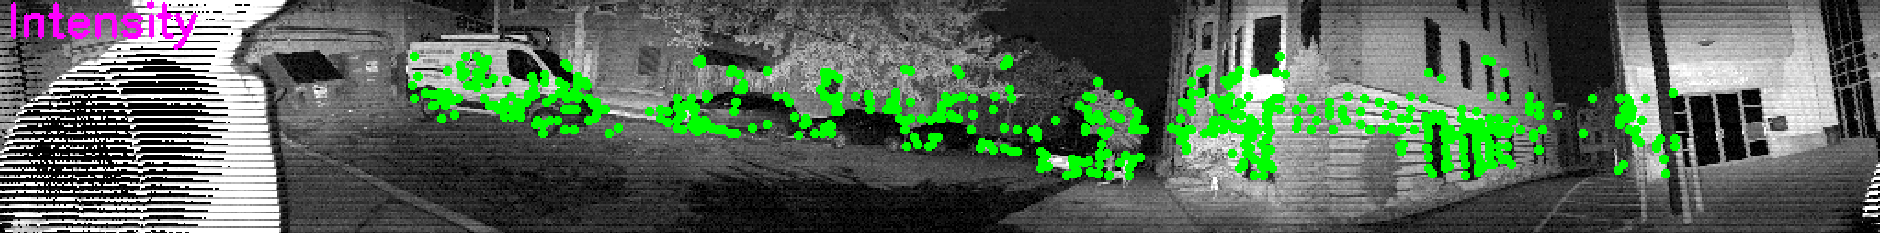
\includegraphics[scale=0.19]{images/extraction/intensity.png}
            \label{fig:intensity_keypoints}
        }\\
        \subfloat[Ambient keypoints]{
            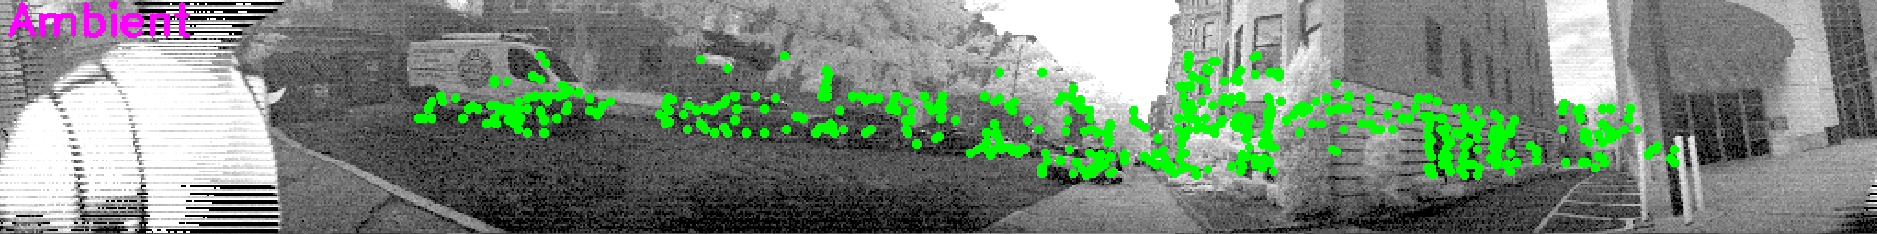
\includegraphics[scale=0.19]{images/extraction/ambient.png}
            \label{fig:ambient_keypoints}
        }\\
        \subfloat[Range keypoints]{
            
\includegraphics[scale=0.19]{images/extraction/range.png}
            \label{fig:range_keypoints}
        }
        \caption{Extraction Comparison of Complementary Data}
    \end{figure}

    Intensity and ambient both seem to perform well while range detects noticeably fewer points than the other two. Another observation is that the furthest range features result from the gradient of detected to non-reflected points in the sky. These are somewhat artificial features which might already be an indication of suboptimal performance.
    }
    \subsection{Statistical Comparison - projection data types}{

    Considering the average numbers over the whole duration:

    \begin{table}[!ht]
        \setlength{\extrarowheight}{10pt}
        \centering
        \large
        \begin{tabular}{cccc}
             & \# Extracted & \# Non-Duplicates & Non-Duplicate Rate\\[12pt]
            \hline
            Intensity & 529 & 521 & 98.6\\[12pt]
            \hline
            Ambient & 433 & 428 & 98.7\\[12pt]
            \hline
            Range & 256 & 254 & 99.25\\[12pt]
            \hline
        \end{tabular}
        \caption{Extraction Comparison regarding Methods}
        \label{tab:extraction_data}
    \end{table}

    Here the statistics repeat the story of the visual comparison. Intensity and Ambient provide similar numbers of extracted features while on the range image significantly fewer points are detected. However all data types seem viable regarding duplicate detection.

    }

}
% \clearpage
% \chapter{Feature Matching and Outlier Rejection}\label{ch:matching}

The key idea of this work revolved around building 2D matches of points of which the 3D information was known. So in essence I built 3D matches using 2D methods.
\begin{figure}[ht]
    \centering
    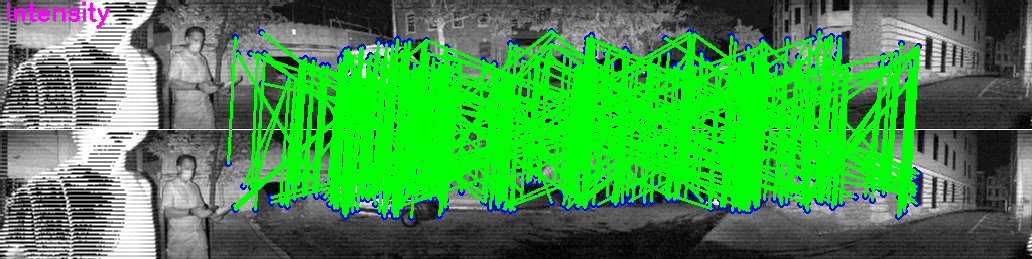
\includegraphics[scale = 0.34]{images/matching_+_outlier_rejection/orb_matches_unfiltered.png}
    \caption{Unfiltered ORB matches on intensity data}
    %label always in the end
    \label{fig:match_preview}
\end{figure}


Note that the upper half of \cref{fig:match_preview} is the current one while the lower part holds the previous stance with the detected points from the last extraction.

In order to compare the feature methods as well as the complementary data types the outlier rejection procedure has to be discussed.

\section{RANSAC Filtering}{
    The first filtering method performed was the well known non-deterministic RANSAC outlier Rejection. 
    Thanks to the projection based approach in this work a 2D – 2D RANSAC implementation could be applied.Concretely I made use of the RANSAC implementation in opencv's \textit{findHomography} method.

    \begin{figure}[ht]
        \centering
        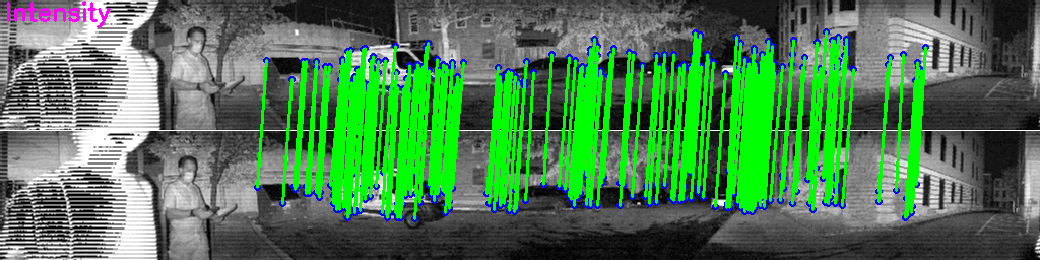
\includegraphics[scale=0.34]{images/matching_+_outlier_rejection/orb_matches_ransac_filtered.png}
        \caption{Ransac filtered}
        %label always in the end
        \label{fig:ransac_preview}
    \end{figure}
}

\section{Depth Problem}{
    The second match filtering performed accounted for depth inaccuracies for the matches considered. Just looking at the RANSAC filtered matches \cref{fig:ransac_preview} no flaw could really be detected. However as we are looking at 2D projections of 3D data we have to consider the depth as well. 

    \begin{figure}[ht]
        \centering
        \subfloat[RANSAC filtered matches]{
        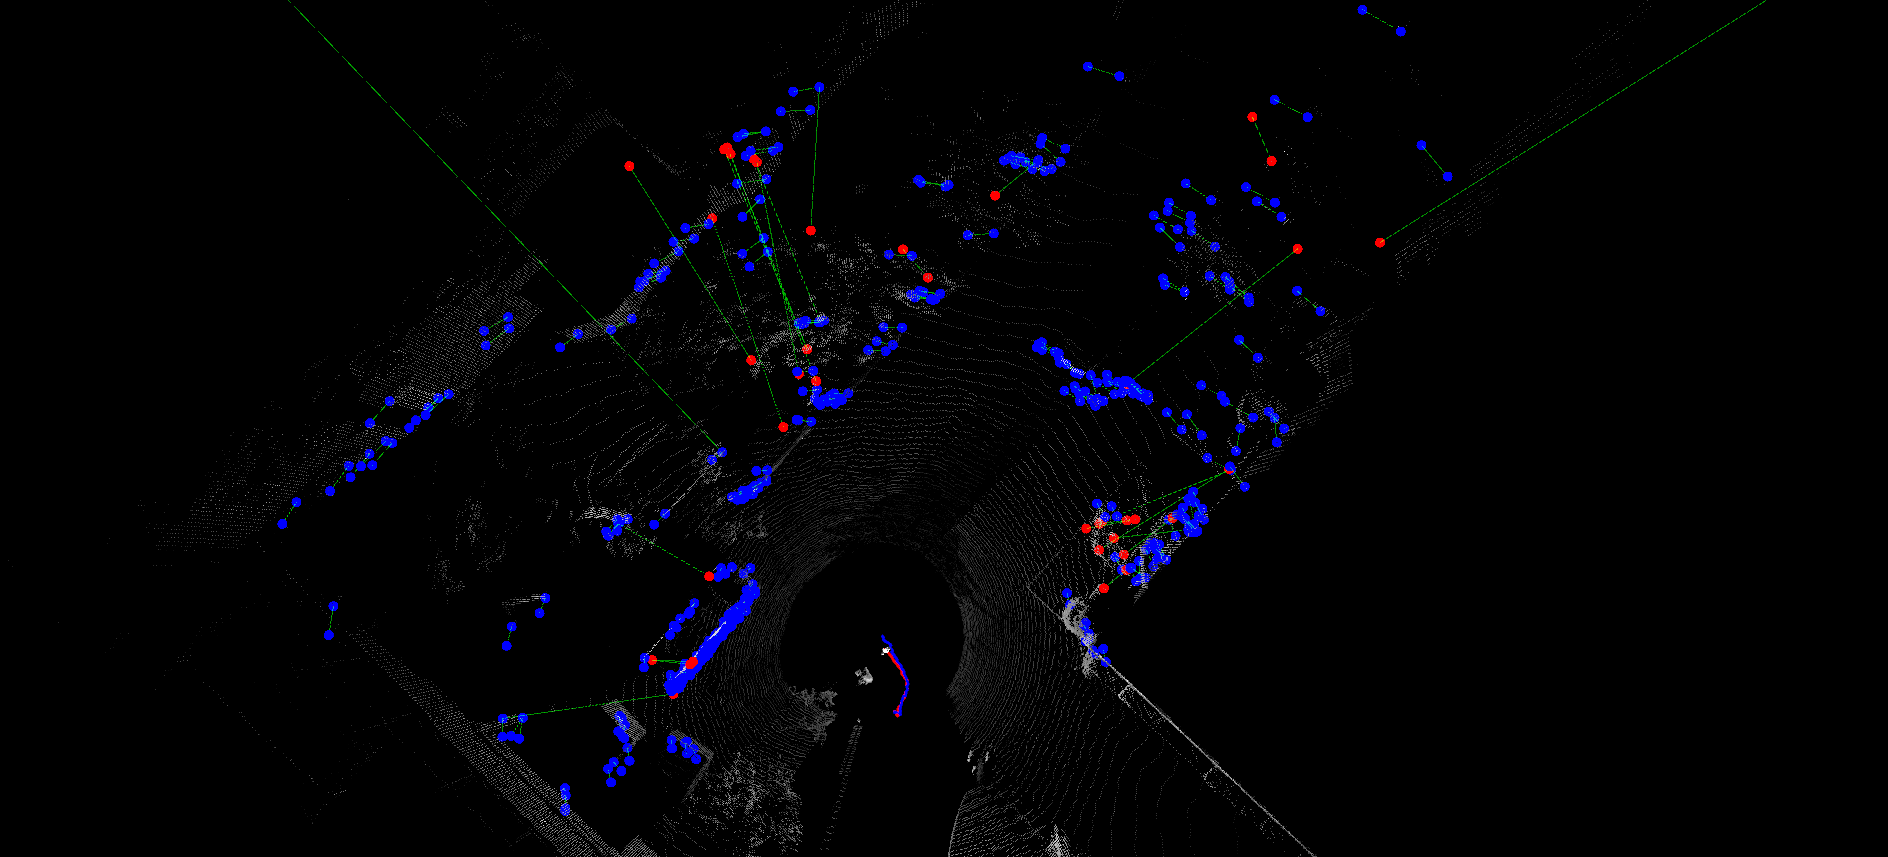
\includegraphics[scale=0.19]{images/matching_+_outlier_rejection/depth_problem_before.png}
            \label{fig:depth_before}
            }\\
        \subfloat[RANSAC + Depth filtered matches]{
        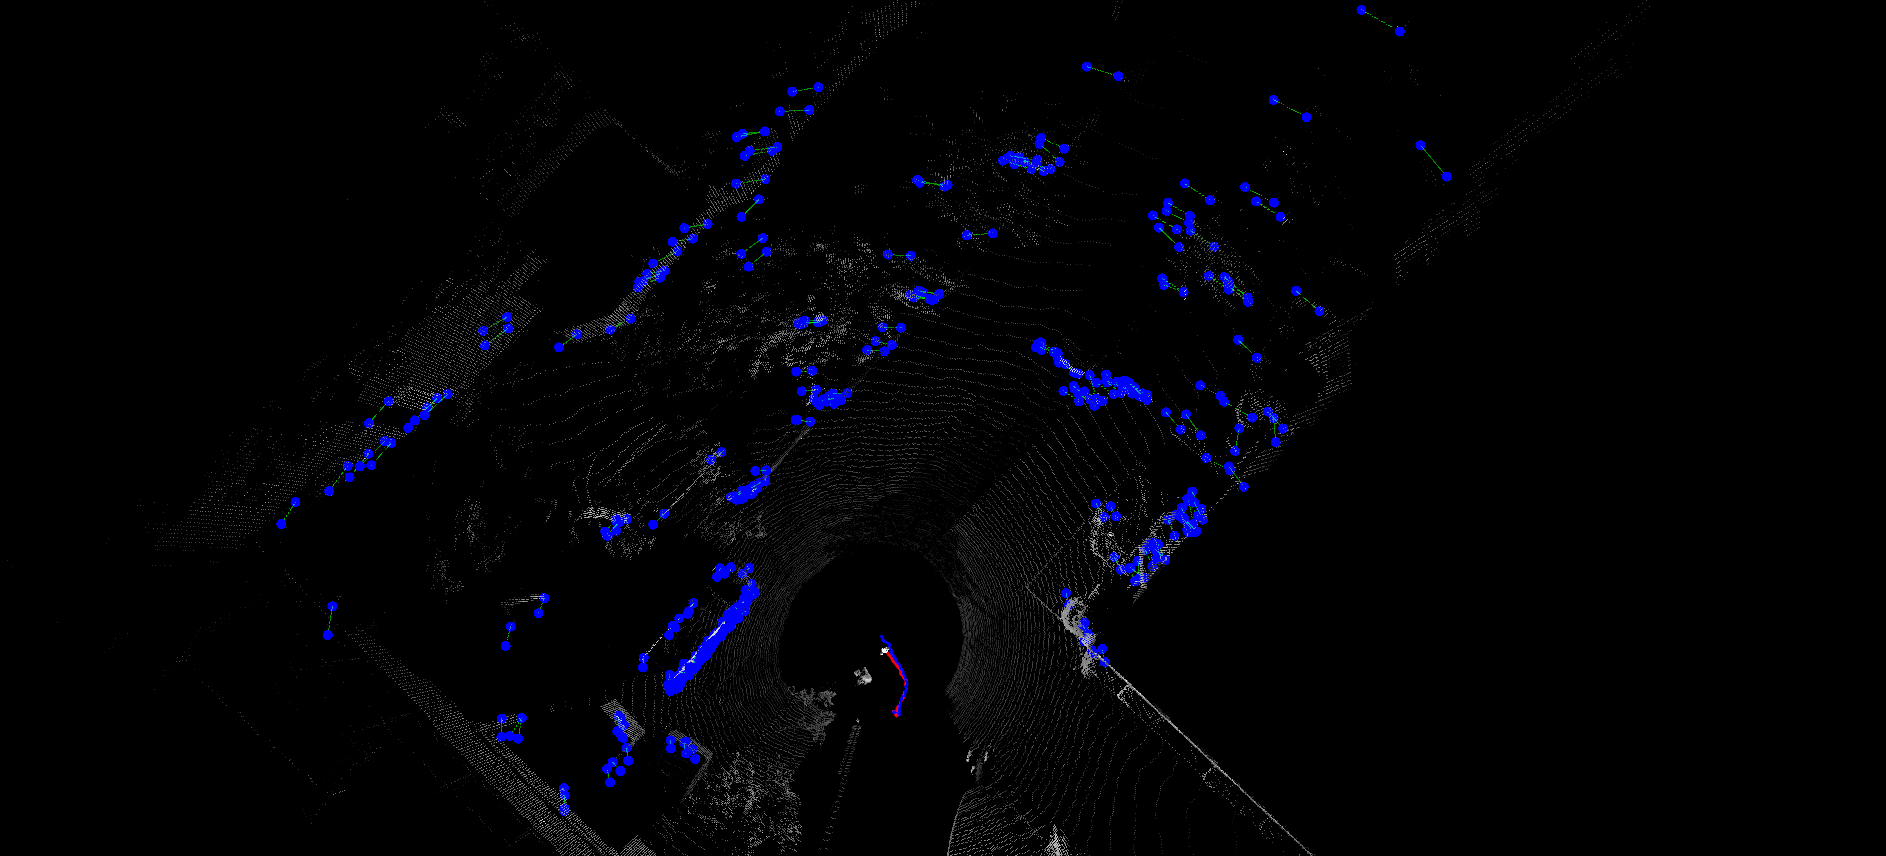
\includegraphics[scale=0.19]{images/matching_+_outlier_rejection/depth_problem_after.png}
            \label{fig:depth_after}
            }
        \caption{Depth problem visualized in Rviz}
        \label{fig:depth_problem}
    \end{figure}

    What we can see on \cref{fig:depth_problem} are correct 3D point correspondences (blue) as well as wrong matches due to depth disparity (red). Note that RANSAC doesn't filter out these red points as they comply with the 2D alignment by chance.

    To resolve this problem the following depth filtering was applied:
}

\clearpage

\section{Depth Filtering}{
    The idea was to filter out all matches with a matching distance in depth direction that surpassed a maximum threshold. To do this I considered two vectors – One from the sensor to a key point (\color{Green}OA\color{black}) and one being the matching vector (\color{orange}AB\color{black}). 

    \begin{figure}[ht]
        \centering
        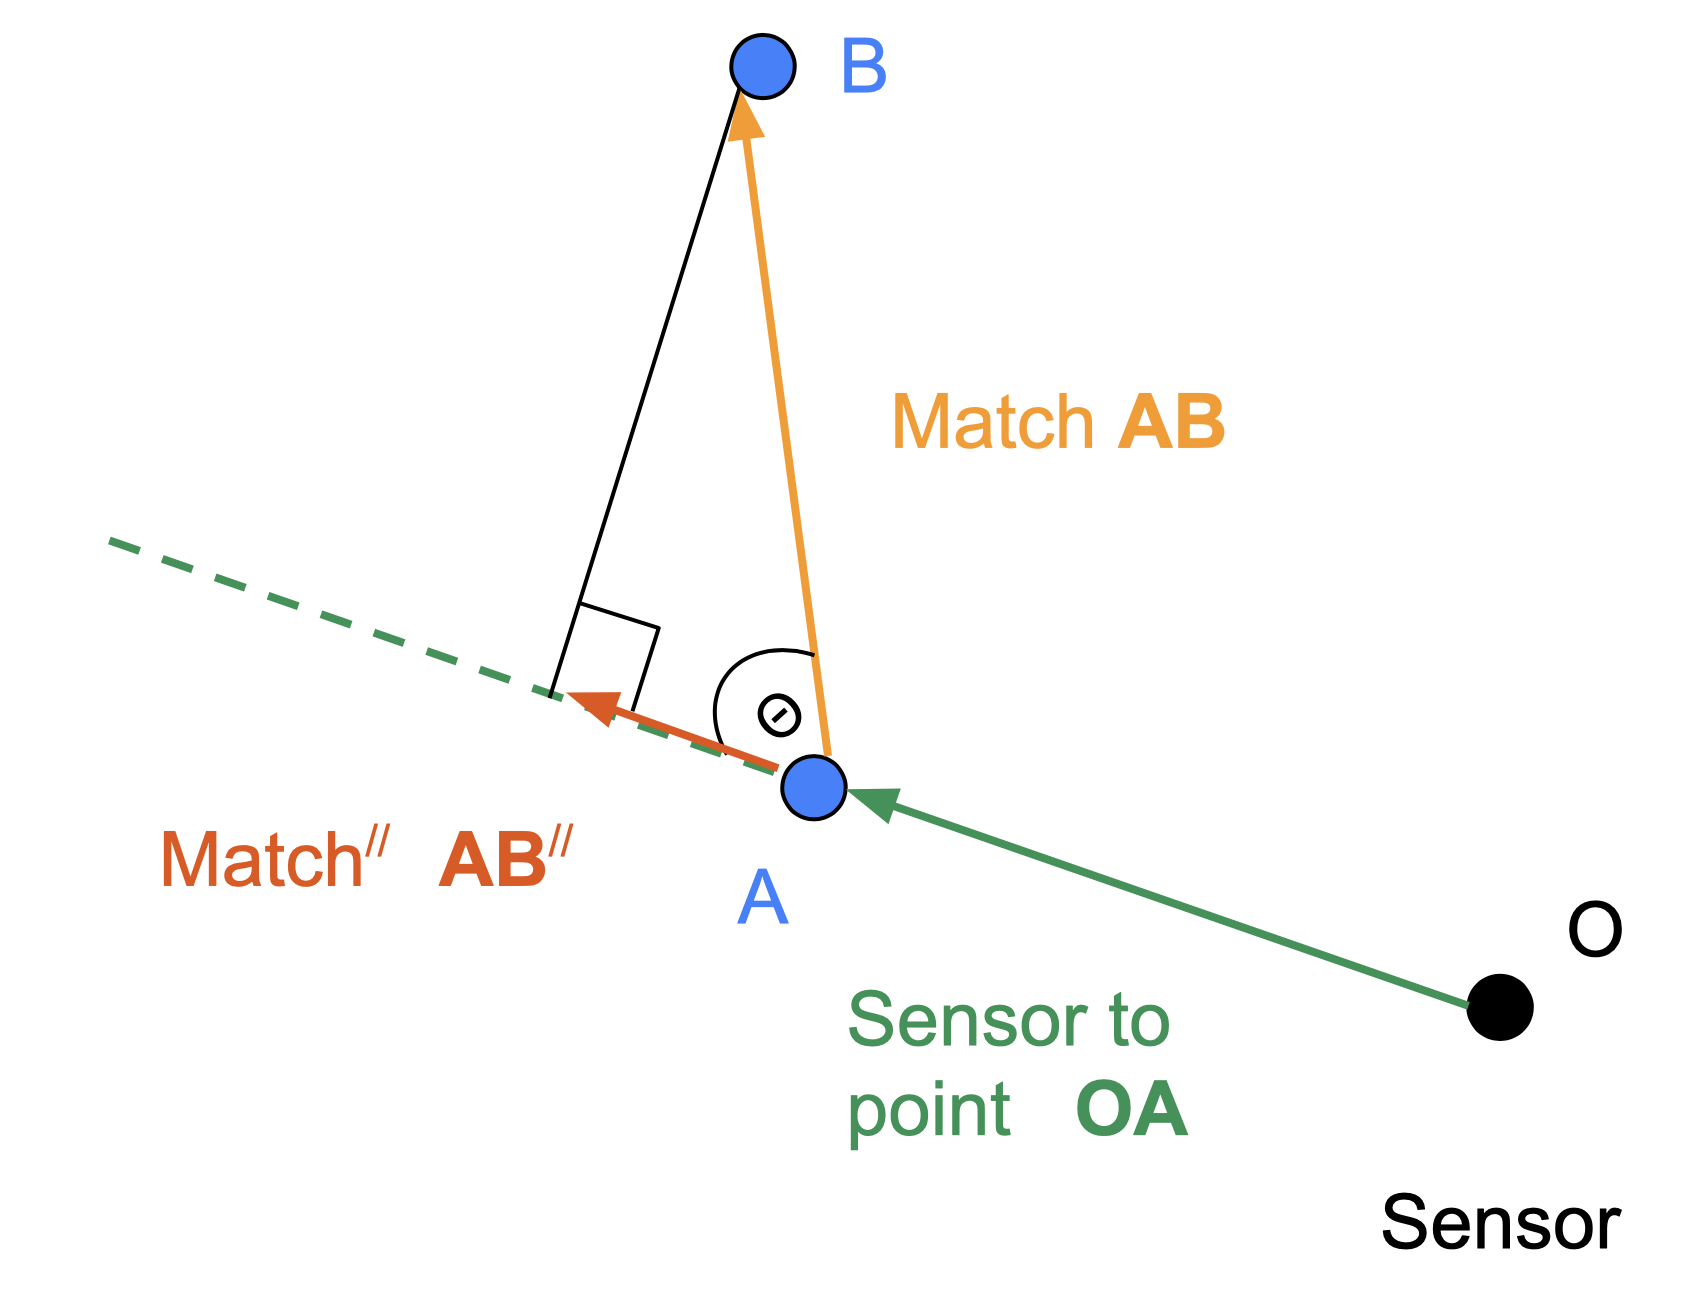
\includegraphics[scale=0.3]{images/matching_+_outlier_rejection/depth_filtering.png}
        \caption{Depth Distance}
        \label{fig:depth_distance}
    \end{figure}

    Then for the filtering I simply considered the projection of AB in depth direction
    
    \begin{center}
        \Large
        $\text{\color{BrickRed}AB\color{black}}^{||} = \frac{\left< \text{\color{Green}OA\color{black}}, \color{orange}AB\color{black}\right>}{||\text{\color{orange}AB\color{black}}||}$
    \end{center}
    and filter out values above a certain threshold. For the handheld dataset I considered at walking speed and 10Hz scanning frequency a distance of 0.3m yielded the best results.

    
}
\clearpage
\section{Feature Method Comparison}{
    After discussing the filtering procedure we can have a look at the match quality comparison. First we compare the different methods used on intensity data:

    \subsection{Visual Comparison}{

        \begin{figure}[htp]
            \centering
            \subfloat[ORB matches]{
                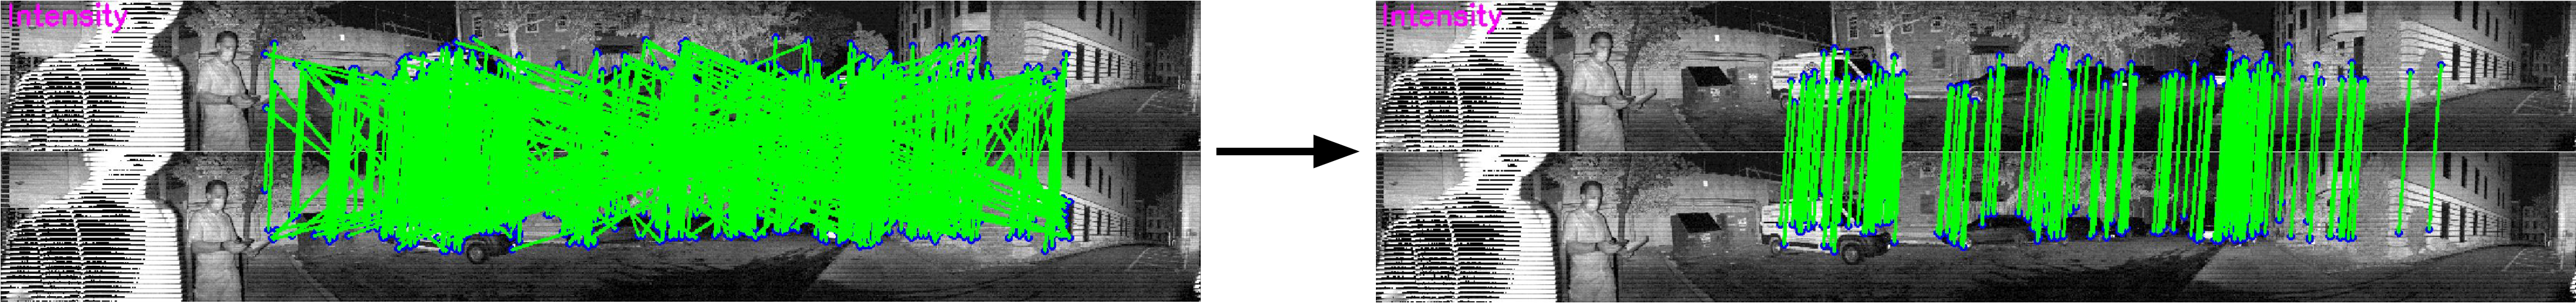
\includegraphics[scale=0.175]{images/matching_+_outlier_rejection/ORB.png}
                \label{fig:ORB_matches}
            }\\
            \subfloat[BRISK matches]{
                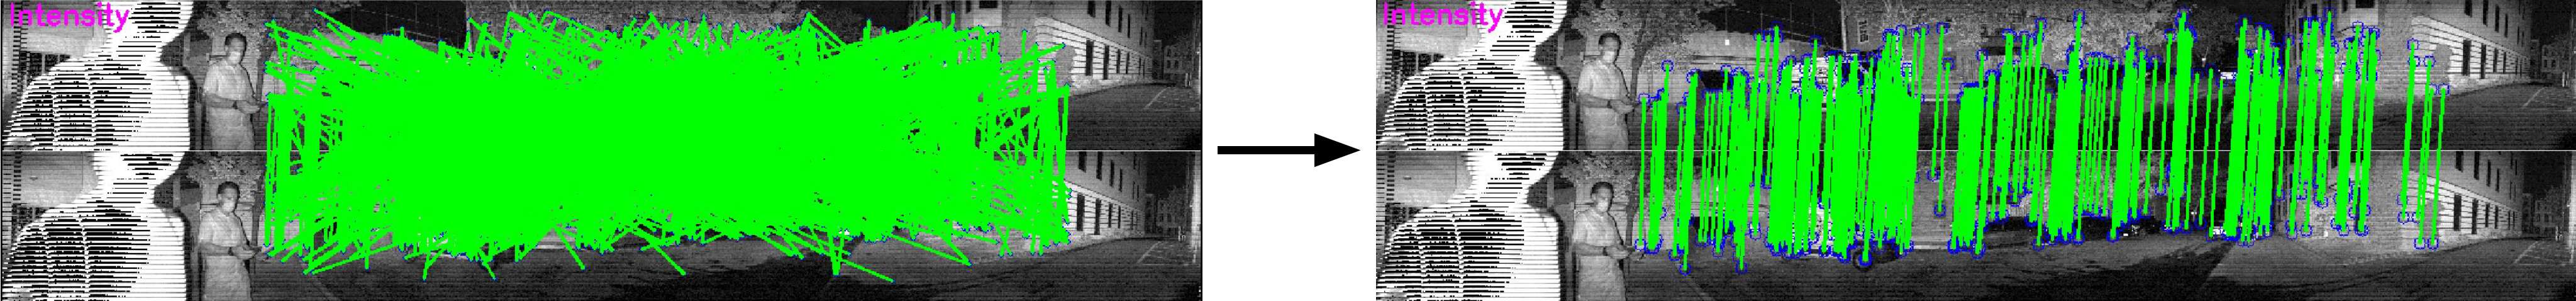
\includegraphics[scale=0.175]{images/matching_+_outlier_rejection/BRISK.png}
                    \label{fig:BRISK_matches}
            }\\
            \subfloat[KLT matches]{
                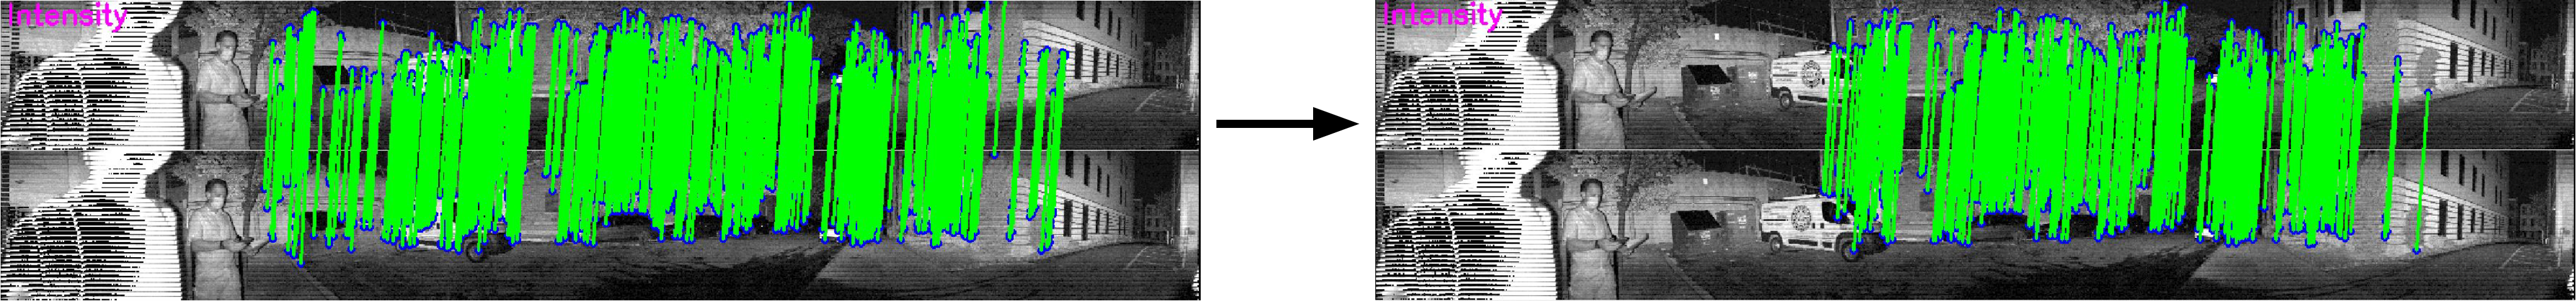
\includegraphics[scale=0.175]{images/matching_+_outlier_rejection/KLT.png}
                    \label{fig:KLT_matches}
            }\\
            \caption{Visual match comparison regarding feature methods}
            \label{fig:match_comparison_descriptors}
        \end{figure}
    
        The arrows indicate the outlier rejection procedure.
    
        As it is only one image the results to be drawn from this are fairly limited. However There seems to be a tendency of BRISK having more initial matches than the other two which complies with the previously found extraction numbers.
    }

    \subsection{Statistical Comparison}{
        As for the extraction comparison I considered the whole dataset and compared the average performance of the different feature techniques:

        \begin{table}[!ht]
            \setlength{\extrarowheight}{10pt}
            \centering
            \begin{tabular}{ccccc}
                & \# Unfiltered Matches & After RANSAC & After Depth & TP Rate [\%]\\[12pt]
                \hline
                ORB & 515 & 190 & 150 & 29.0\\[12pt]
                \hline
                BRISK & 685 & 156 & 123 & 17.9\\[12pt]
                \hline
                KLT & 186 & 151 & 136 & 72.7\\[12pt]
                \hline
            \end{tabular}
            \caption{Matching comparison between methods}
            \label{tab:matching_descriptors}
        \end{table}

        Evaluating the data we see that BRISK creates significantly more matches than ORB while losing more matches to the outlier rejection resulting in a worse TP rate. KLT has fewer correspondences (trackings of points) on average but a much higher TP rate which can be explained by the tracking nature which implicitly doesn't allow radically false  outliers.

    }


    
}

\section{Complementary Data Comparison}{
    \subsection{Visual Comparison}{
        As always the second comparison concerns the different complementary data types.

        Visual comparison using ORB on all source image types:

        \begin{figure}[htp]
            \centering
            \subfloat[Intensity matches]{
                \includegraphics[scale=0.16]{images/matching_+_outlier_rejection/Intensity.png}
                \label{fig:intensity_matches}
            }\\
            \subfloat[Ambient matches]{
                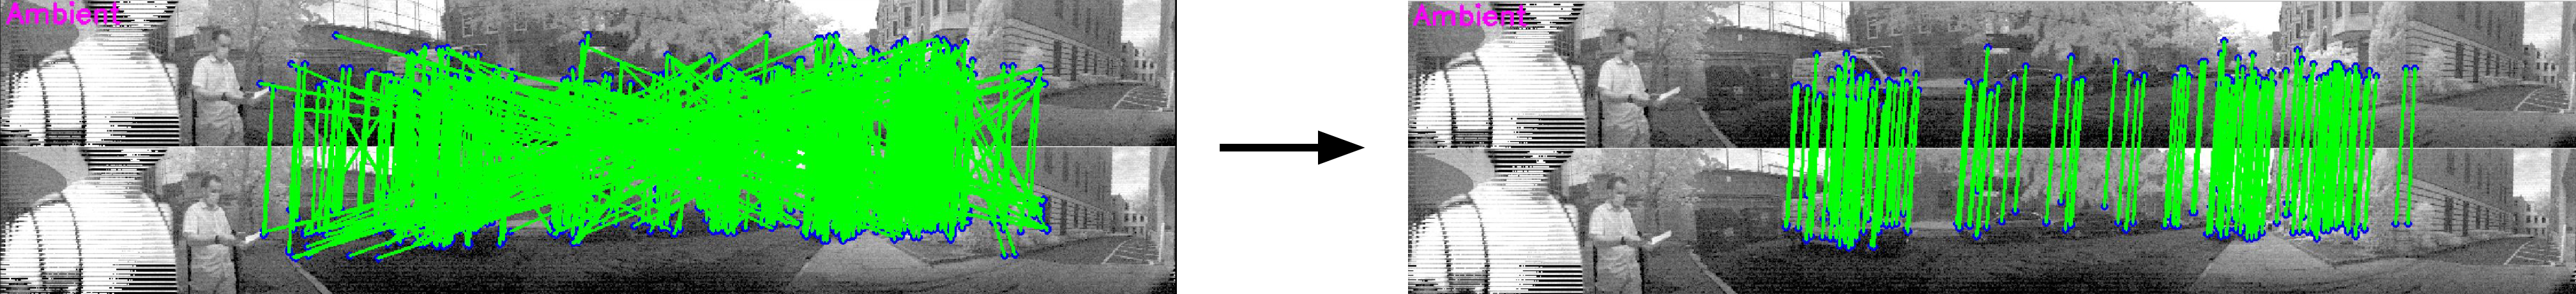
\includegraphics[scale=0.16]{images/matching_+_outlier_rejection/ambient.png}
                    \label{fig:ambient_matches}
            }\\
            \subfloat[Range matches]{
                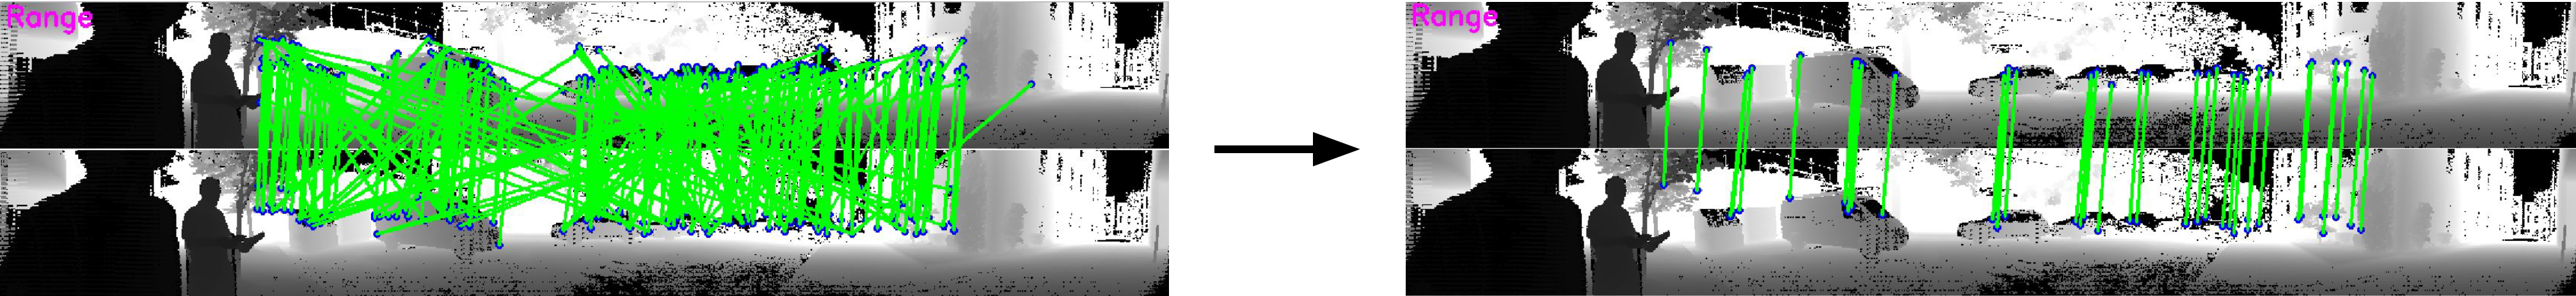
\includegraphics[scale=0.16]{images/matching_+_outlier_rejection/range.png}
                    \label{fig:range_matches}
            }\\
            \caption{Visual match comparison regarding complementary data}
            \label{fig:match_comparison_sources}
        \end{figure}

        We can again see similar performance on intensity and ambient while range has comparatively few initial matches and really few remaining filtered matches in the end.
    }
    \subsection{Statistical Comparison}{
        \begin{table}[!ht]
            \setlength{\extrarowheight}{10pt}
            \centering
            \begin{tabular}{ccccc}
                & \# Intensity Matches & After RANSAC & After Depth & TP Rate [\%]\\[12pt]
                \hline
                Intensity & 515 & 190 & 150 & 29.0\\[12pt]
                \hline
                Ambient & 421 & 164 & 123 & 29.2\\[12pt]
                \hline
                Range & 247 & 61 & 36 & 14.8\\[12pt]
                \hline
            \end{tabular}
            \caption{Matching comparison between data types}
            \label{tab:matching_data}
        \end{table}

        As can be seen ambient and intensity have really similar performance with ambient working with a little fewer matches on average. Range however performs much worse both regarding the amount of matches in general as well as the TP rate.
    }

}
% \clearpage
% \chapter{Motion Estimation}\label{ch:motion_estimation}

Instead of applying a computationally expensive iterative procedure like ICP\footnote{Iterative Closest Point \citep{Pomerleau}} I could make use of my previously found correspondences and apply the closed form solution\citep{closed_form} to the alignment problem.

So each iteration a rotation matrix \textbf{R} and a translation vector \textbf{t} are estimated.

\section{Pose update}{
    In order to track the estimated pose of the sensor a current pose is considered in homogeneous coordinates and is updated using each iterations respective rotational and translational change.

    \begin{center}
        $\text{New Pose} = 
        \underbrace{\begin{bmatrix}
            R_{11o} & R_{12o} & R_{13o} & t_1o\\
            R_{21o} & R_{22o} & R_{23o} & t_2o\\
            R_{31o} & R_{32o} & R_{33o} & t_3o\\
            0&0&0&1
        \end{bmatrix}}_{\text{Old Pose}} * 
        \underbrace{\begin{bmatrix}
            R_{11i} & R_{12i} & R_{13i} & t_1i\\
            R_{21i} & R_{22i} & R_{23i} & t_2i\\
            R_{31i} & R_{32i} & R_{33i} & t_3i\\
            0&0&0&1
        \end{bmatrix}}_{\text{Pose Update}}
        $
    \end{center}

    This pose represents the transformation from the static world frame to the dynamic sensor frame and determines the quality of this methods motion estimation procedure.
    
    For the evaluation of my method and the comparison of the individual building blocks used in my method I considered the transformation as such, the path drawn when following the pose in the world frame as well as the mapping quality when considering multiple subsequent point clouds. 
}







% \clearpage
% % \chapter{Results}\label{sec:results}

% \section{Ground Truth}{
    
%     As there wasn't a GT for my dataset I considered the very accurate and map based Lio-Sam\footnote{LIO-SAM: Tightly-coupled Lidar Inertial Odometry via Smoothing and Mapping \citep{liosam2020shan}} estimation as the GT for this work. 
    
%     I also considered LOAM\footnote{LiDAR Odometry And Mapping \citep{LOAM}} for another comparison and very importantly as a third and most meaningful alternative I chose the LOAM method without the map procedure as well. This is because my approach is scan based and does not build a map which of course enhances accuracy significantly. So comparing to a scan based method is the only fair comparison.


%     }

% \section{Stepwise Results}{

%     \subsection{Comparison of Separated Components}{
%     \begin{figure}[ht]
%         \centering
%         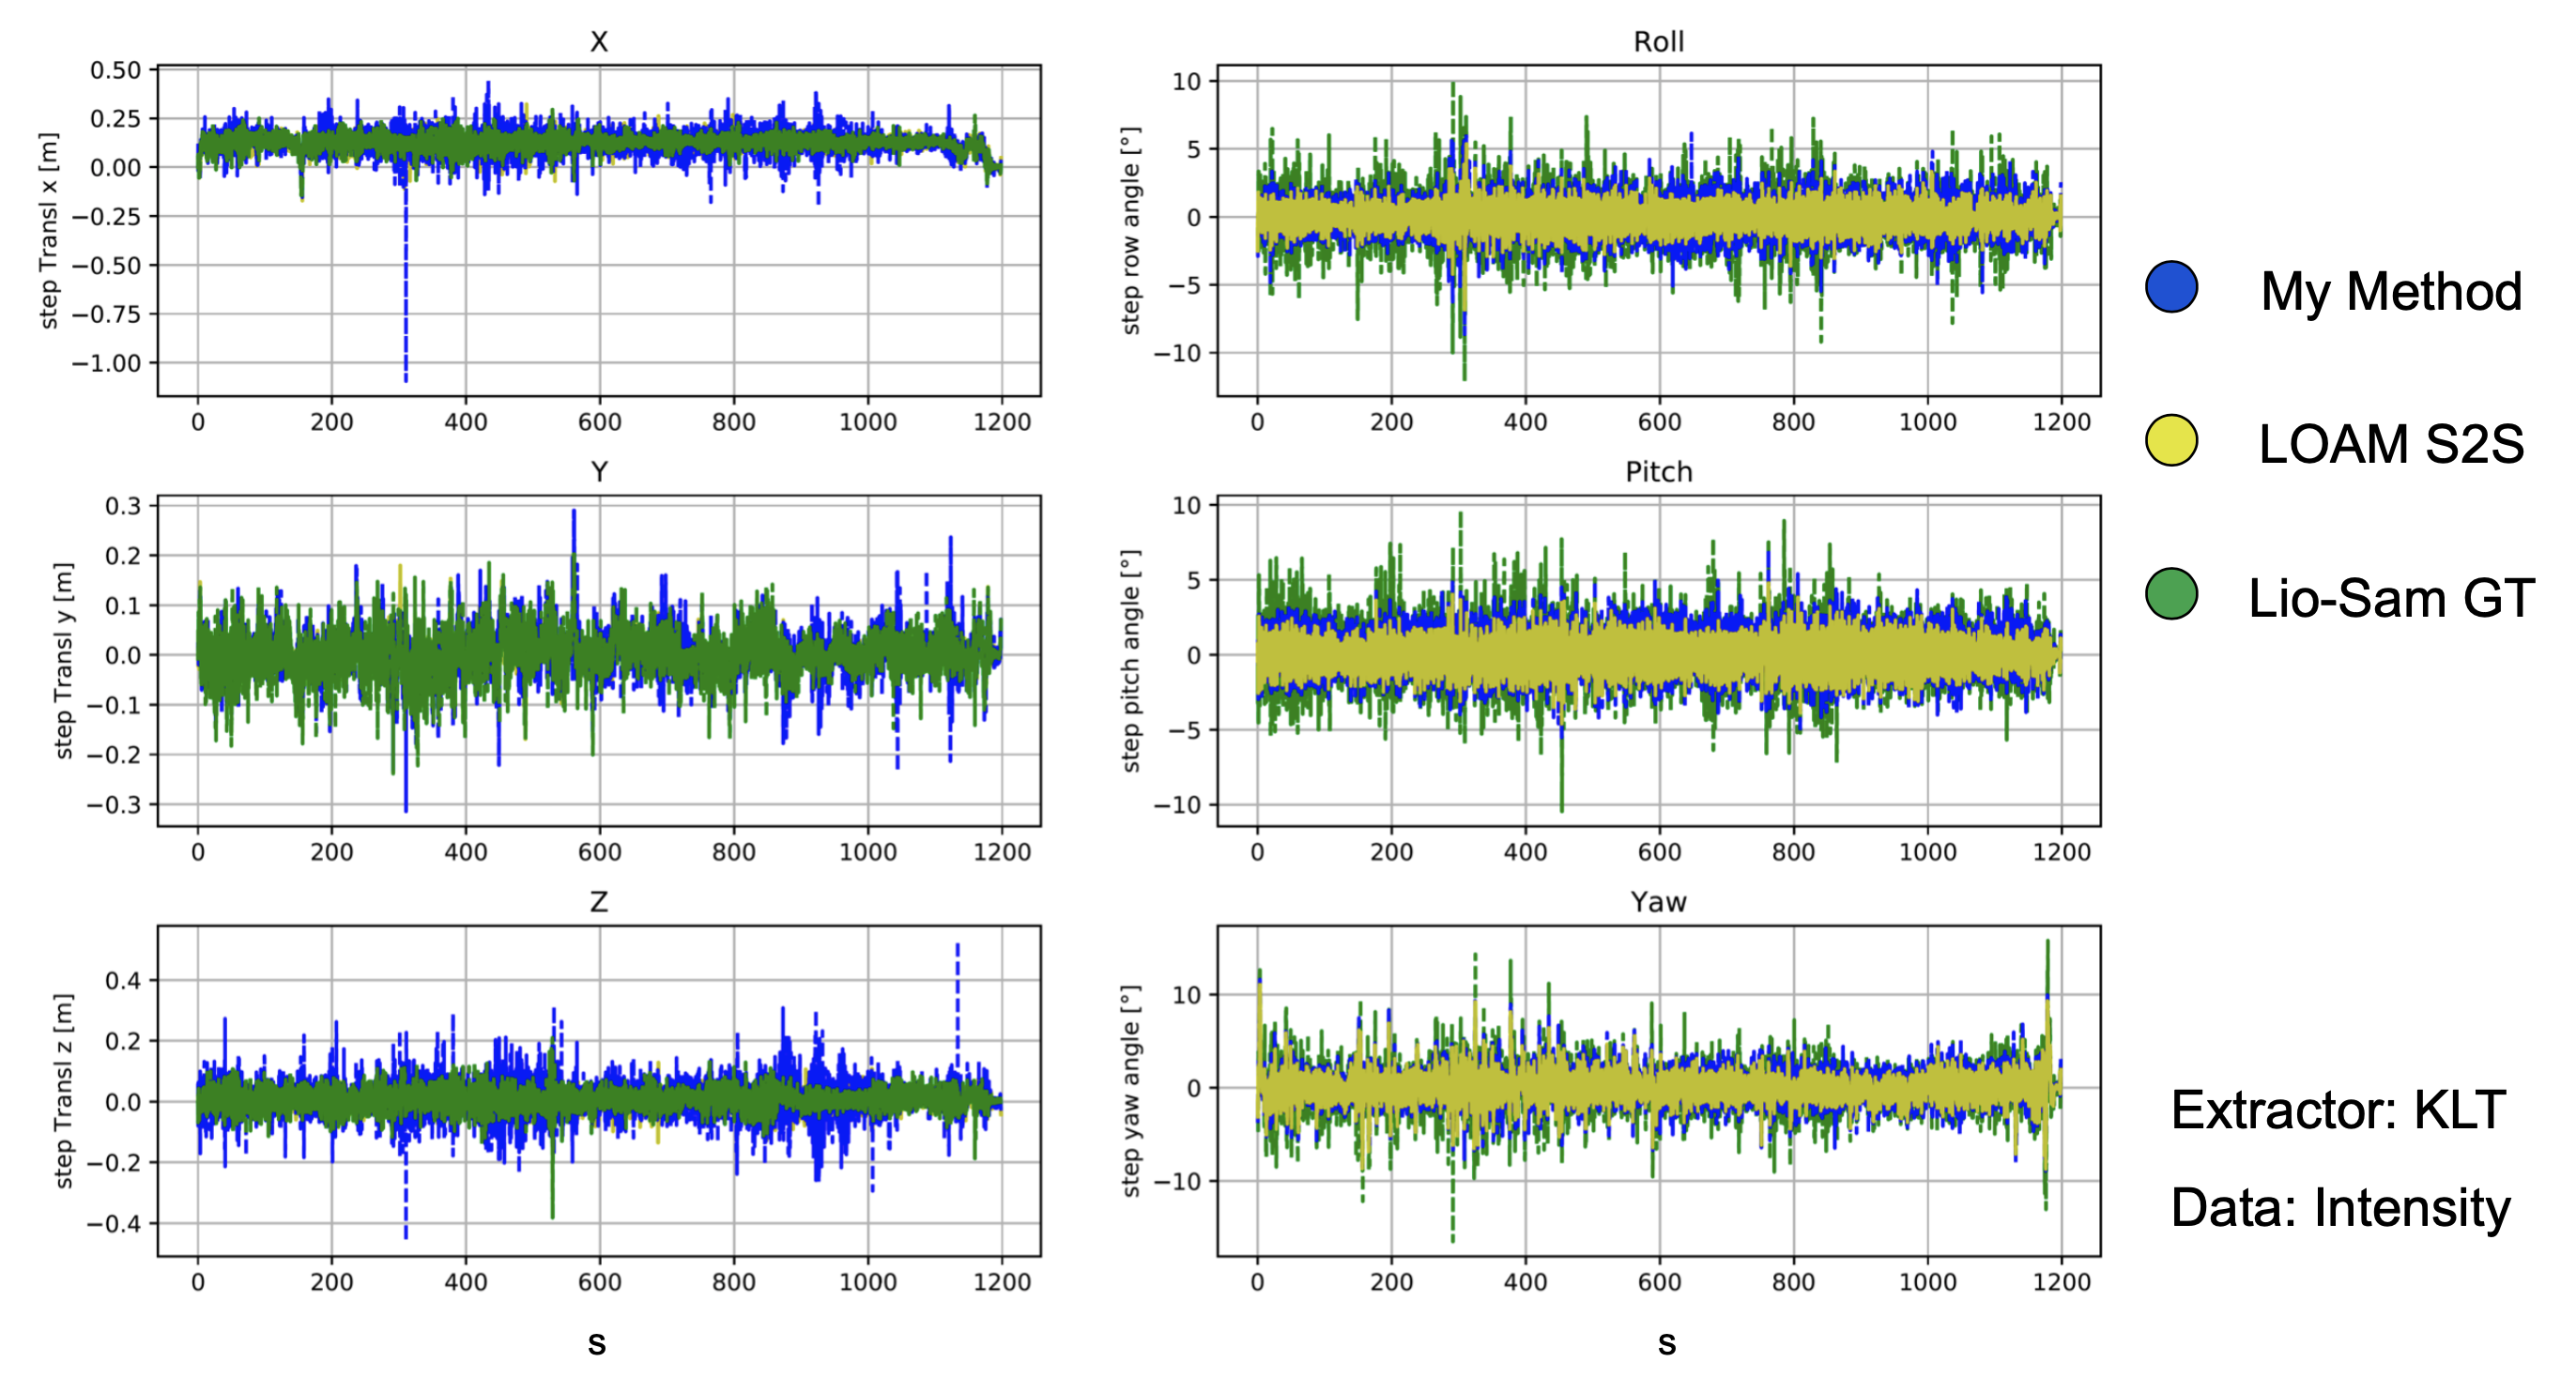
\includegraphics[scale = 0.26]{images/results/steps_klt.png}
%         \caption{Step comparison}
%         \label{fig:step_comparison_klt}
%     \end{figure}

%     In \cref{fig:step_comparison_klt} we can see the step comparison of the three directions as well as the rotation angles. 
    
%     We can also consider the errors at each iteration depicted in the following \cref{fig:step_error_comparison_klt}
%     \begin{figure}[ht]
%         \centering
%         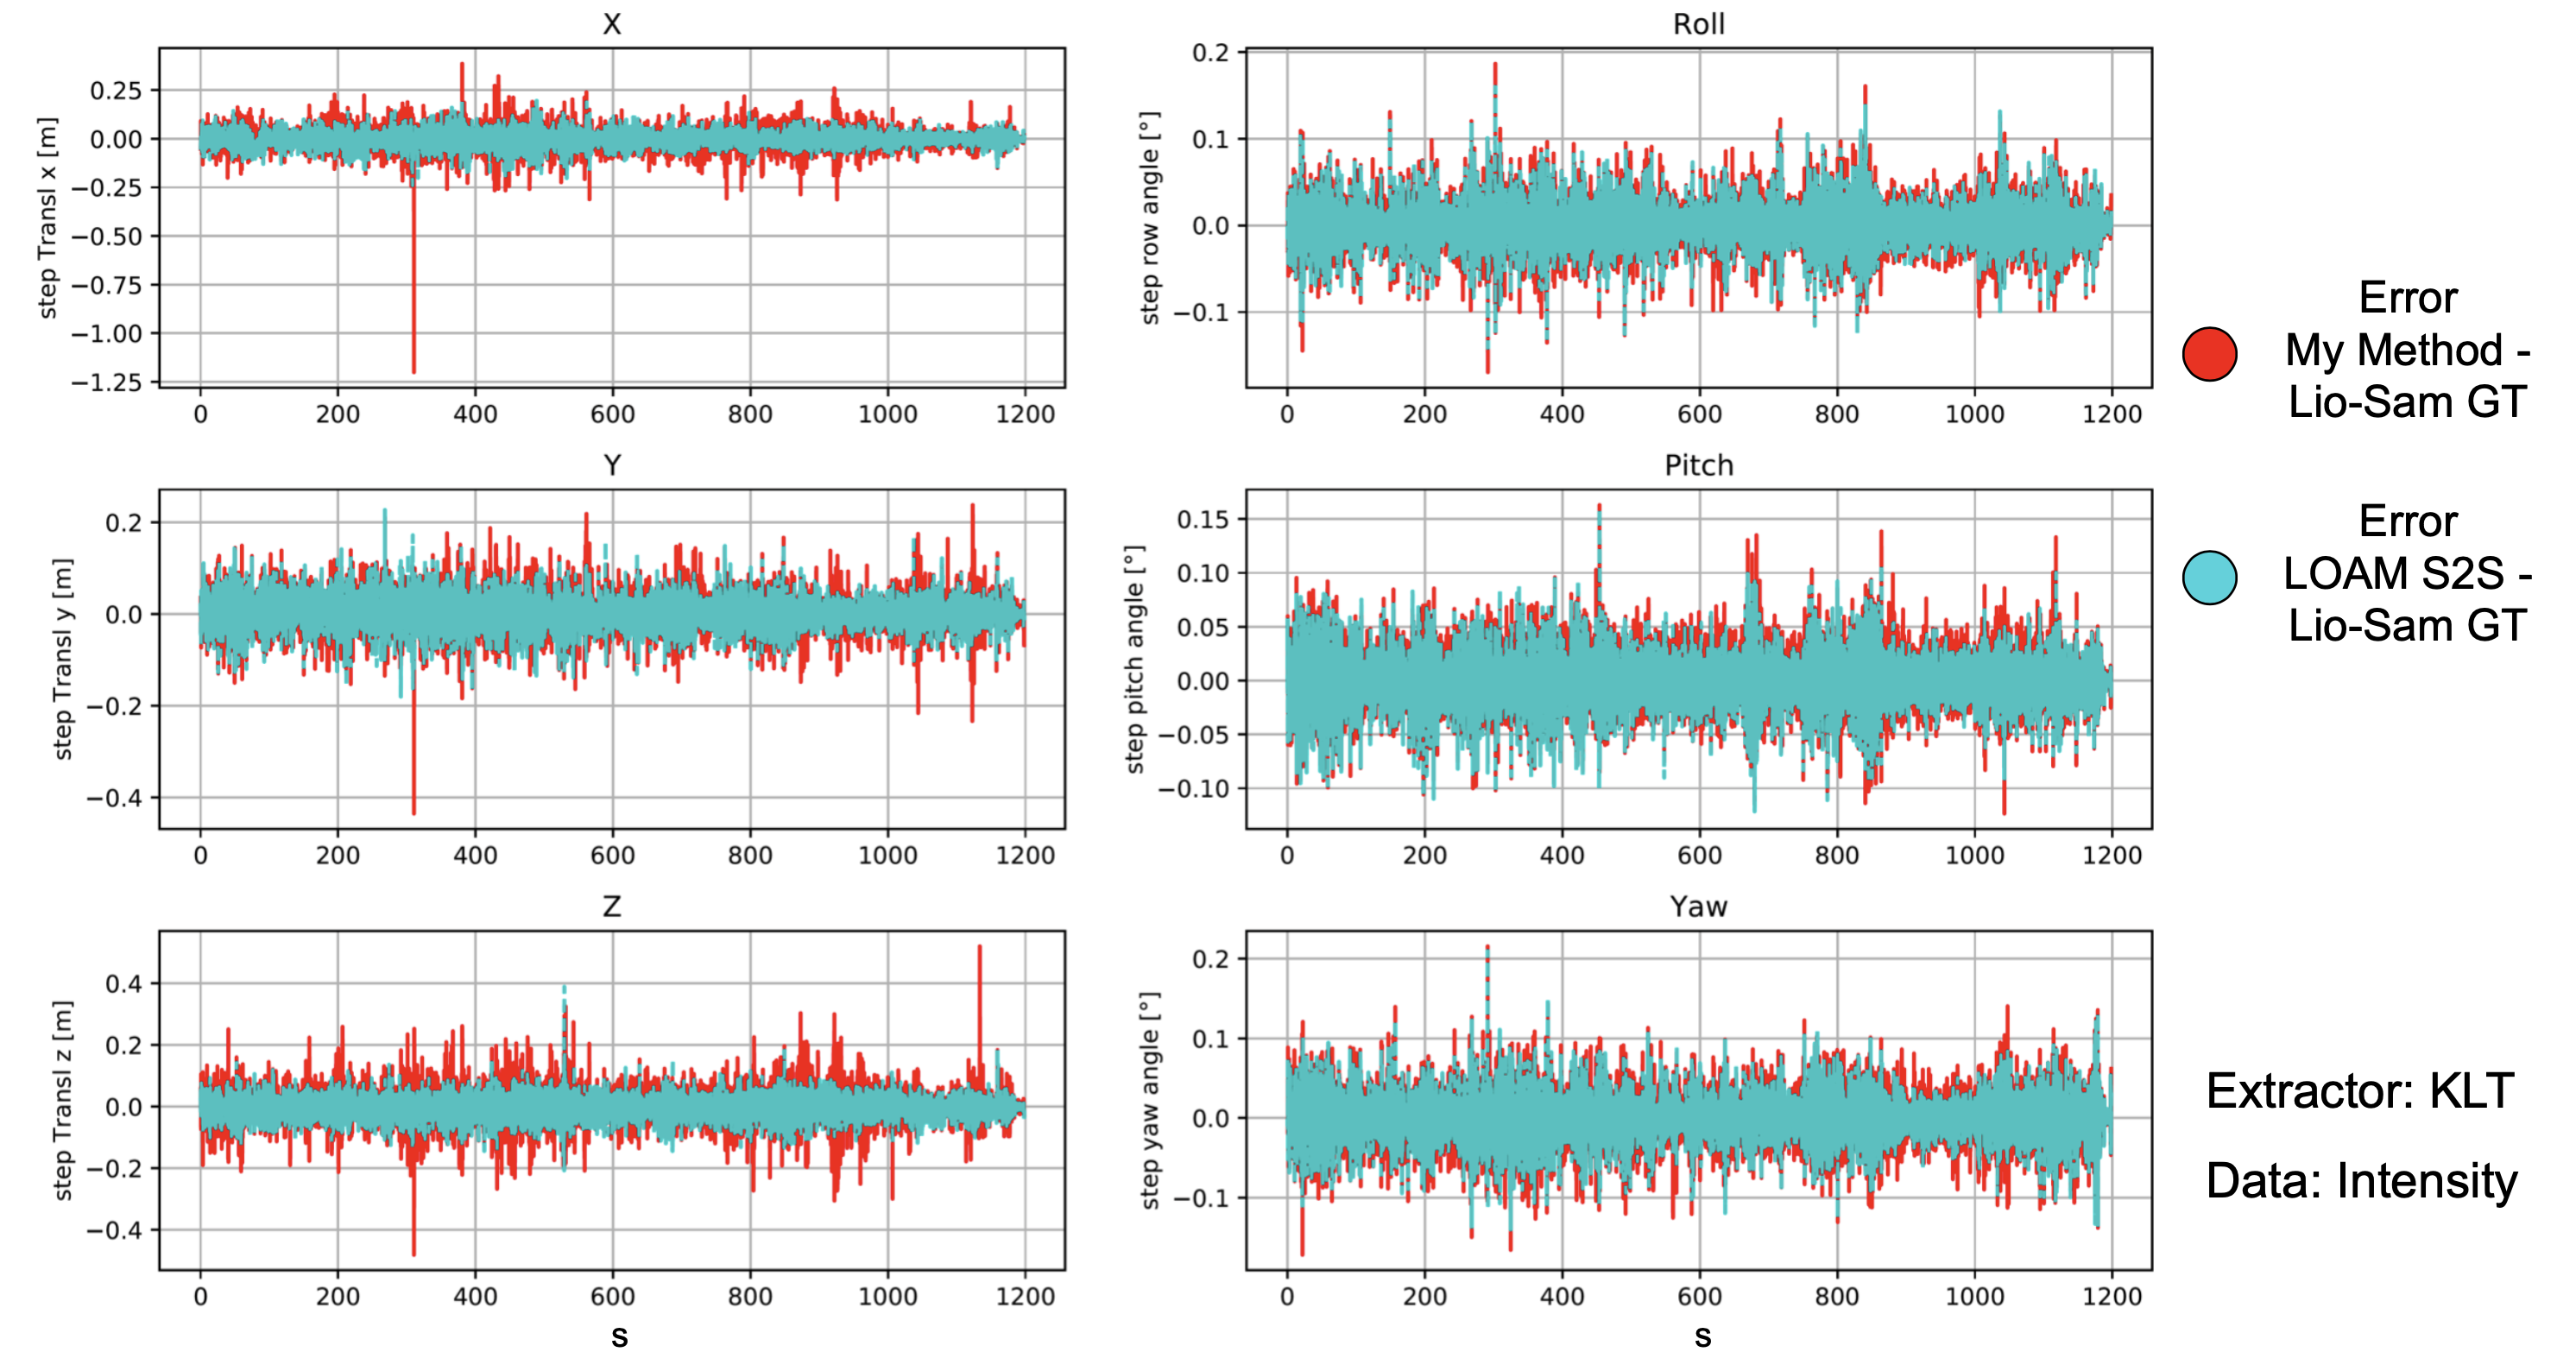
\includegraphics[scale = 0.285]{images/results/step_error_klt.png}
%         \caption{Step Error comparison}
%         \label{fig:step_error_comparison_klt}
%     \end{figure}



%     As we can see in the figures \cref{fig:step_comparison_klt} and \cref{fig:step_error_comparison_klt} there are outliers in the method. However both the step error of this papers method as well as the iterative error of the scan based LOAM method yield values in the same range.

%     }

%     \subsection{Average Step Performance Comparison}{
%     Mean iterative error and standard deviation thereof regarding GT over the whole dataset:

%         \vspace{0.5cm}
        
%         \large
%         \begin{tabular}{p{3cm} p{4.5cm} p{3.5cm} }
%             \textbf{Errors} & \textbf{My Method} & \textbf{LOAM S2S}
%         \end{tabular}

%         \begin{table}[!ht]
%             \setlength{\extrarowheight}{5pt}
%             \centering
%             \large
%             \begin{tabular}{p{2cm} p{2cm} p{2cm} p{2cm} p{2cm} }
%                 \hline
%                  & Mean & STD & Mean & STD\\[12pt]
%                 \hline
%                 X[m] & -0.004 & 0.056 & \text{\color{Green}{-0.002}} & \text{\color{Cyan}{0.035}}\\[3pt]
%                 \hline
%                 Y[m] & \text{\color{Green}{0}} & 0.040 & 0.005 & \text{\color{Cyan}{0.028}}\\[3pt]
%                 \hline
%                 Z[m] & \text{\color{Green}{-0.001}} & 0.058 & -0.004 & \text{\color{Cyan}{0.032}}\\[3pt]
%                 \hline
%                 Roll[°] & \text{\color{Green}{0}} & 0.024 & \text{\color{Green}{0}} & \text{\color{Cyan}{0.021}}\\[3pt]
%                 \hline
%                 Pitch[°] & \text{\color{Green}{0}} & 0.024 & -0.001 & \text{\color{Cyan}{0.020}}\\[3pt]
%                 \hline
%                 Yaw[°] & \text{\color{Green}{0}} & 0.024 & \text{\color{Green}{0}} & \text{\color{Cyan}{0.023}}\\[3pt]
%             \end{tabular}
%             \caption{Average Step Error Comparison}
%             \label{tab:step_errors_klt}
%         \end{table}

%         The data displayed in \cref{tab:step_errors_klt} was achieved using the KLT method on intensity data. Green values are the best achieved mean while light blue indicates the best standard deviation.   

%         When evaluating the numbers we see for my method smaller mean errors on average while LOAM scan 2 scan has smaller deviations from the slightly larger mean error.

        
%     }

% \section{Global Results}{
%     \subsection{Comparison of Separated Components}{

%     Comparing the individual pose components:

%         \begin{figure}[ht]
%             \centering
%             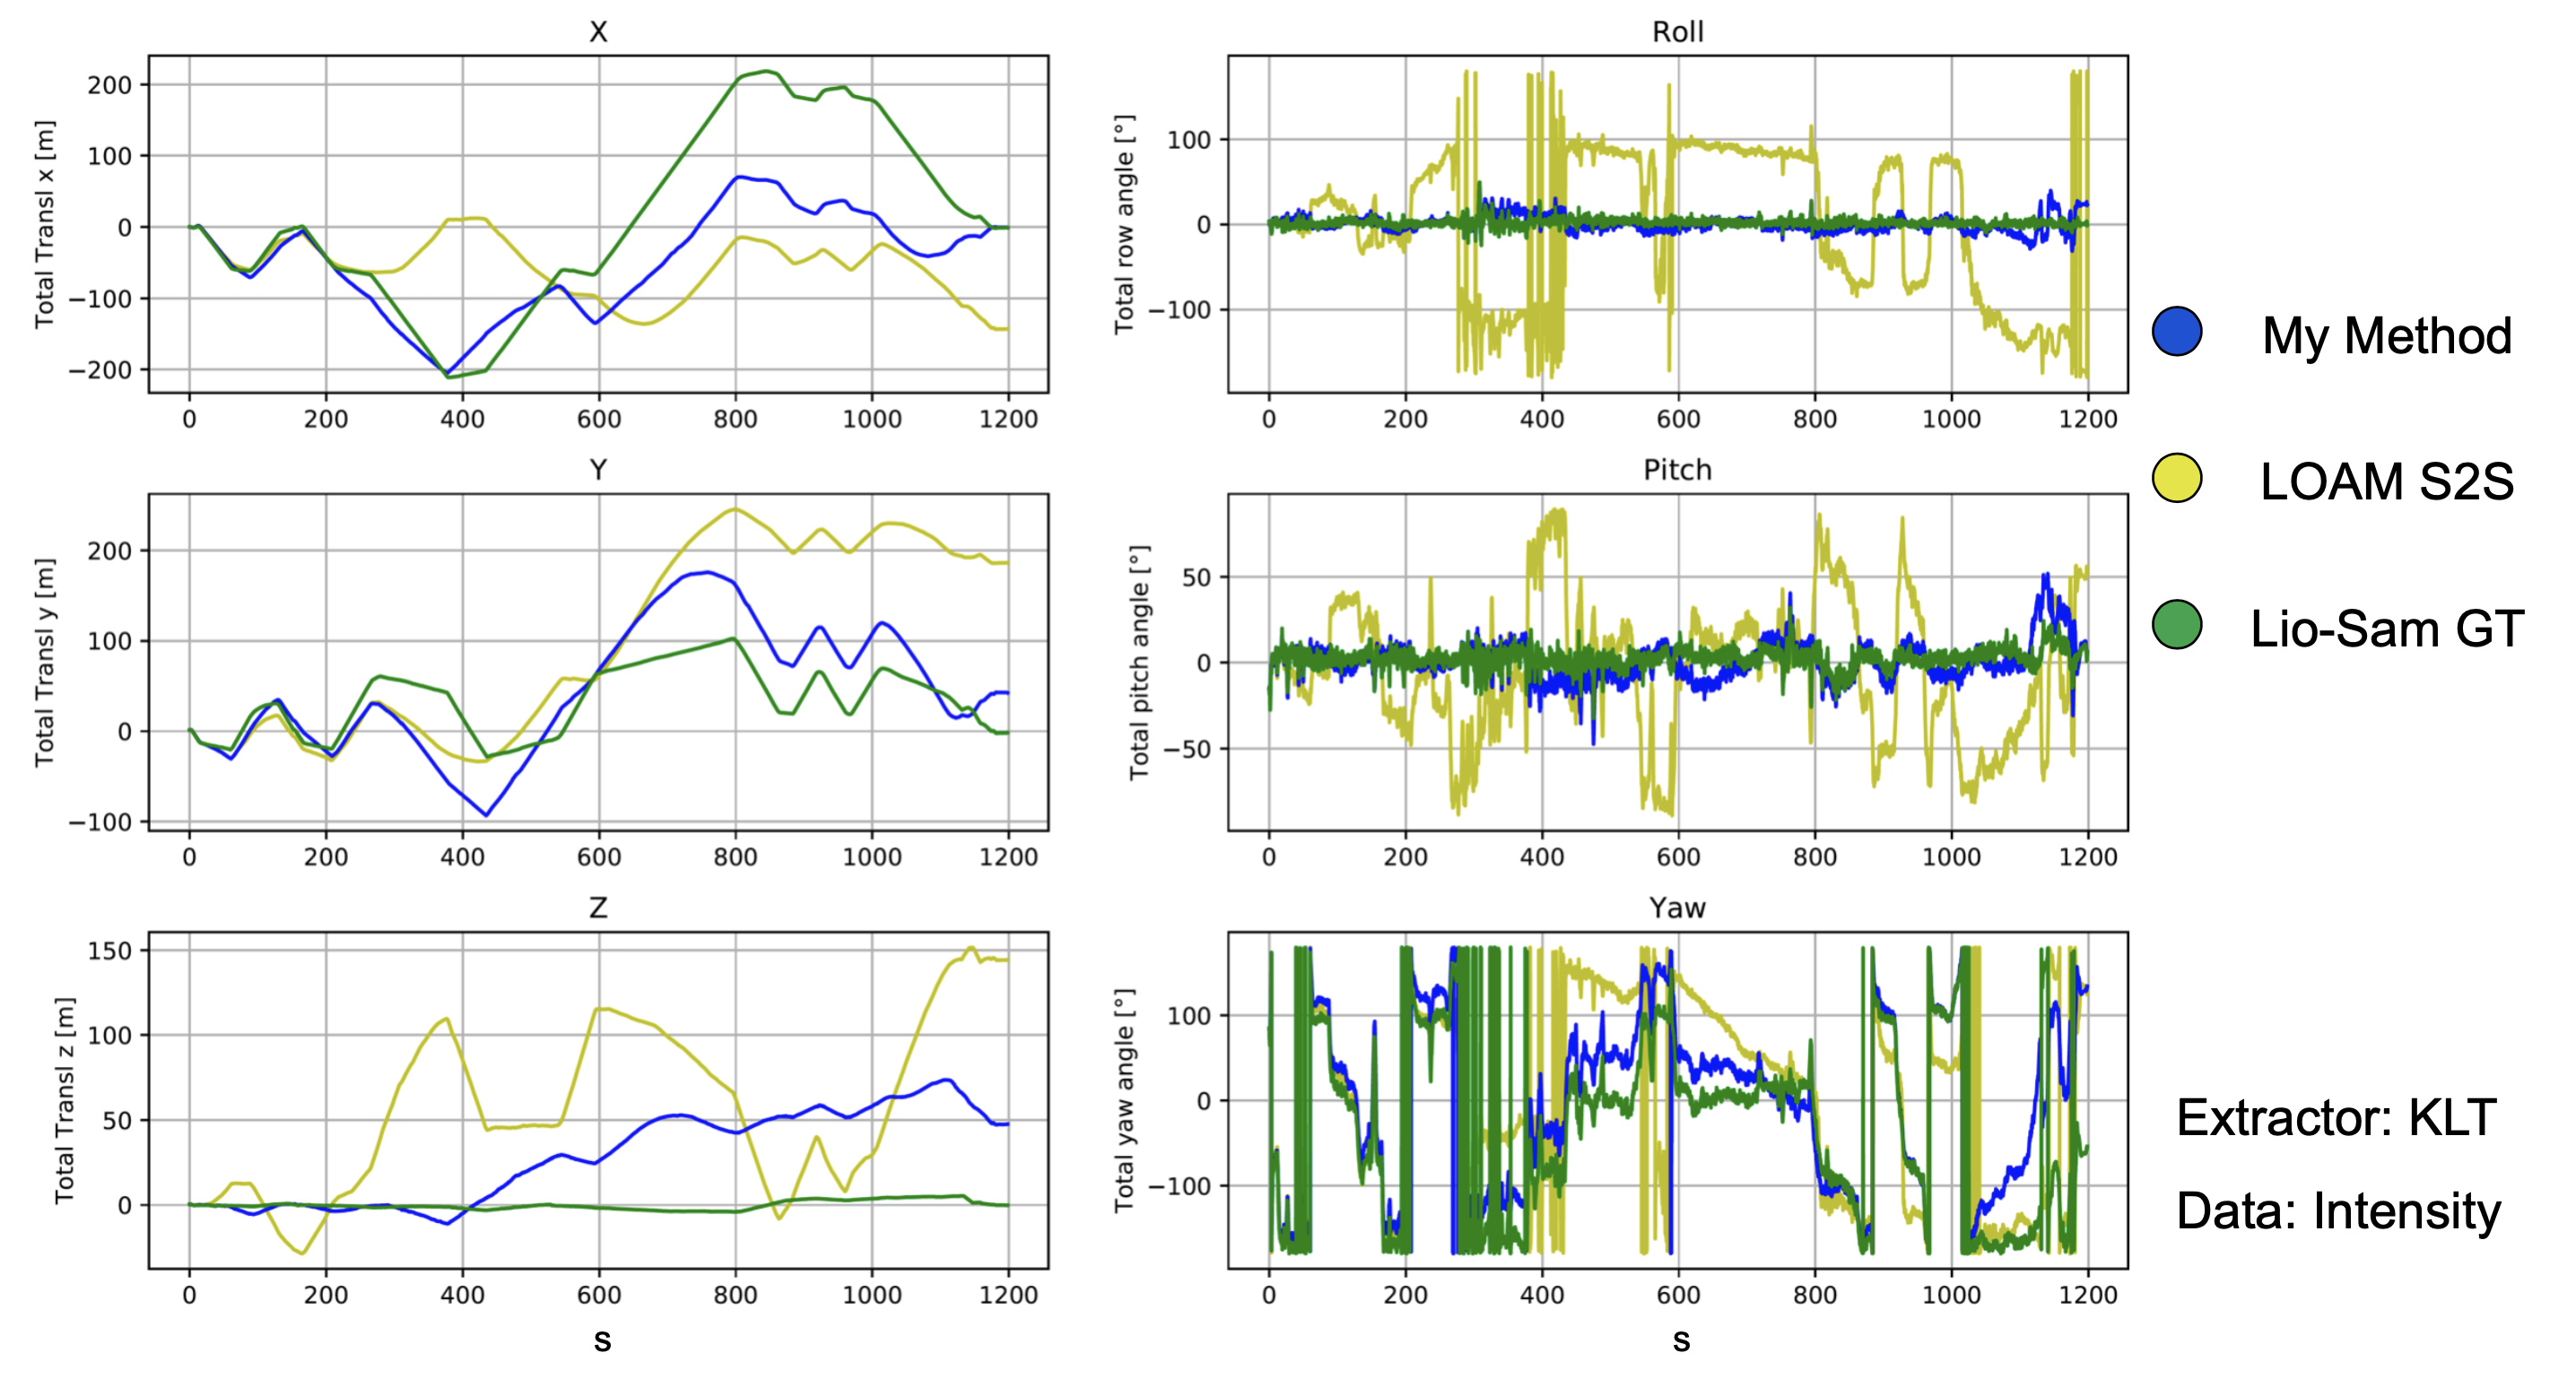
\includegraphics[scale = 0.25]{images/results/pose_klt.png}
%             \caption{Pose comparison}
%             \label{fig:pose_comparison_klt}
%         \end{figure}

%         \begin{figure}[ht]
%             \centering
%             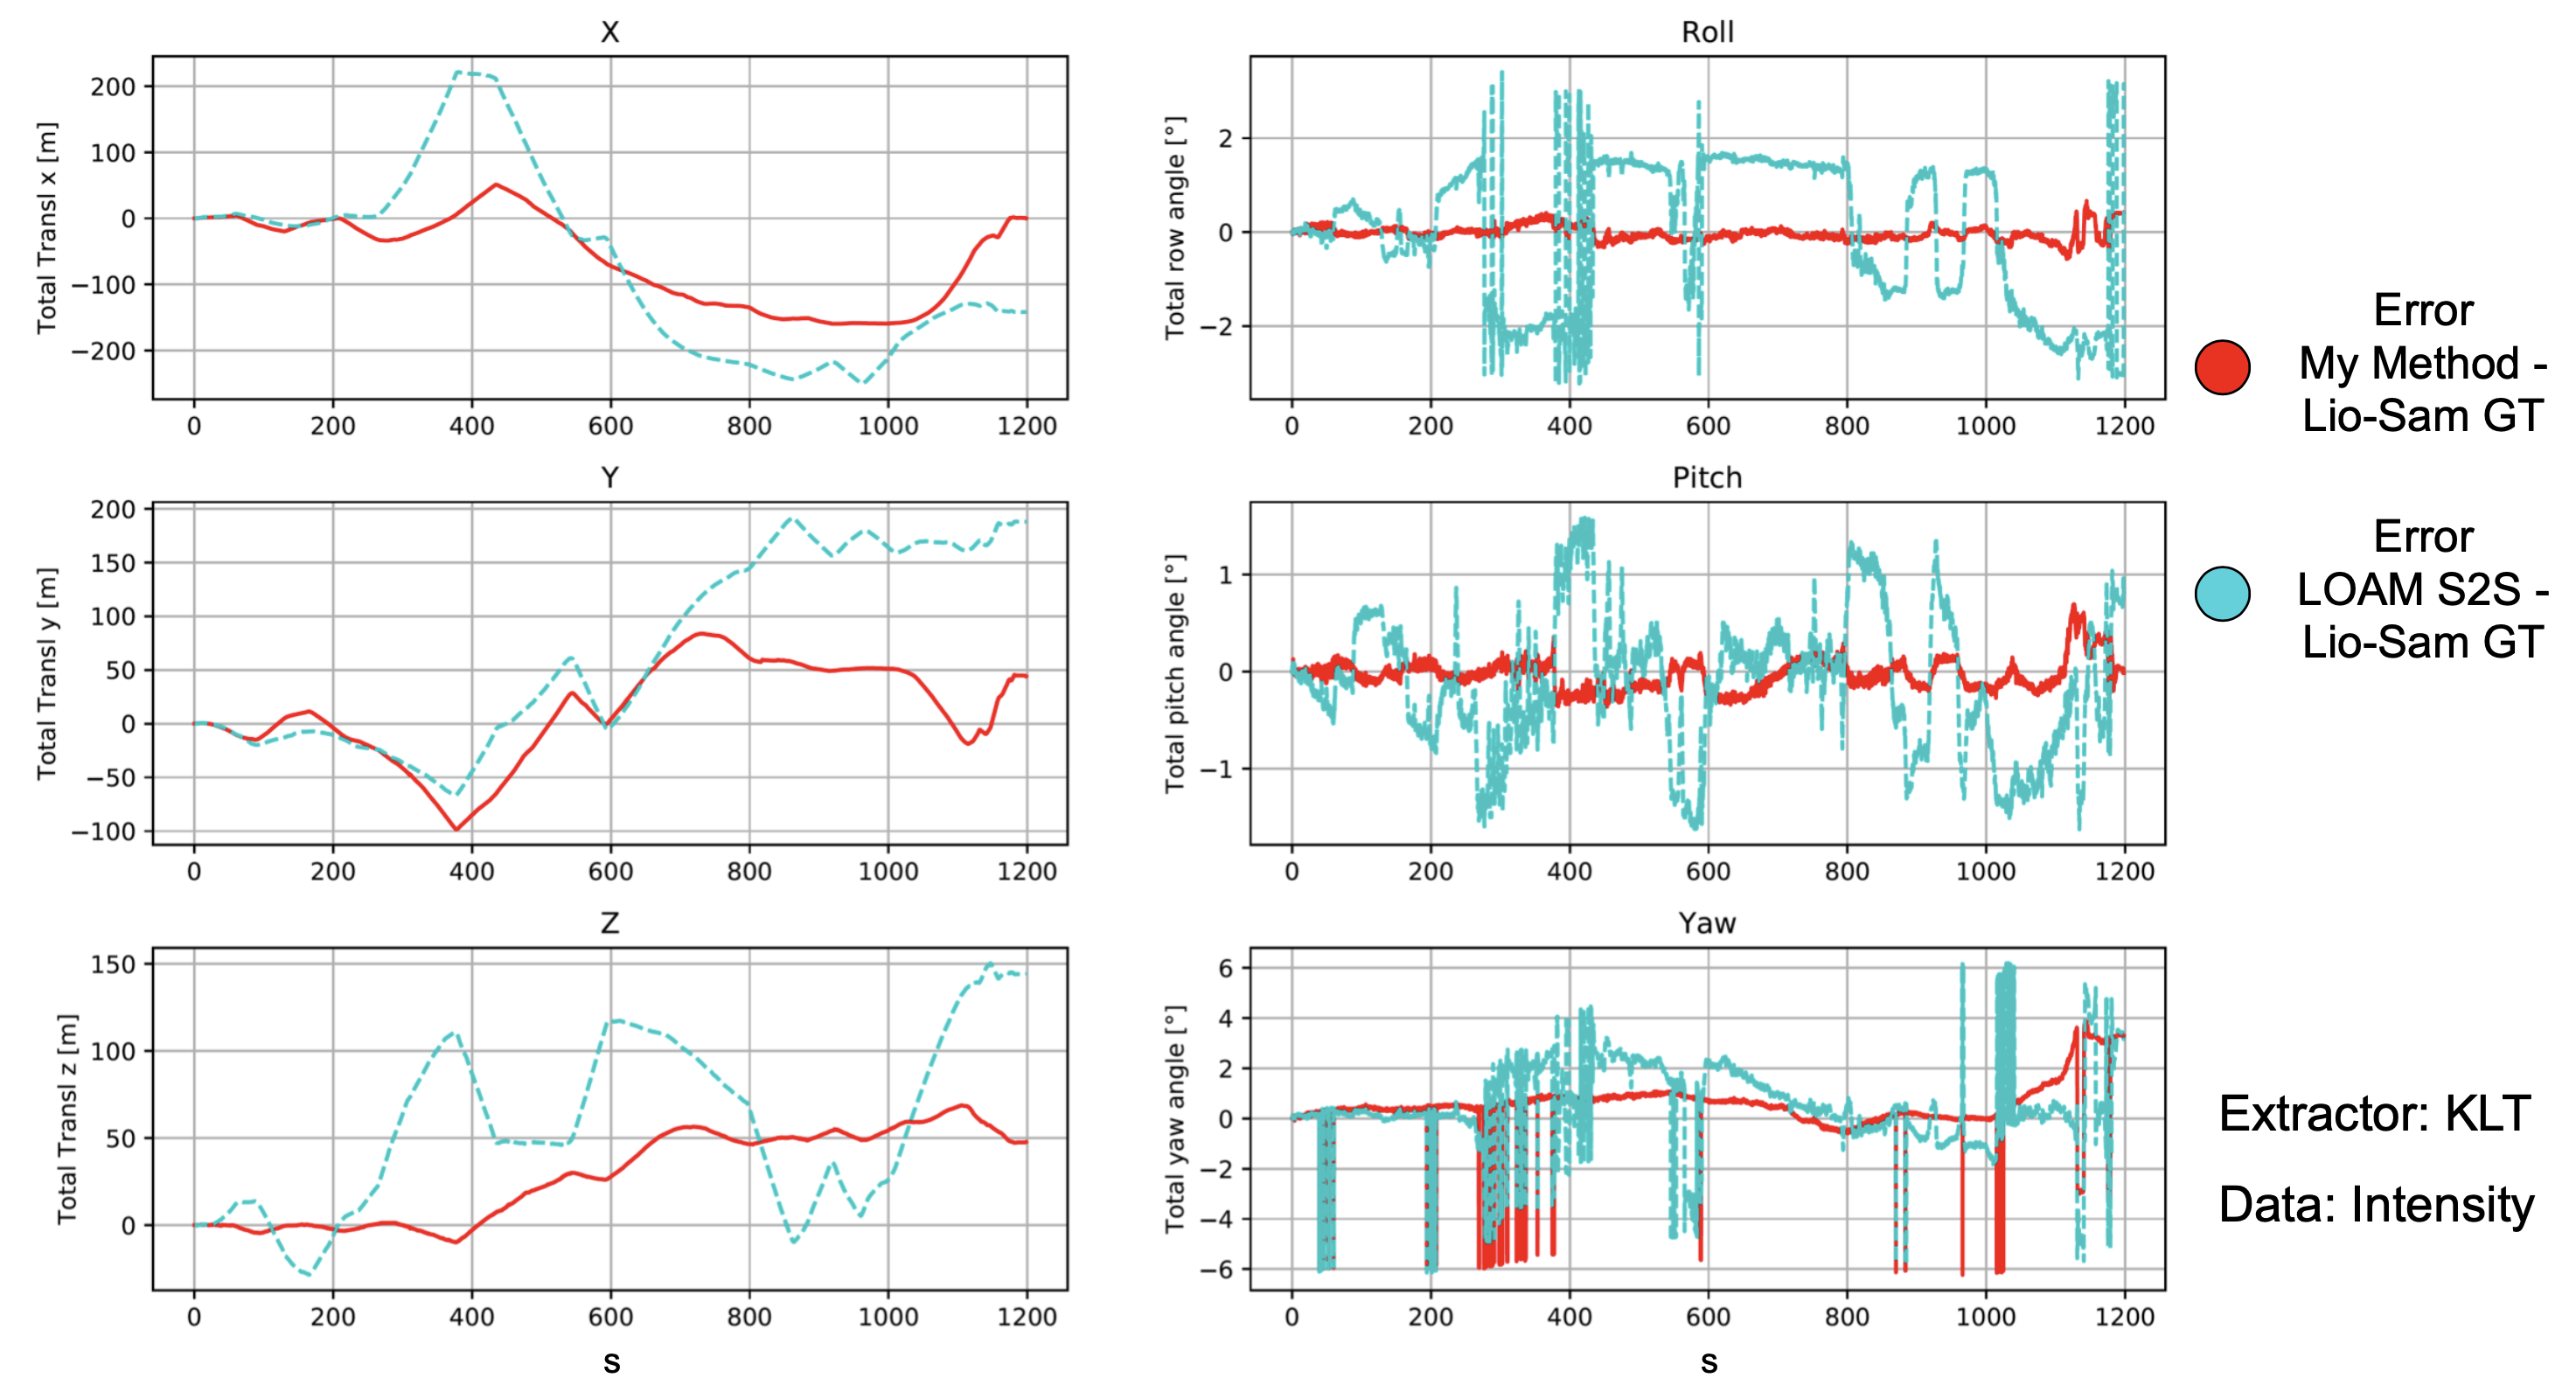
\includegraphics[scale = 0.25]{images/results/pose_error_klt.png}
%             \caption{Pose error comparison}
%             \label{fig:pose_error_comparison_klt}
%         \end{figure}

%         Here in \cref{fig:pose_comparison_klt} and \cref{fig:pose_error_comparison_klt} we can see substantially better global performance of this works method especially regarding the angular development.

%     }

%     \subsection{Comparison of Global Error}{
%         \begin{figure}[ht]
%             \centering
%             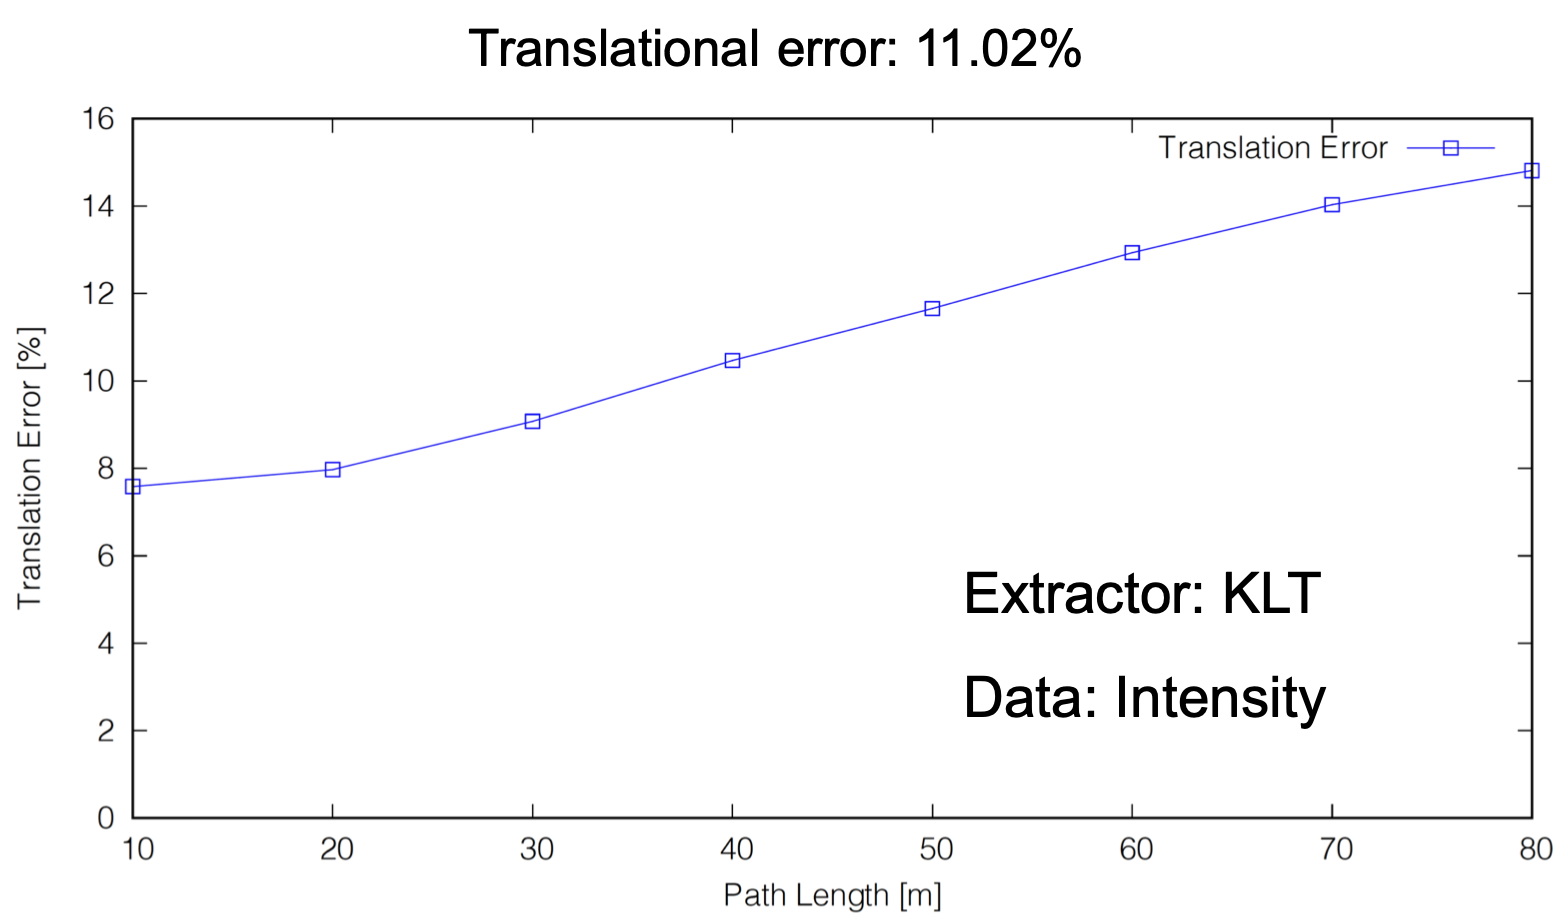
\includegraphics[scale = 0.45]{images/results/mm_drift_translation.png}
%             \caption{My methods translational drift}
%             \label{fig:mm_drift_transl_klt}
%         \end{figure}
        
%         \begin{figure}[ht]
%             \centering
%             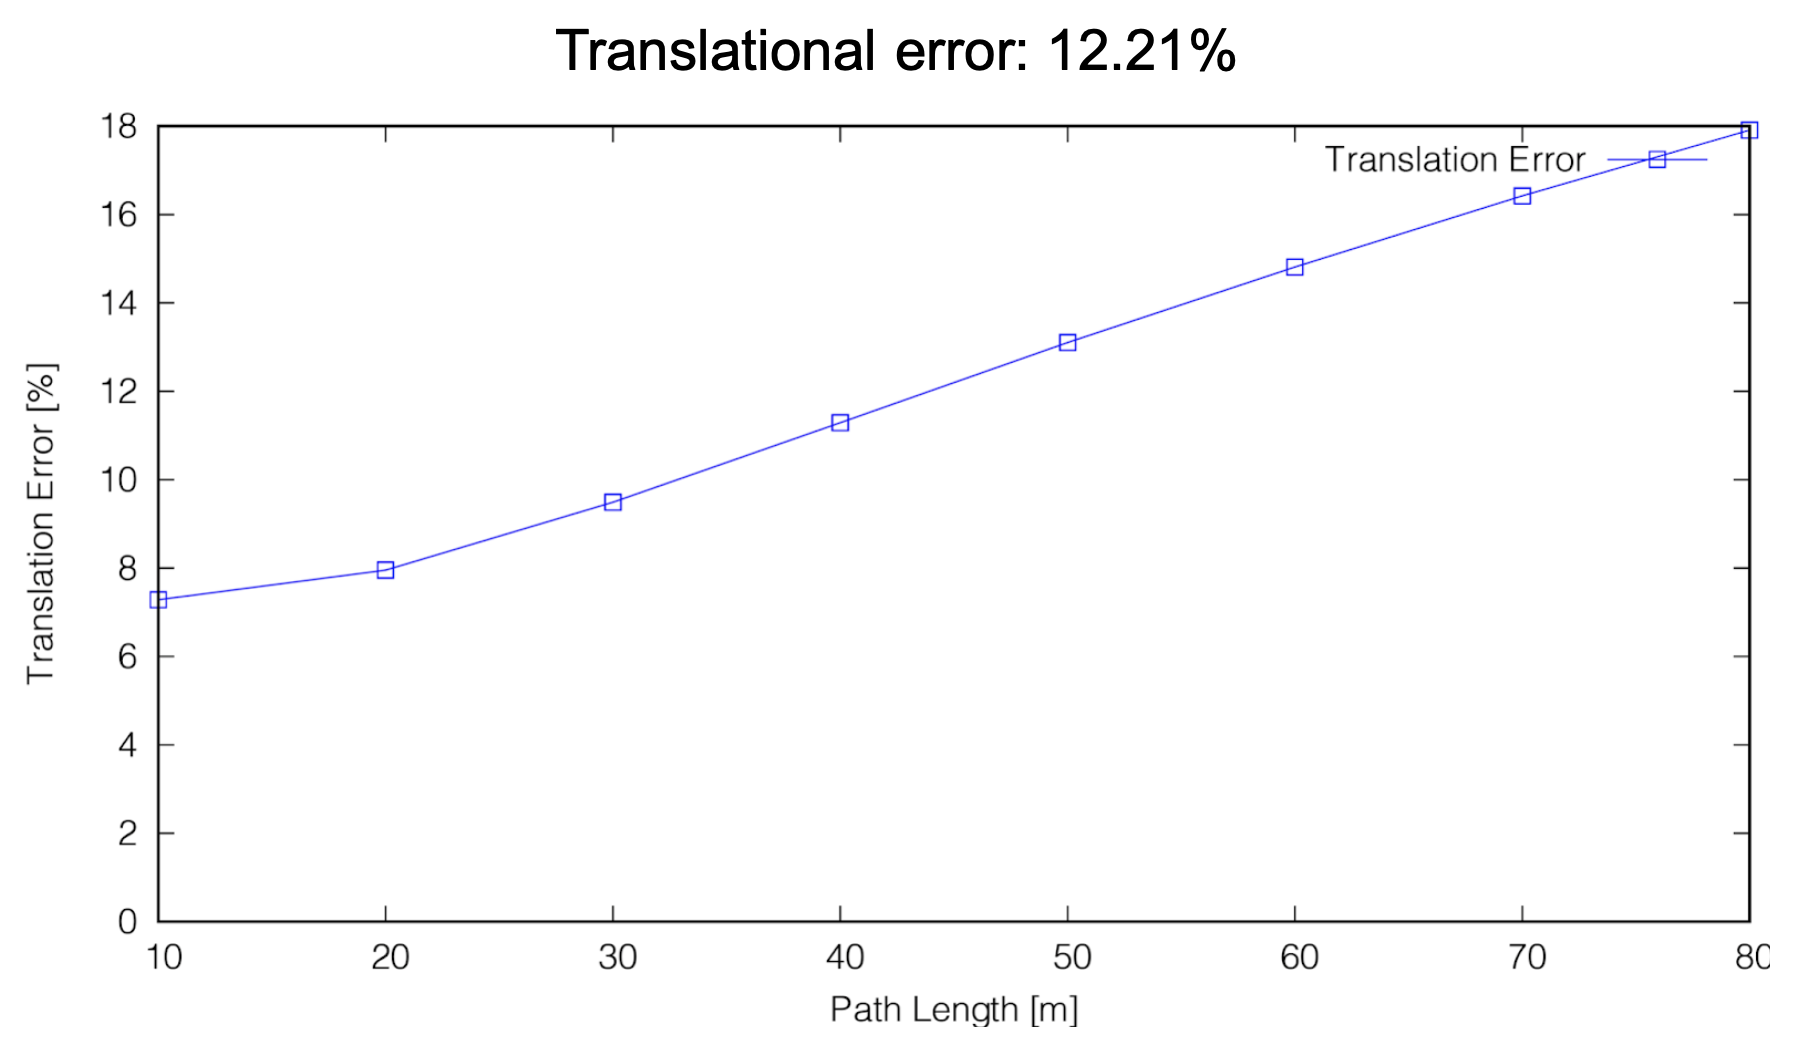
\includegraphics[scale = 0.4]{images/results/loam_drift_transl.png}
%             \caption{LOAM translational drift}
%             \label{fig:loam_drift_transl_klt}
%         \end{figure}
        
%         To account for the drift of the motion estimation a comparison was done after predetermined distance intervals. Here in \cref{fig:mm_drift_transl_klt} to \cref{fig:loam_drift_transl_klt} are the values for the intervals from 10 to 80 meters. It has to be noted that 80 meters is quite a distance and the results from that margin onwards might be slightly deceiving compared to more solid smaller intervals. 
        
%         Averaged over all interval sizes my methods performs a little better as can be seen from the averaged translational error denoted at the top.

%         \clearpage

%         \begin{figure}[ht]
%             \centering
%             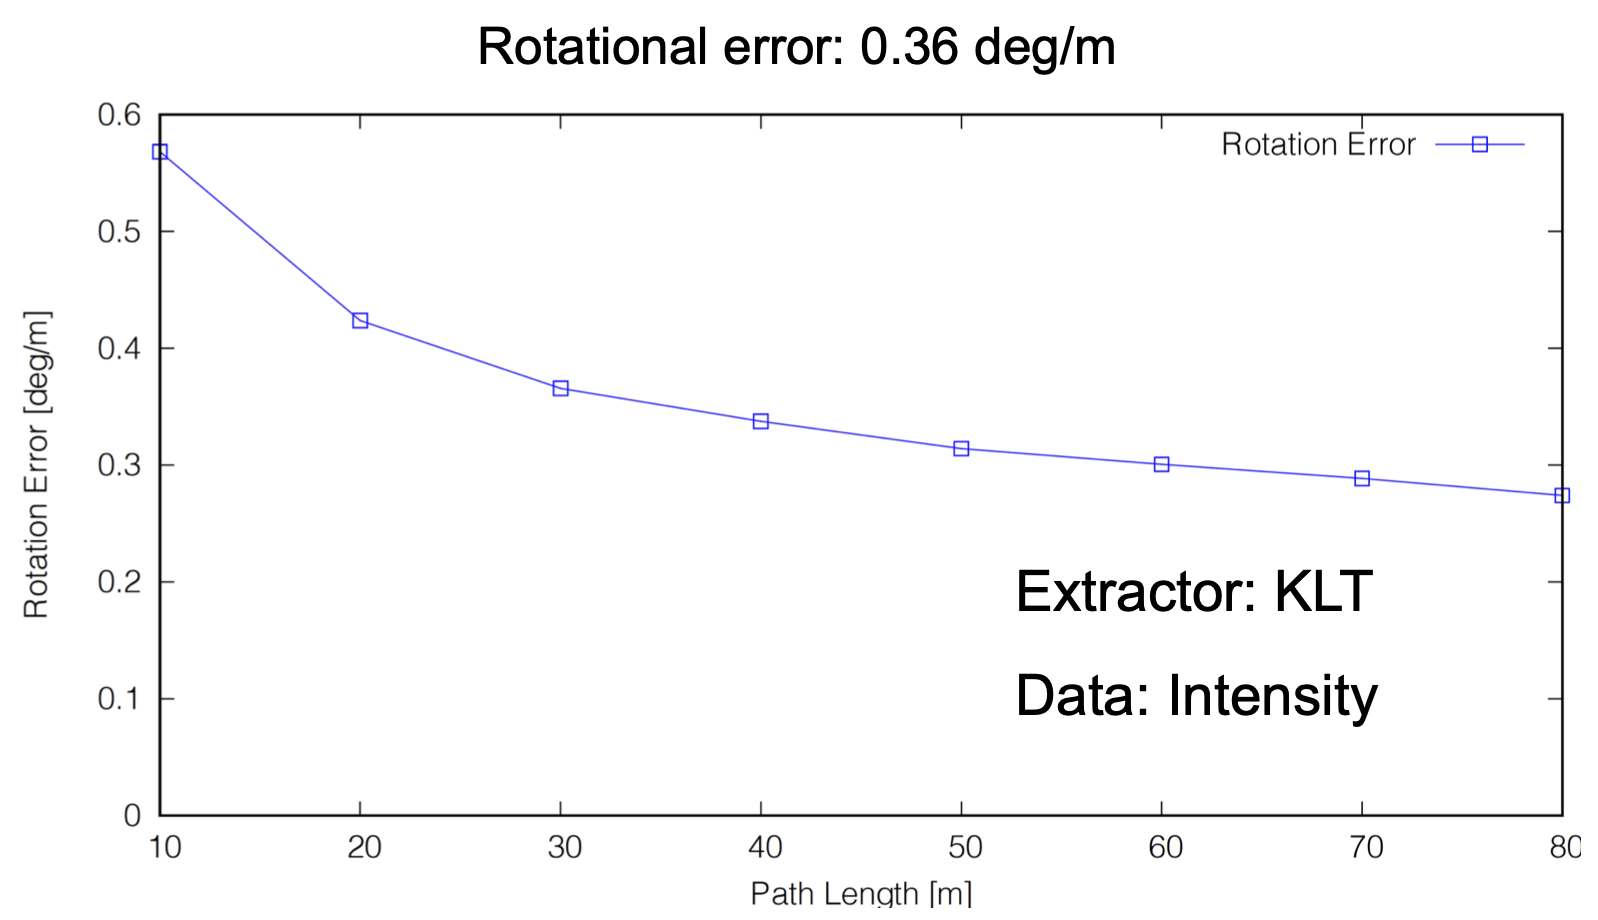
\includegraphics[scale = 0.45]{images/results/mm_drift_angle.png}
%             \caption{My methods angular drift}
%             \label{fig:mm_drift_angle_klt}
%         \end{figure}

%         \begin{figure}[!ht]
%             \centering
%             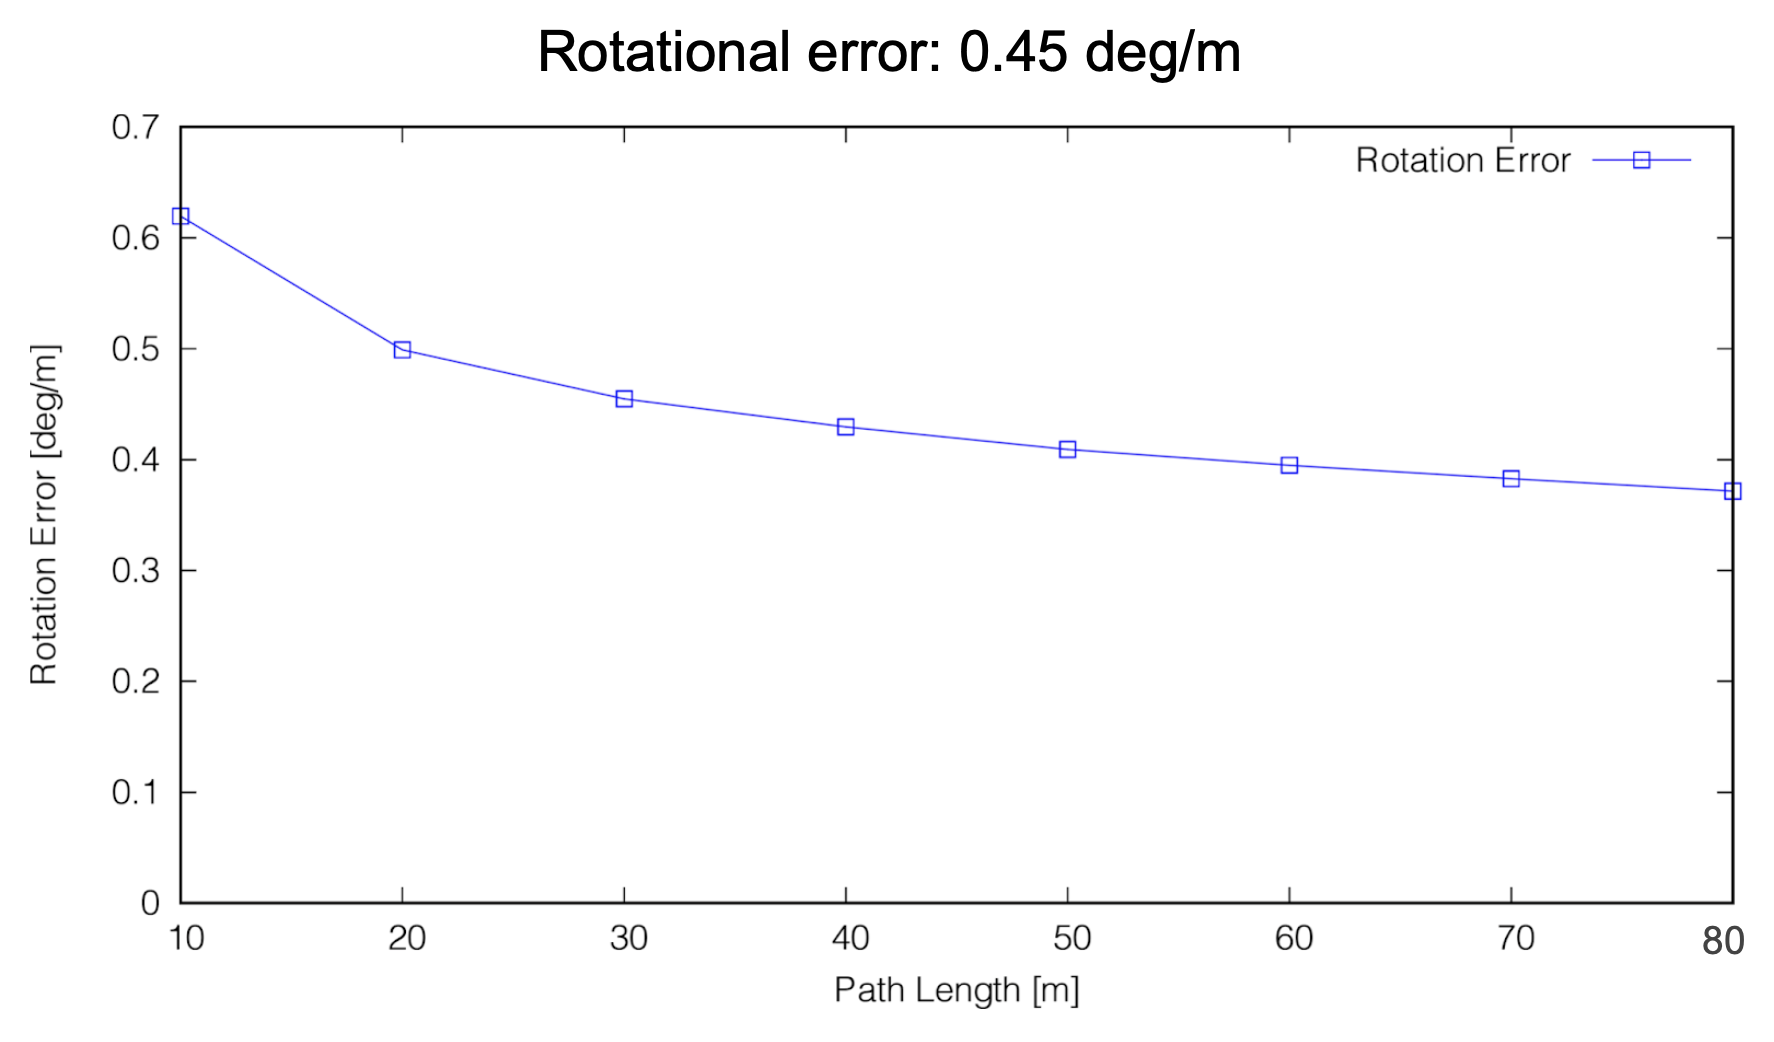
\includegraphics[scale = 0.4]{images/results/loam_drift_angle.png}
%             \caption{loam angular drift}
%             \label{fig:loam_drift_angle_klt}
%         \end{figure}

%         A similar result can be drawn from the angular development. This papers method shows with 0.35 degrees/meter a better performance than the LOAM scan to scan method.
%     }
%     \clearpage

%     \subsection{Comparing Estimated Trajectories}{
%         \begin{figure}[!ht]
%             \centering
%             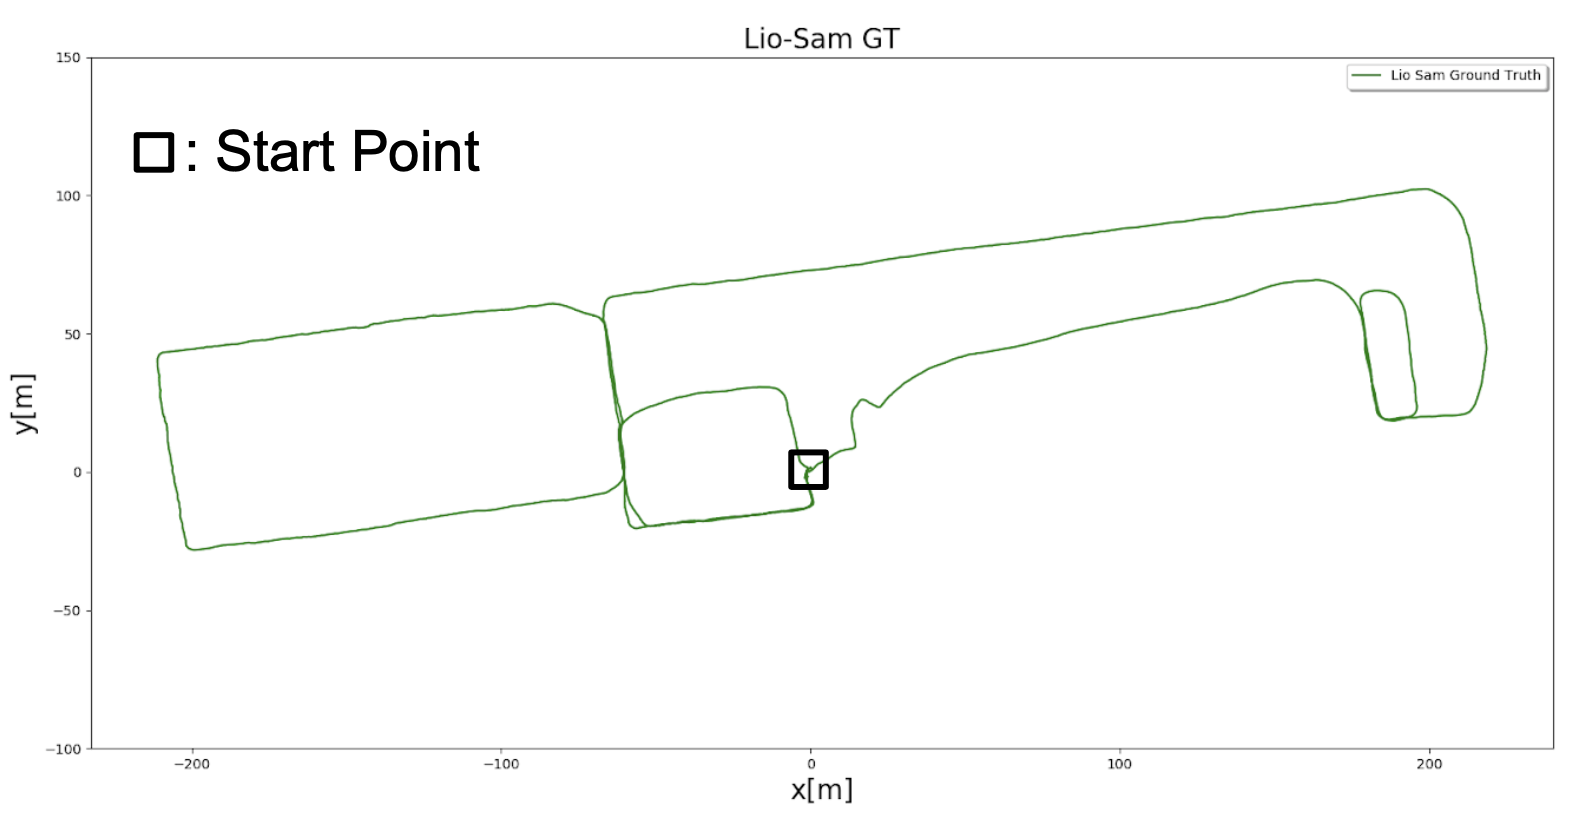
\includegraphics[scale = 0.45]{images/results/GT_trajectory.png}
%             \caption{GT trajectory}
%             \label{fig:GT_trajectory}
%         \end{figure}

%         Indicated on the plot above is the datasets trajectory estimated by Lio-Sam. This will again be considered the ground truth.

%         \begin{figure}[!ht]
%             \centering
%             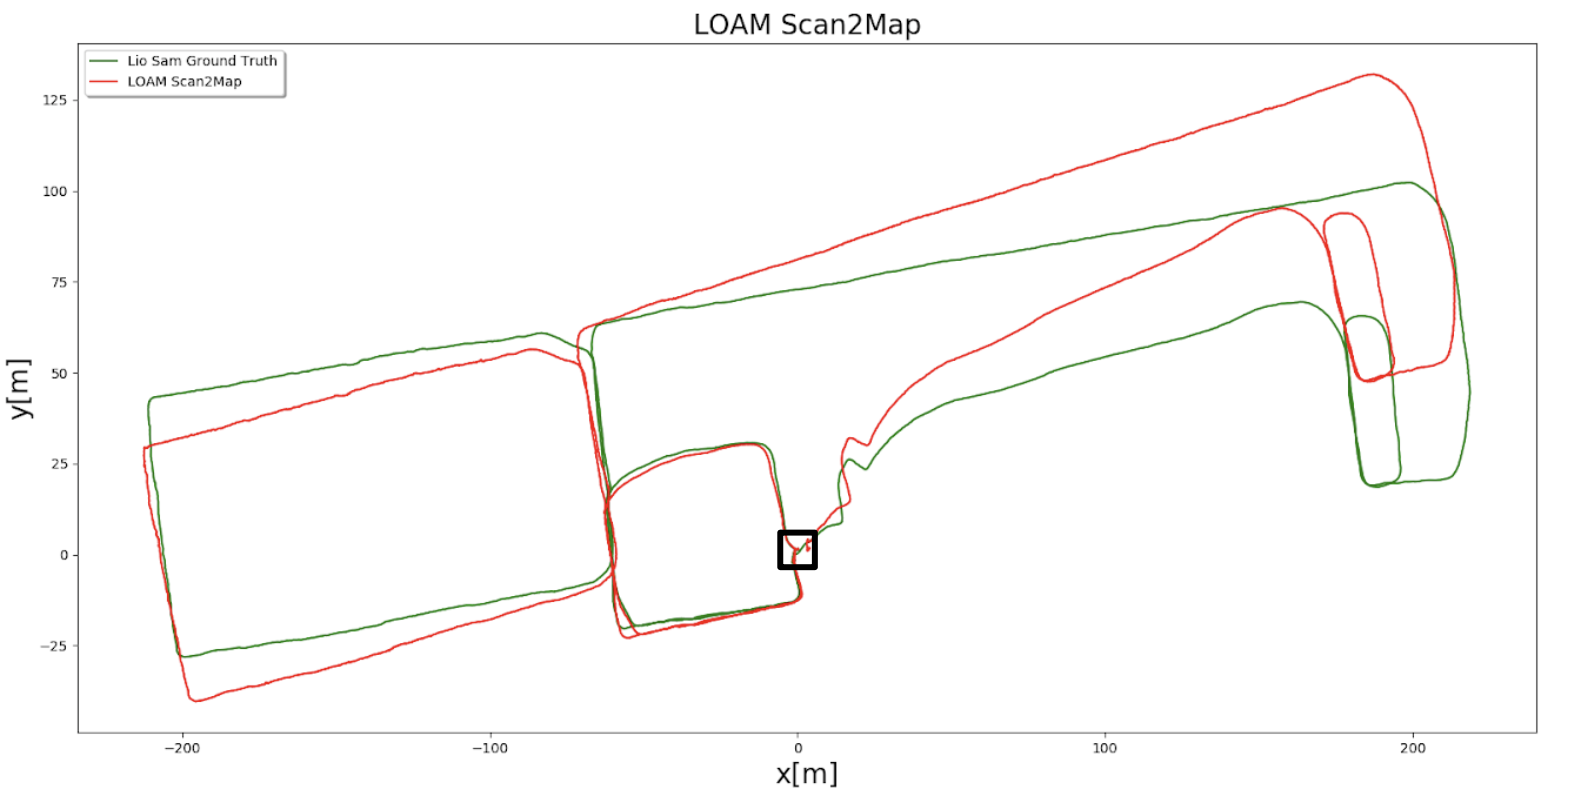
\includegraphics[scale = 0.45]{images/results/loam_s2m_trajectory.png}
%             \caption{LOAM scan to map trajectory}
%             \label{fig:loam_s2m_trajectory}
%         \end{figure}

%         As aforementioned the LOAM method performs very well as it is also map based and thus really accurate.
%         \clearpage

%         \begin{figure}[!ht]
%             \centering
%             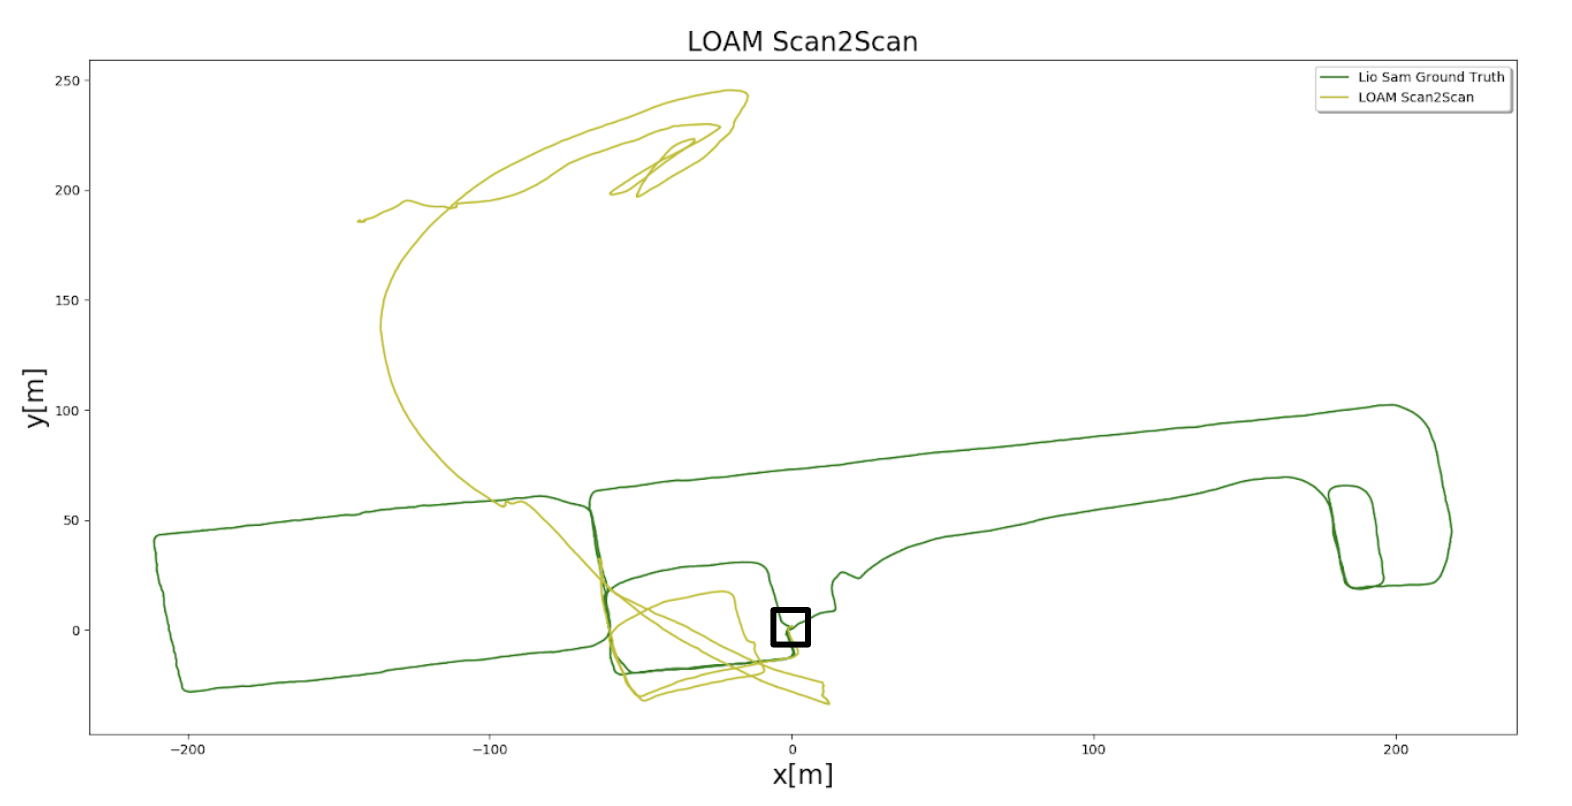
\includegraphics[scale = 0.45]{images/results/loam_s2s_trajectory.png}
%             \caption{LOAM scan to scan trajectory}
%             \label{fig:loam_s2s_trajectory}
%         \end{figure}

%         Considering the solely scan based LOAM estimation it looks quite poor.

%         \begin{figure}[!ht]
%             \centering
%             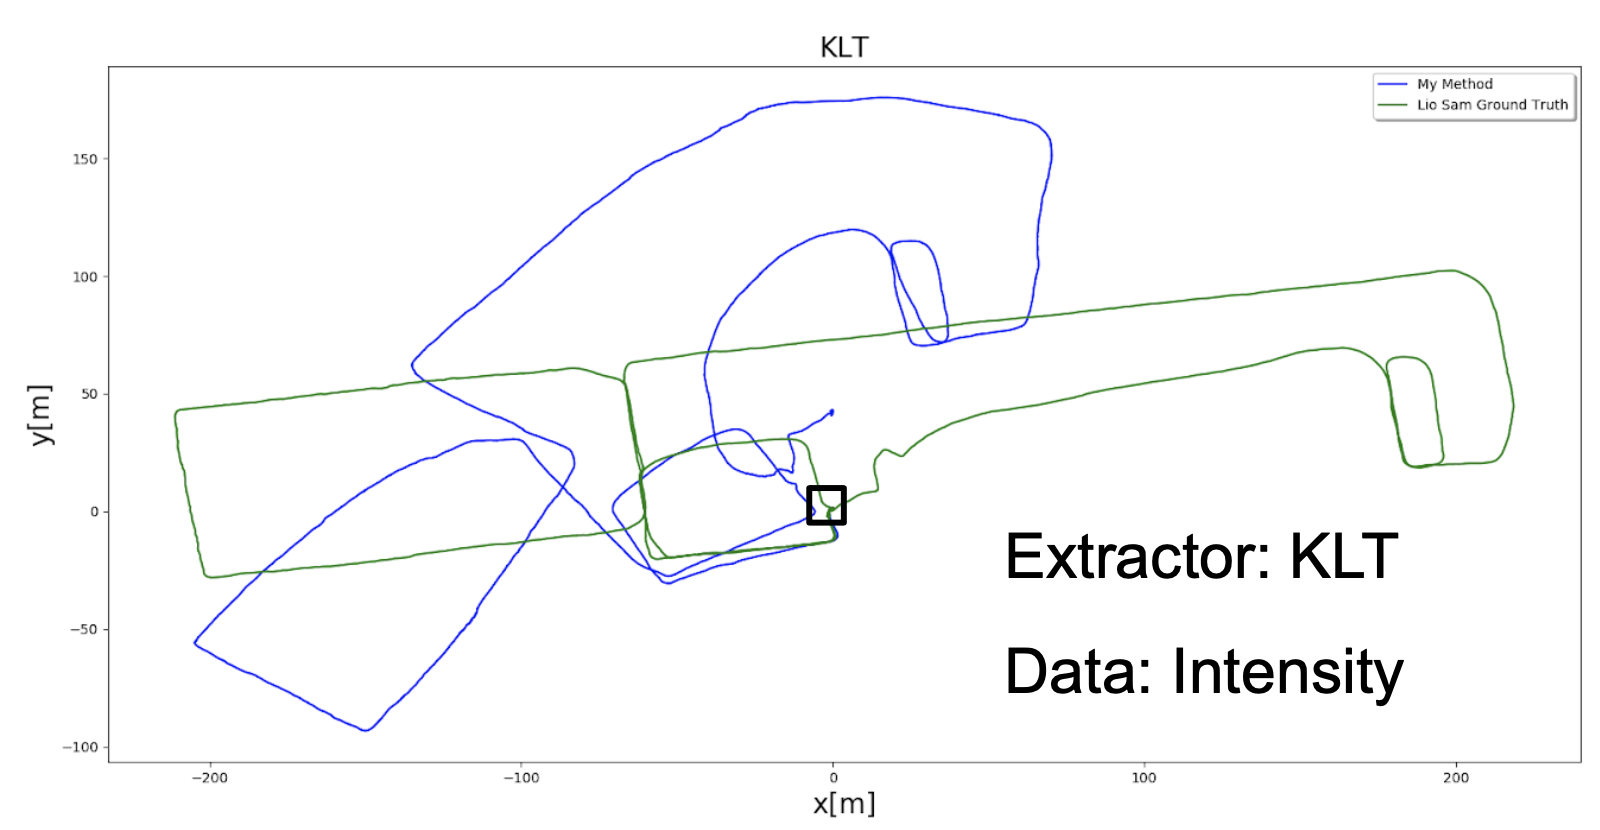
\includegraphics[scale = 0.45]{images/results/mm_trajectory.png}
%             \caption{This works methods trajectory}
%             \label{fig:mm_trajectory}
%         \end{figure}

%         When looking at method from this paper it does accumulate quite some drift but performs considerably better than the scan based LOAM implementation. For additional performance results of this method consult \cref{sec:additional_results}
%     }
%     \clearpage
% }

    
% \section{Final Comparison of Feature Methods}{
%         In this section I will perform a comparison of the feature methods to the point of a possible verdict. For in depth data about each respective method consult \cref{ch:additional_plots}

%         \subsection{Local Step Comparison – feature methods}{

%         \begin{tabular}{p{2cm} p{3.5cm} p{3.7cm} p{2cm}}
%             & \textbf{ORB} & \textbf{BRISK} & \textbf{KLT}
%         \end{tabular}

%         \begin{table}[!ht]
%             \setlength{\extrarowheight}{5pt}
%             \centering
%             \large
%             \begin{tabular}{p{1.3cm}| p{1.5cm} p{1.5cm}| p{1.5cm} p{1.5cm}| p{1.5cm} p{1.5cm}}
%                 \hline
%                 \textbf{Errors} & Mean & STD & Mean & STD & Mean & STD\\[12pt]
%                 \hline
%                 X[m] & -0.004 & 0.056 & 0.004 & 0.219 & \text{\color{Green}{-0.003}} & \text{\color{Cyan}{0.048}}\\[3pt]
%                 \hline
%                 Y[m] & \text{\color{Green}{0}} & 0.040 & \text{\color{Green}{0}} & 0.117 & 0.001 & \text{\color{Cyan}{0.035}}\\[3pt]
%                 \hline
%                 Z[m] & -0.001 & 0.058 & -0.001 & 0.097 & \text{\color{Green}{0}} & \text{\color{Cyan}{0.046}}\\[3pt]
%                 \hline
%                 Roll[°] & \text{\color{Green}{0}} & \text{\color{Cyan}{0.024}} & 0.001 & 0.049 & \text{\color{Green}{0}} & 0.025\\[3pt]
%                 \hline
%                 Pitch[°] & \text{\color{Green}{0}} & \text{\color{Cyan}{0.024}} & \text{\color{Green}{0}} & 0.028 & \text{\color{Green}{0}} & \text{\color{Cyan}{0.024}}\\[3pt]
%                 \hline
%                 Yaw[°] & \text{\color{Green}{0}} & \text{\color{Cyan}{0.024}} & \text{\color{Green}{0}} & 0.048 & \text{\color{Green}{0}} & 0.029\\[3pt]
%             \end{tabular}
%             \caption{Average Step Error Comparison for Feature Methods}
%             \label{tab:step_errors_methods}
%         \end{table}

%         In \cref{tab:step_errors_methods} we can see the iterative performance of the feature methods. 
        
%         ORB and KLT seem to perform similarly while BRISK falls off a little regarding the standard deviation.

%         }
%         \subsection{Trajectory Comparison – feature methods}{

%         \begin{figure}[!ht]
%             \centering
%             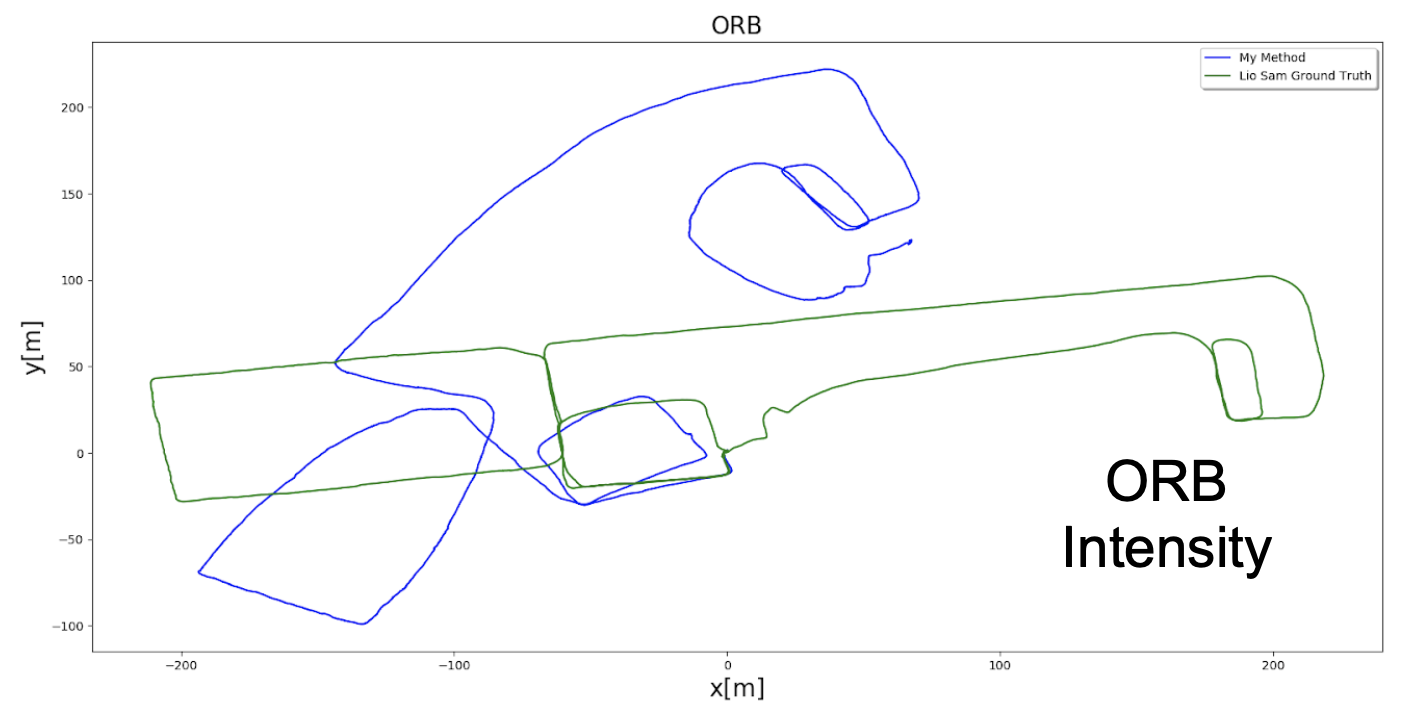
\includegraphics[scale = 0.5]{images/comparison_appendix/ORBt.png}
%             \caption{ORB trajectory}
%             \label{fig:ORB_trajectory}
%         \end{figure}
%         \clearpage

%         \begin{figure}[!ht]
%             \centering
%             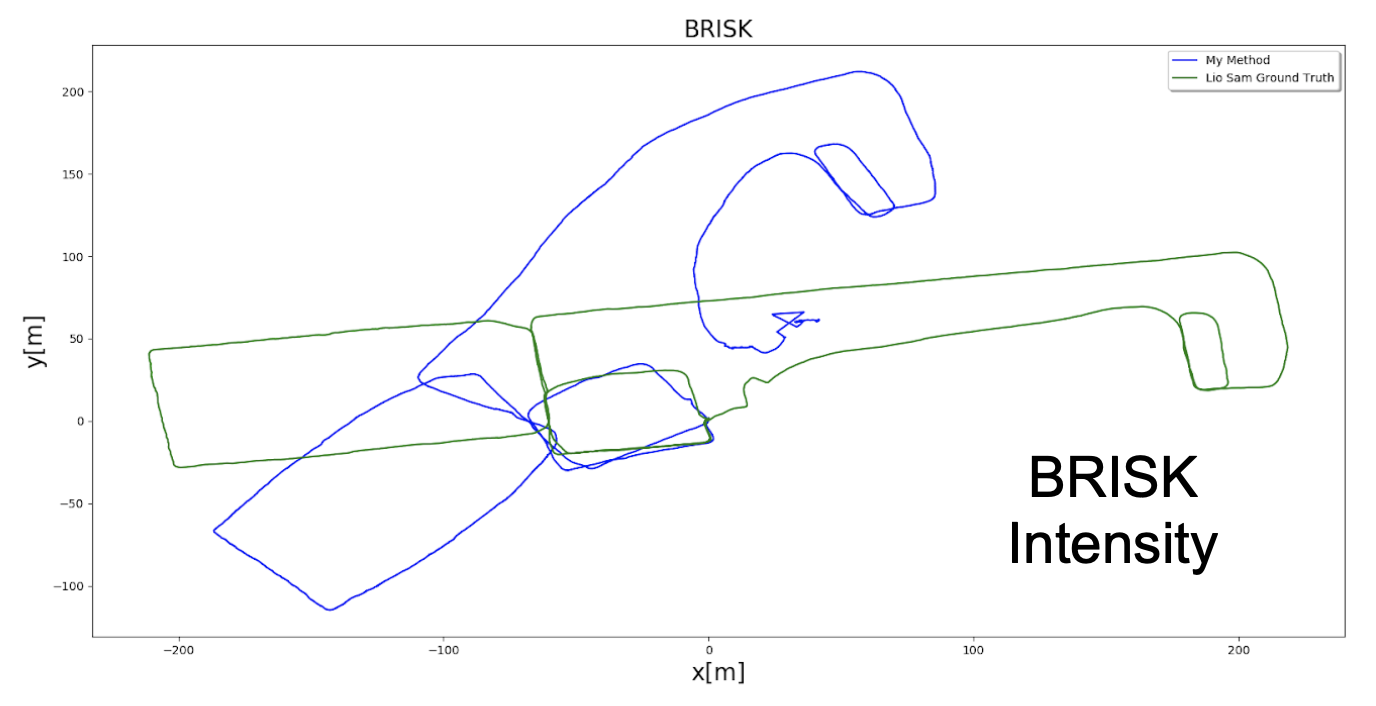
\includegraphics[scale = 0.5]{images/comparison_appendix/BRISKt.png}
%             \caption{BRISK trajectory}
%             \label{fig:BRISK_trajectory}
%         \end{figure}

%         \begin{figure}[!ht]
%             \centering
%             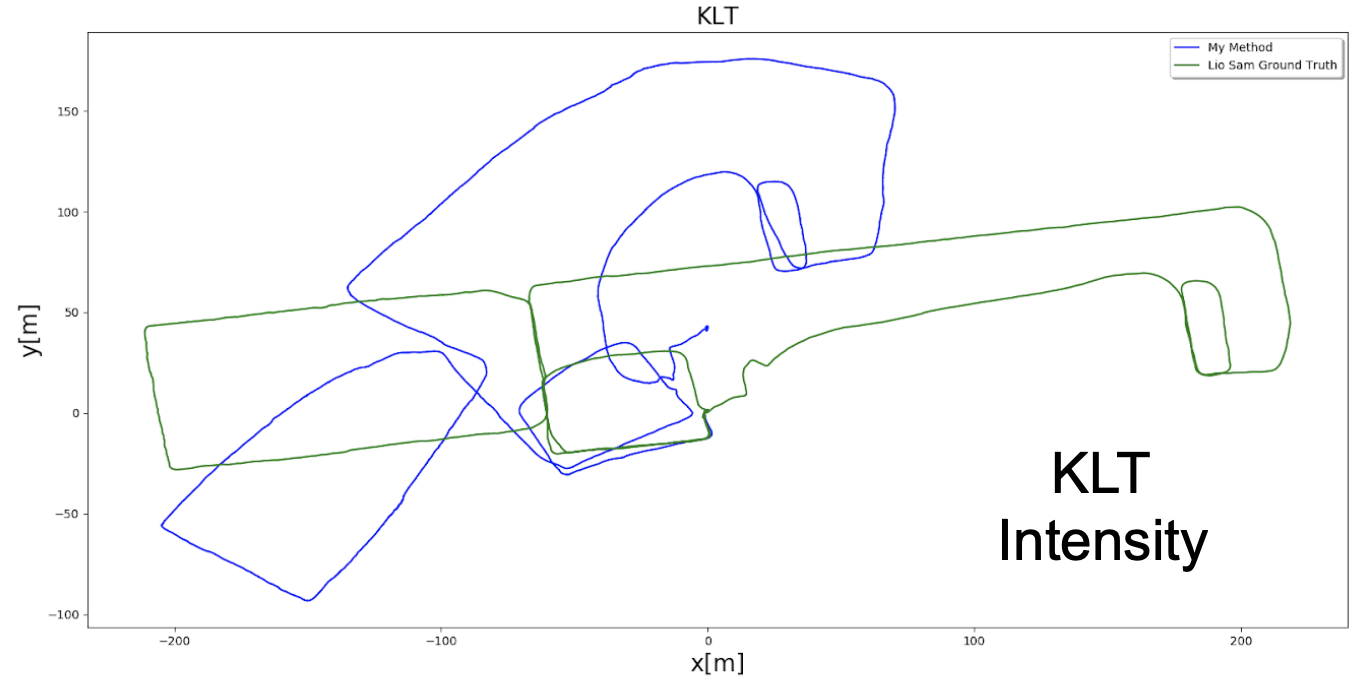
\includegraphics[scale = 0.5]{images/comparison_appendix/KLTt.png}
%             \caption{KLT trajectory}
%             \label{fig:KLT_trajectory_method}
%         \end{figure}
%         }
%         \clearpage
%         \subsection{Drift Comparison – feature methods}{
%             I also compared the more promising methods ORB and KLT regarding the accumulated drift:
%             \subsubsection{Translational Drift - feature methods}{
%                 \begin{figure}[!ht]
%                     \centering
%                     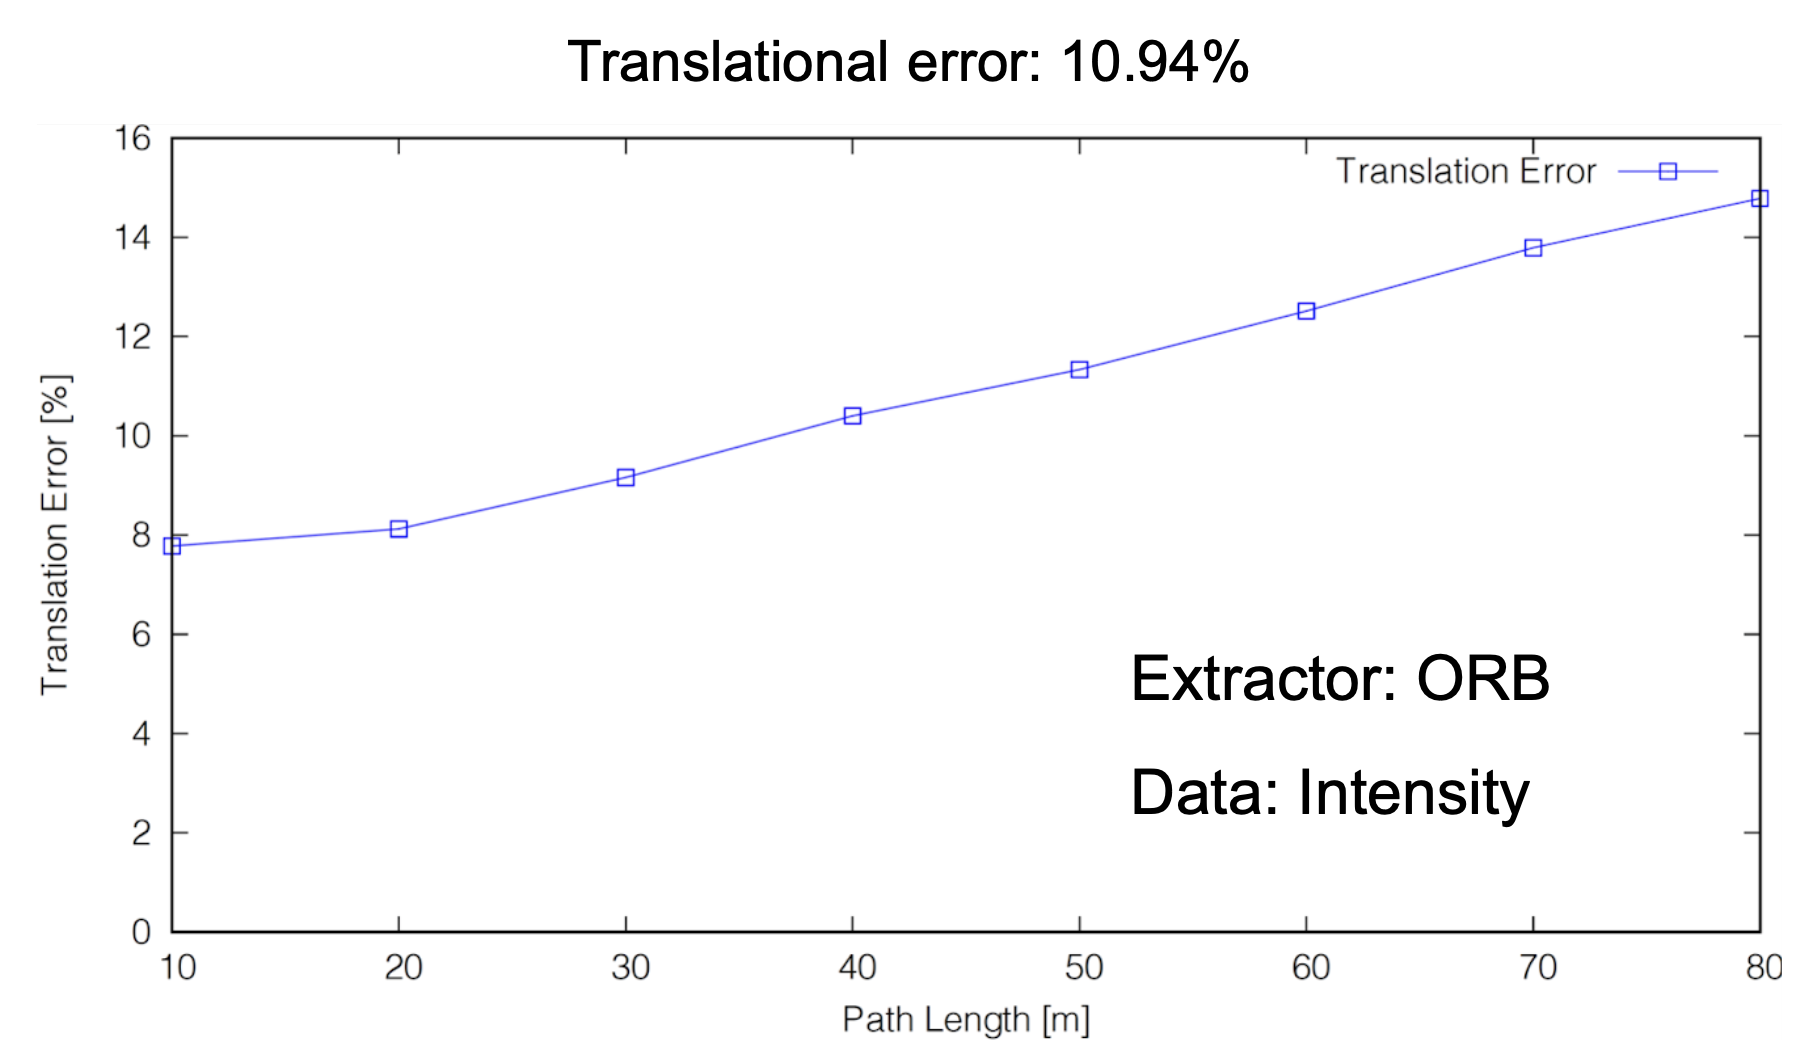
\includegraphics[scale = 0.4]{images/comparison_appendix/orb_drift_transl.png}
%                     \caption{ORB drift translation}
%                     \label{fig:ORB_drift_transl}
%                 \end{figure}

%                 \begin{figure}[!ht]
%                     \centering
%                     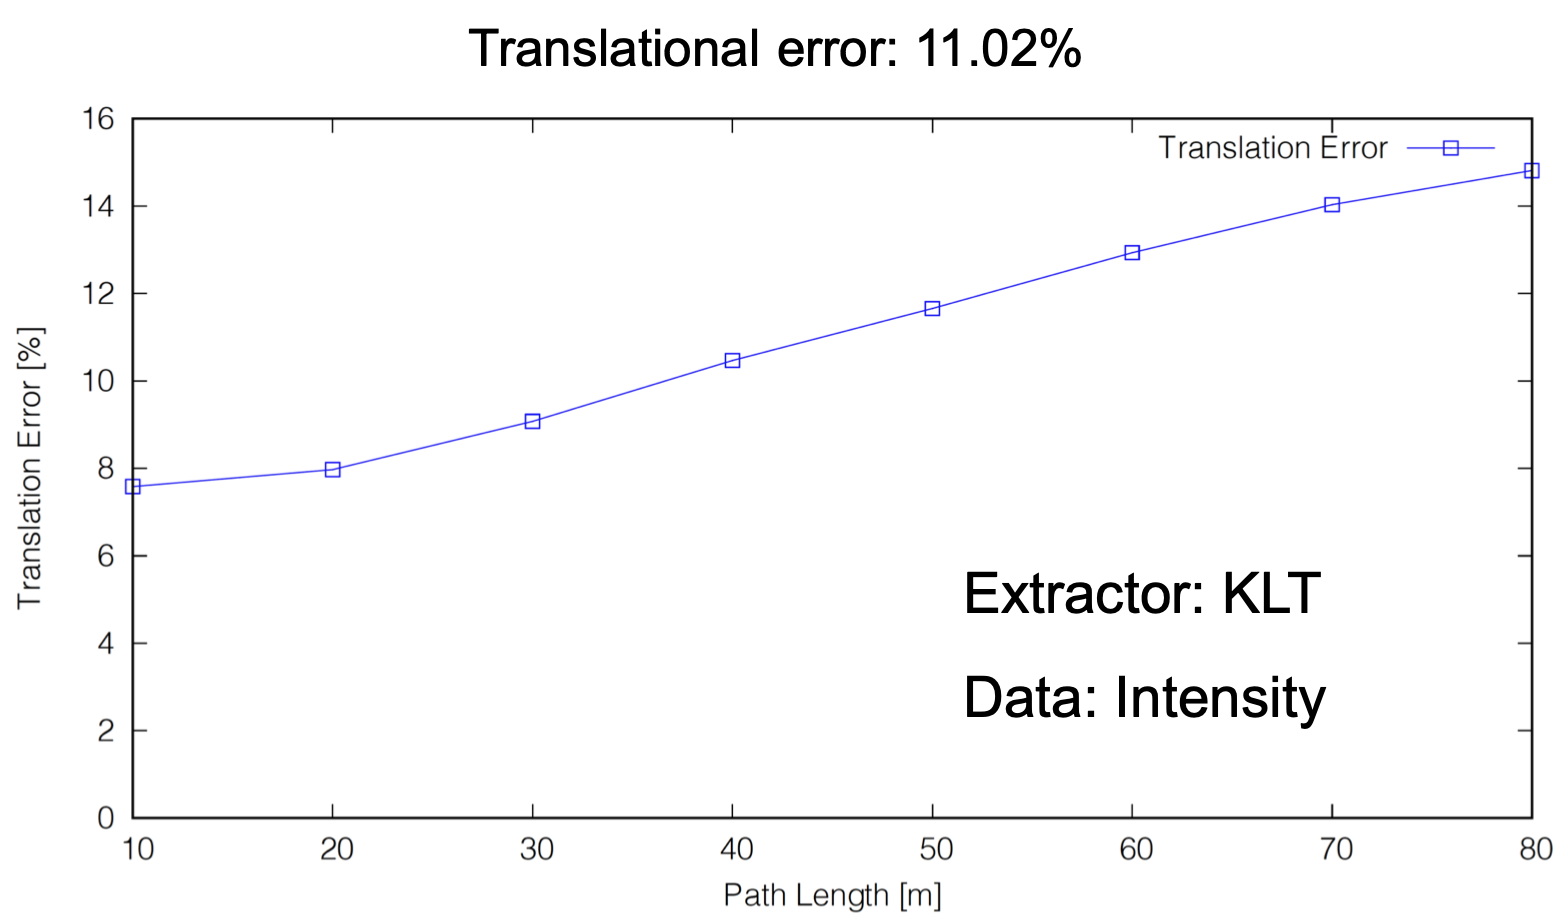
\includegraphics[scale = 0.45]{images/results/mm_drift_translation.png}
%                     \caption{KLT translational drift}
%                     \label{fig:KLT_drift_transl}
%                 \end{figure}
%                     }
%                 \clearpage
%             \subsubsection{Angular Drift - feature methods}{

%                 \begin{figure}[!ht]
%                     \centering
%                     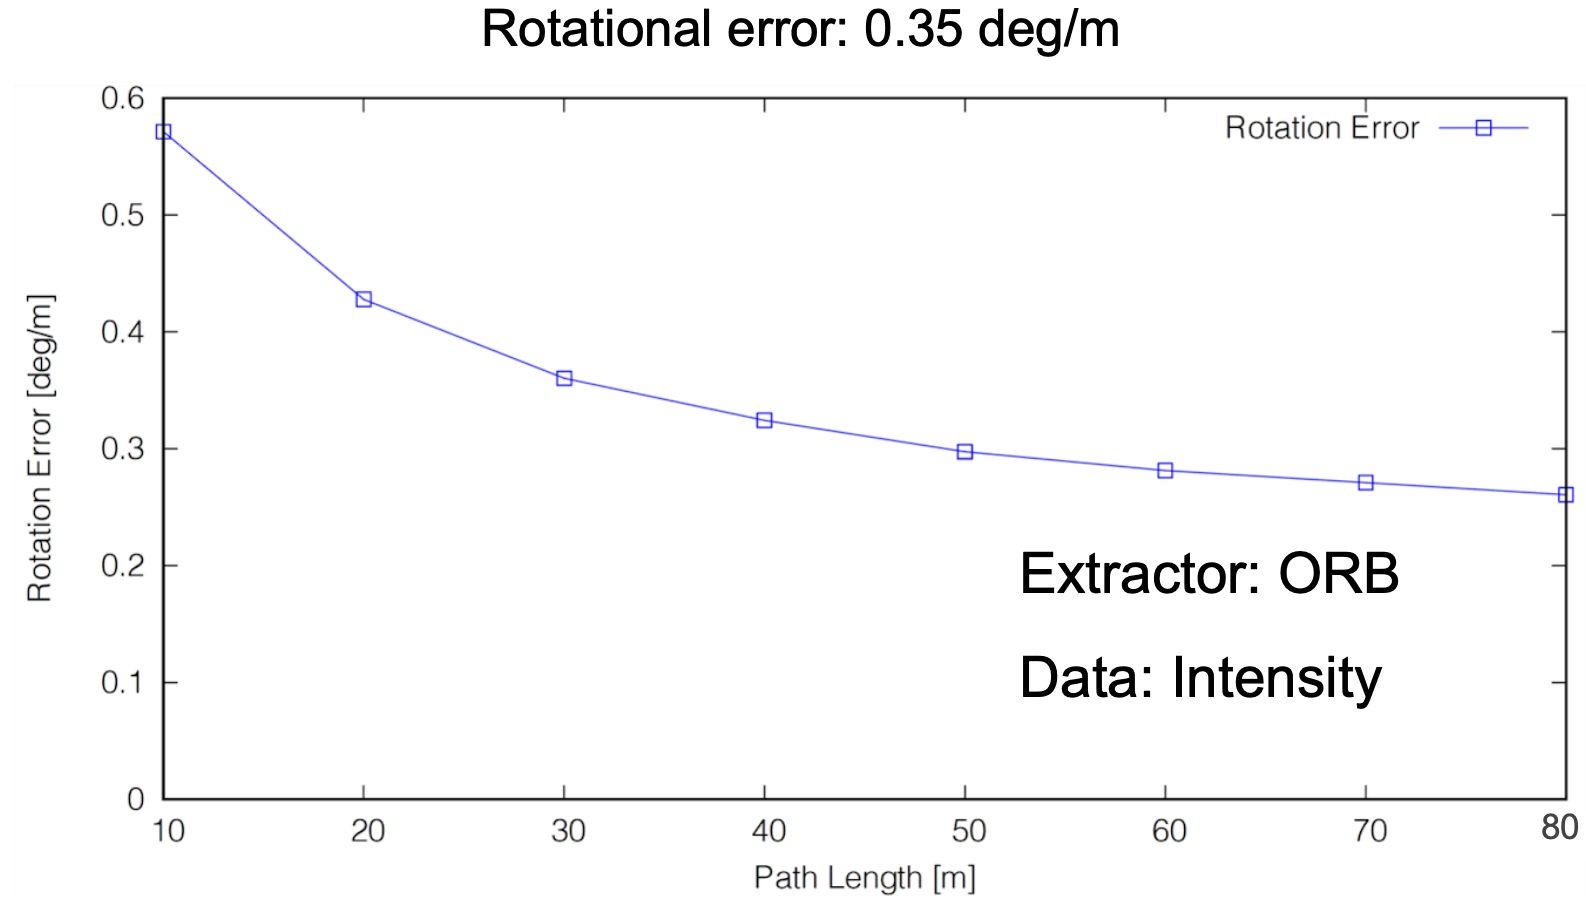
\includegraphics[scale = 0.45]{images/comparison_appendix/orb_drift_angle.png}
%                     \caption{ORB angular drift}
%                     \label{fig:ORB_drift_angle}
%                 \end{figure}

%                 \begin{figure}[!ht]
%                     \centering
%                     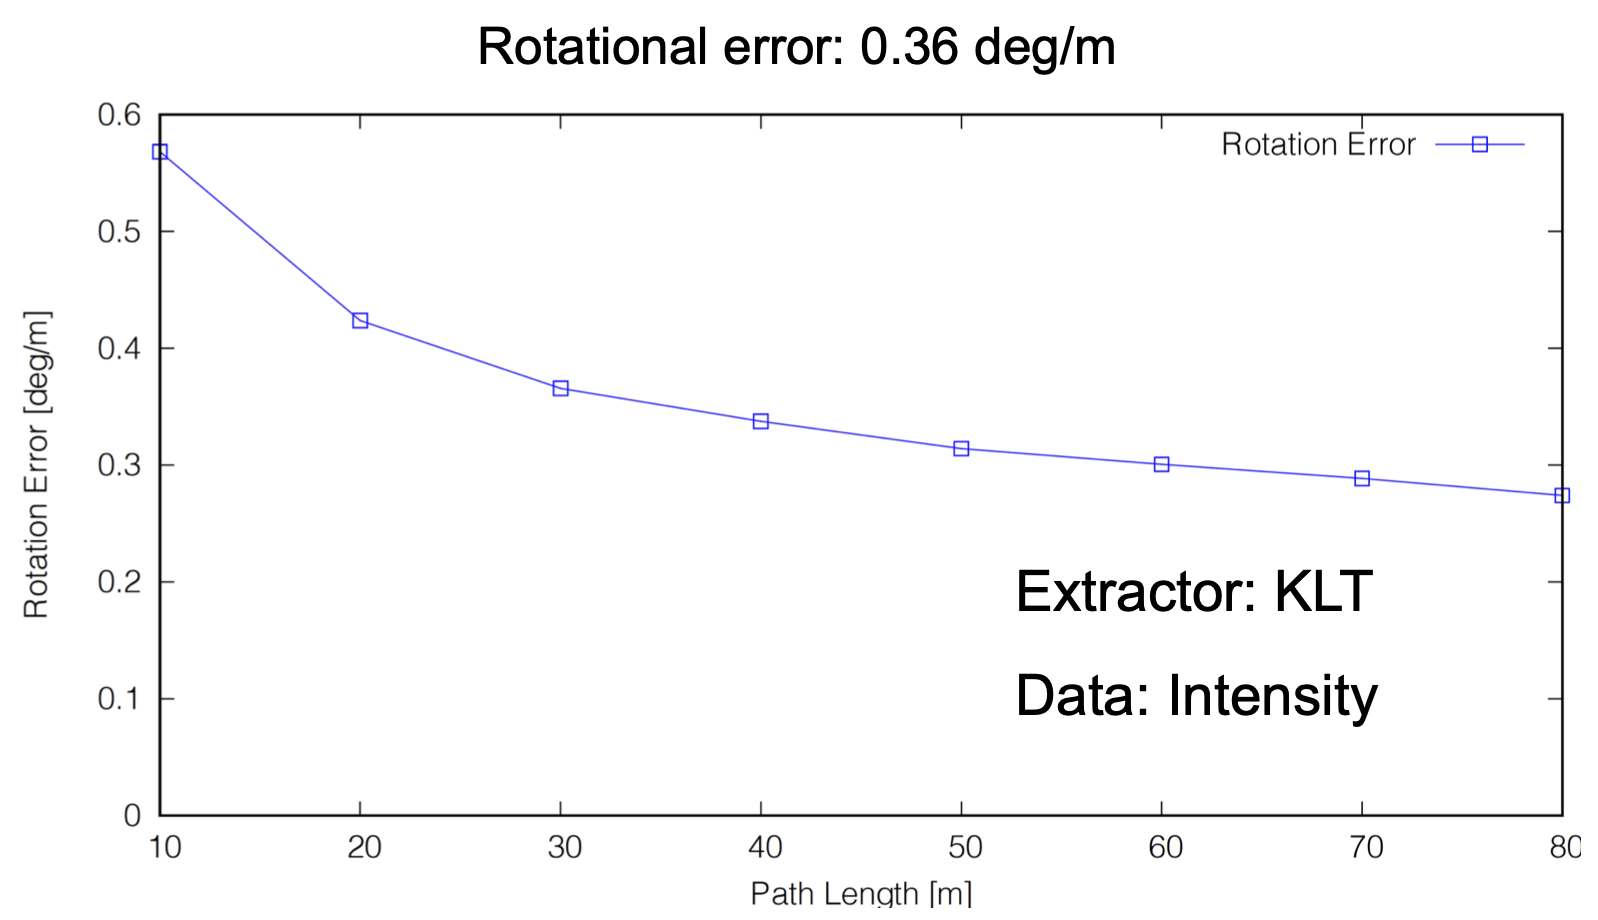
\includegraphics[scale = 0.45]{images/results/mm_drift_angle.png}
%                     \caption{KLT angular drift}
%                     \label{fig:KLT_drift_angle}
%                 \end{figure}
%             }
%             As we can see on the drift plots \cref{fig:ORB_drift_transl} to \cref{fig:KLT_drift_angle} ORB performs slightly better than KLT for the considered dataset.
                    
%         }
%         \clearpage
%         \subsection{Verdict Feature Methods}{

%             Starting of with the step comparison ORB and KLT indicate a slightly better performance than BRISK. 

%             With the additional consideration of BRISKs comparatively poor TP rate and higher computational cost I would chose ORB or KLT over BRISK for the endeavor pursued in this work.

%             Then for the comparison of ORB and KLT we can see that ORB performs a little bit better considering the global drift error. However we have to consider the fundamental difference in their procedure. While ORB is dependent on the extraction of points at each iteration KLT can make use of previously detected points. This can be an advantage especially in feature-scarce environments. This is shown well in the additinal performance results section \cref{sec:additional_results}. So for a final verdict in this comparison I would use ORB on feature rich environments while KLT is more consistent in repetitive and feature scarce surroundings.
%             \clearpage
%         }

        
%     }
    
% \section{Final Comparison of Complementary Data}{

%     \subsection{Local Step Comparison – projection types}{

%     \begin{tabular}{p{2cm} p{3.5cm} p{3.5cm} p{2cm}}
%         \textbf{Errors} & \textbf{Intensity} & \textbf{Ambient} & \textbf{Range}
%     \end{tabular}

%     \begin{table}[!ht]
%         \setlength{\extrarowheight}{5pt}
%         \centering
%         \large
%         \begin{tabular}{p{1.3cm}| p{1.5cm} p{1.5cm}| p{1.5cm} p{1.5cm}| p{1.5cm} p{1.5cm}}
%             \hline
%                 & Mean & STD & Mean & STD & Mean & STD\\[12pt]
%             \hline
%             X[m] & -0.004 & \text{\color{Cyan}{0.056}} & -0.007 & 0.060 & \text{\color{Green}{-0.002}} & 0.102\\[3pt]
%             \hline
%             Y[m] & \text{\color{Green}{0}} & \text{\color{Cyan}{0.040}} & -0.001 & 0.042 & -0.008 & 0.170\\[3pt]
%             \hline
%             Z[m] & -0.001 & \text{\color{Cyan}{0.058}} & \text{\color{Green}{0}} & 0.060 & \text{\color{Green}{0}} & 0.098\\[3pt]
%             \hline
%             Roll[°] & \text{\color{Green}{0}} & \text{\color{Cyan}{0.024}} & \text{\color{Green}{0}} & \text{\color{Cyan}{0.024}} & 0.001 & 0.072\\[3pt]
%             \hline
%             Pitch[°] & \text{\color{Green}{0}} & \text{\color{Cyan}{0.024}} & \text{\color{Green}{0}} & \text{\color{Cyan}{0.024}} & \text{\color{Green}{0}} & 0.039\\[3pt]
%             \hline
%             Yaw[°] & \text{\color{Green}{0}} & \text{\color{Cyan}{0.029}} & \text{\color{Green}{0}} & \text{\color{Cyan}{0.029}} & \text{\color{Green}{0}} & 0.040\\[3pt]
%         \end{tabular}
%         \caption{Average Step Error Comparison for Complementary Data}
%         \label{tab:step_errors_data}
%     \end{table}

%     In \cref{tab:step_errors_data} intensity performs best directly followed best by the ambient data. Range falls off considering the standard deviation.
%     }

    
    
%     \subsection{Trajectory Comparison – projection types}{

%         \begin{figure}[!ht]
%             \centering
%             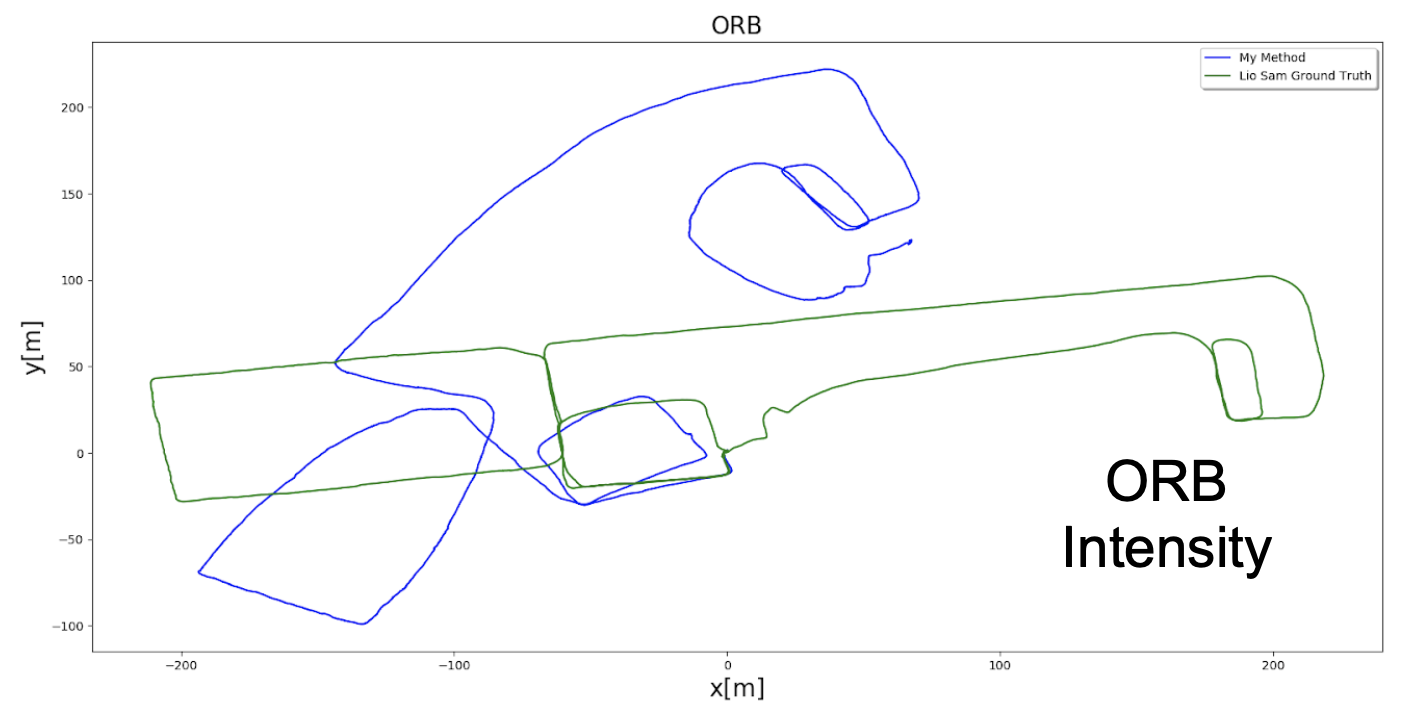
\includegraphics[scale = 0.5]{images/comparison_appendix/ORBt.png}
%             \caption{ORB trajectory}
%             \label{fig:ORB_trajectory_data}
%         \end{figure}
%         \clearpage

%         \begin{figure}[!ht]
%             \centering
%             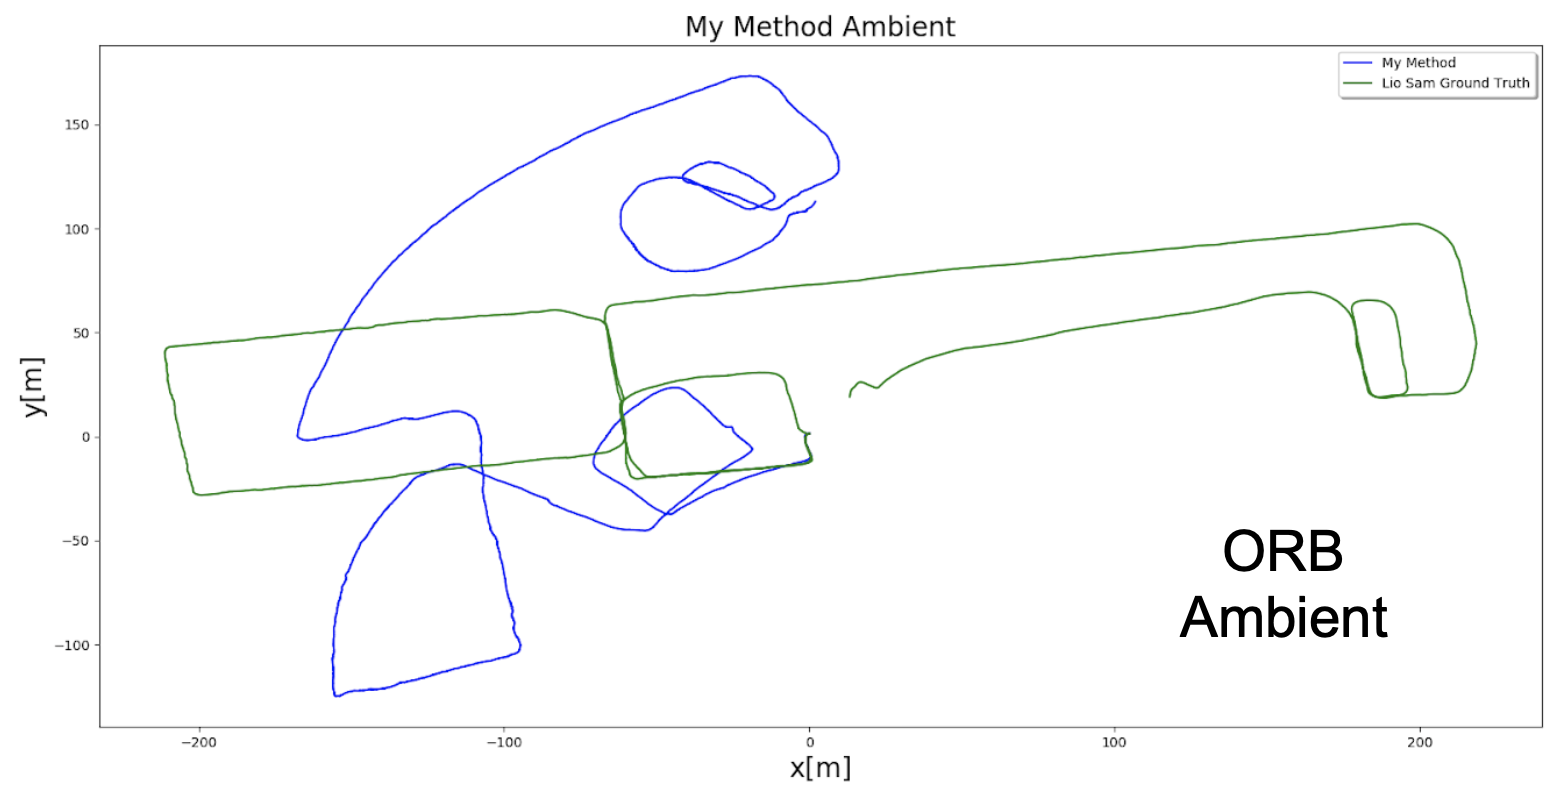
\includegraphics[scale = 0.5]{images/comparison_appendix/Ambientt.png}
%             \caption{Ambient trajectory}
%             \label{fig:ambient_trajectory}
%         \end{figure}

%         \begin{figure}[!ht]
%             \centering
%             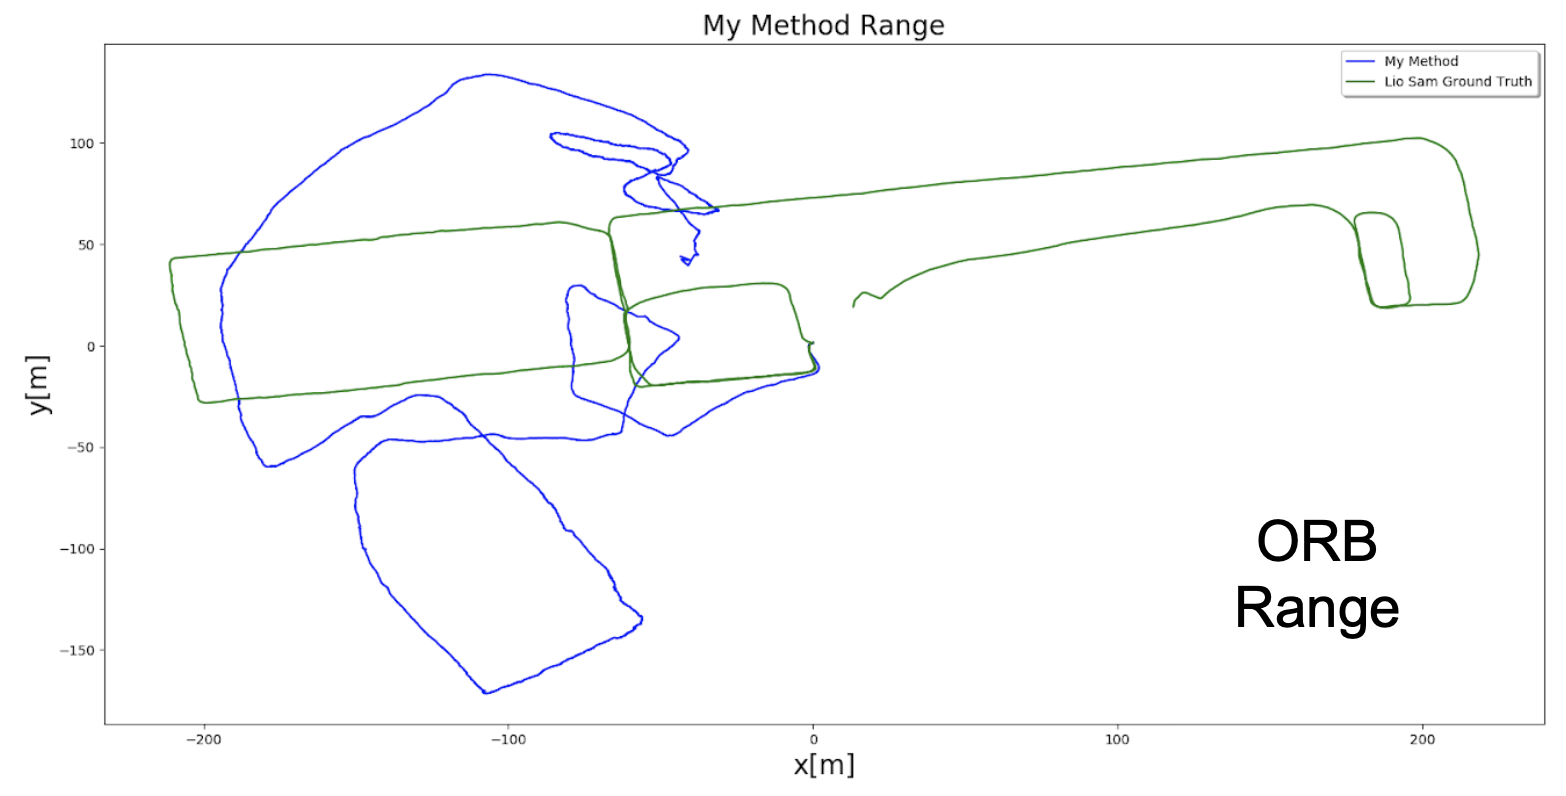
\includegraphics[scale = 0.5]{images/comparison_appendix/Ranget.png}
%             \caption{Range trajectory}
%             \label{fig:range_trajectory_method}
%         \end{figure}

%     }
%     \clearpage

%     \subsection{Drift Comparison – projection types}{
%         Analogously the accumulated drift comparison for the two more promising data types intensity and ambient:
%         \subsubsection{Translational Drift - projection types}{
%             \begin{figure}[!ht]
%                 \centering
%                 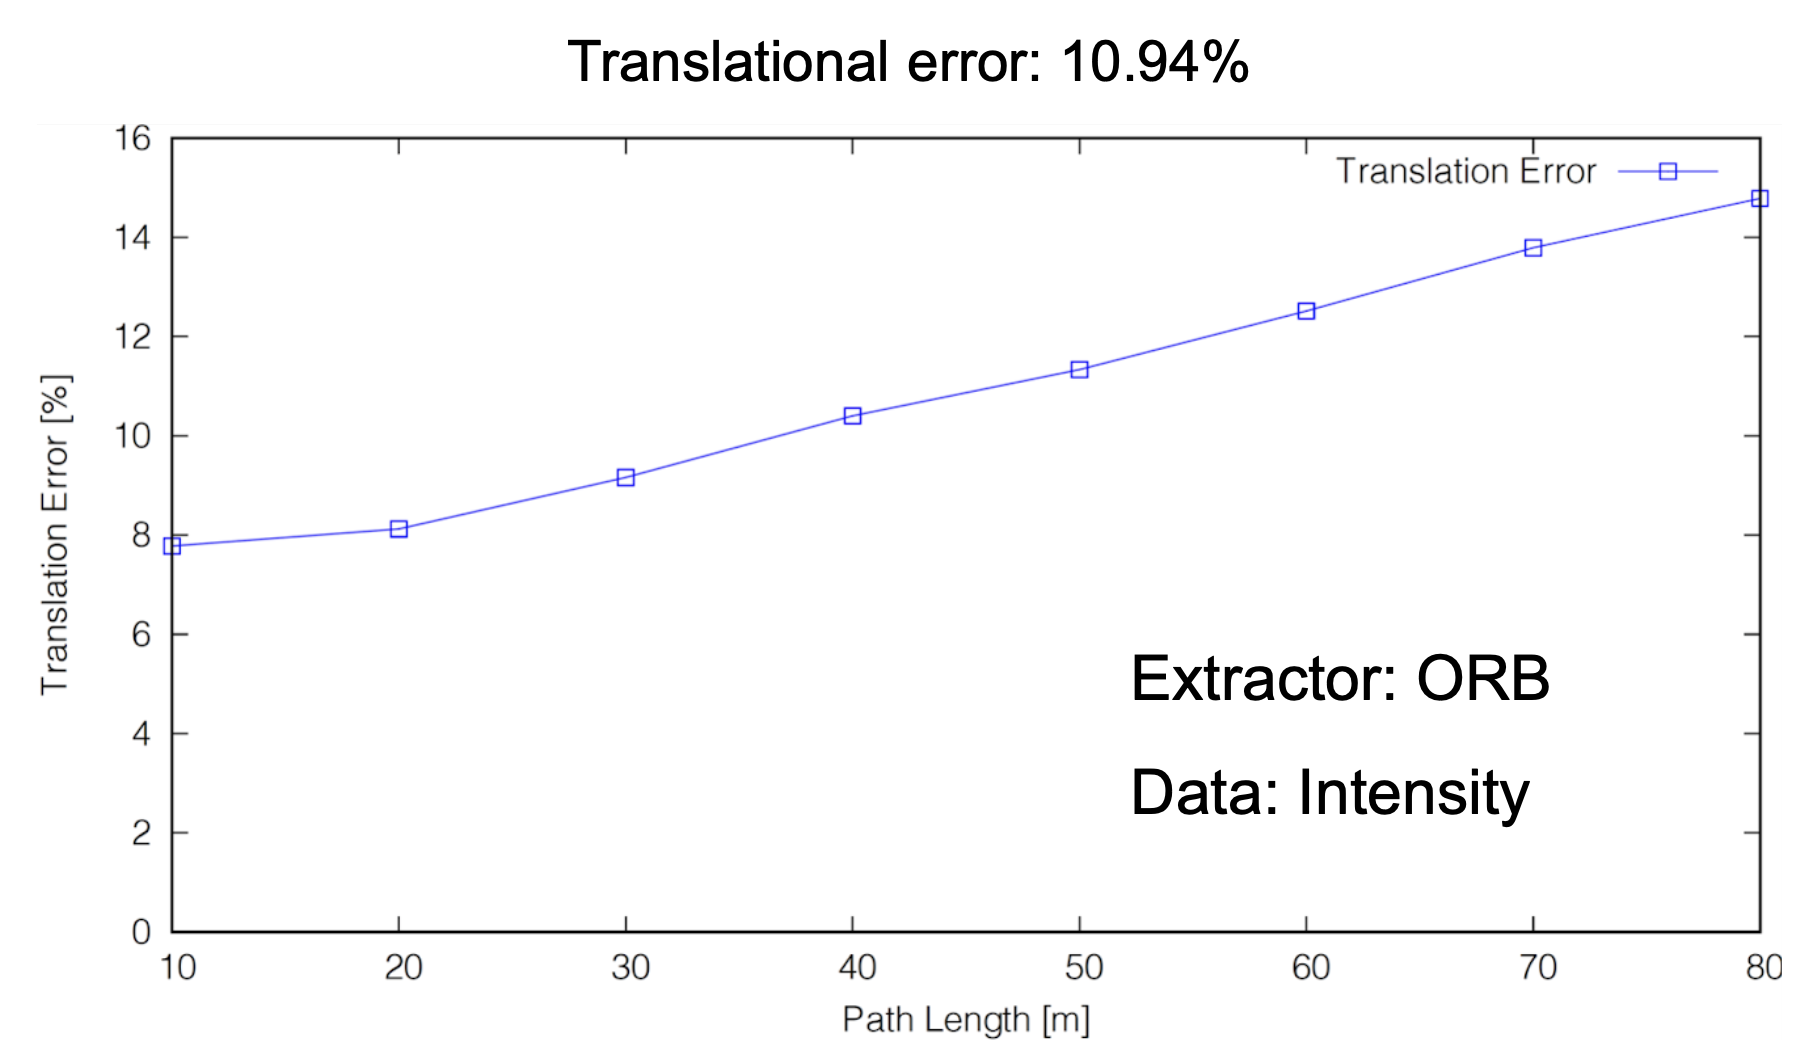
\includegraphics[scale = 0.4]{images/comparison_appendix/orb_drift_transl.png}
%                 \caption{Intensity drift translation}
%                 \label{fig:intensity_drift_transl}
%             \end{figure}

%             \begin{figure}[!ht]
%                 \centering
%                 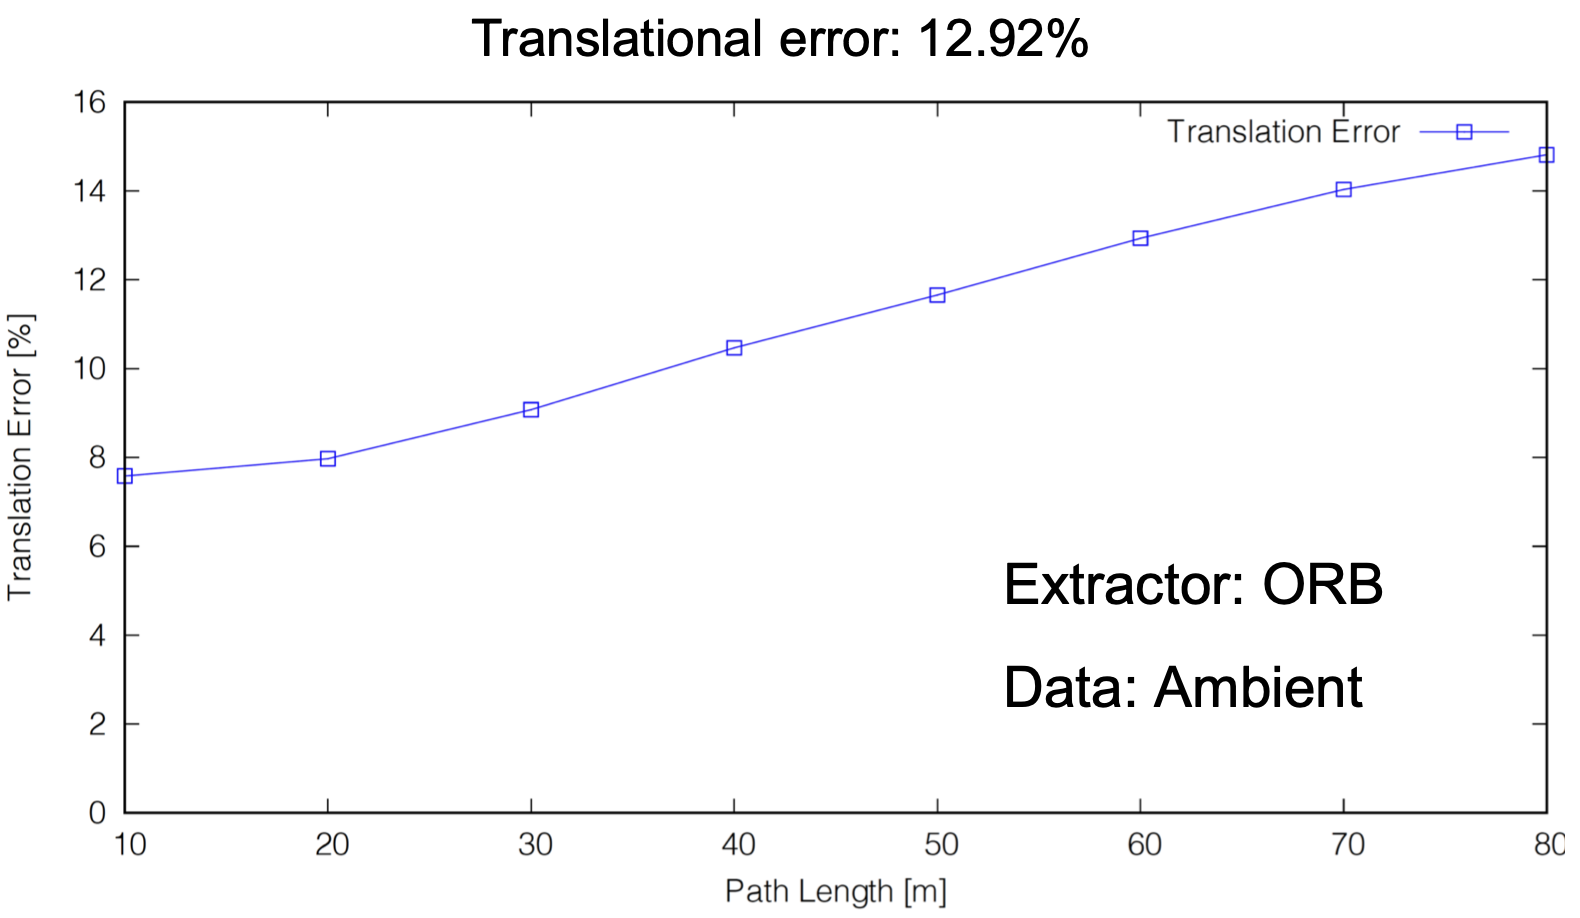
\includegraphics[scale = 0.45]{images/comparison_appendix/ambient_drift_translation.png}
%                 \caption{Ambient drift translation}
%                 \label{fig:ambient_drift_transl}
%             \end{figure}

%         }
%         \clearpage
%         \subsubsection{Angular Drift - projection types}{
%             \begin{figure}[!ht]
%                 \centering
%                 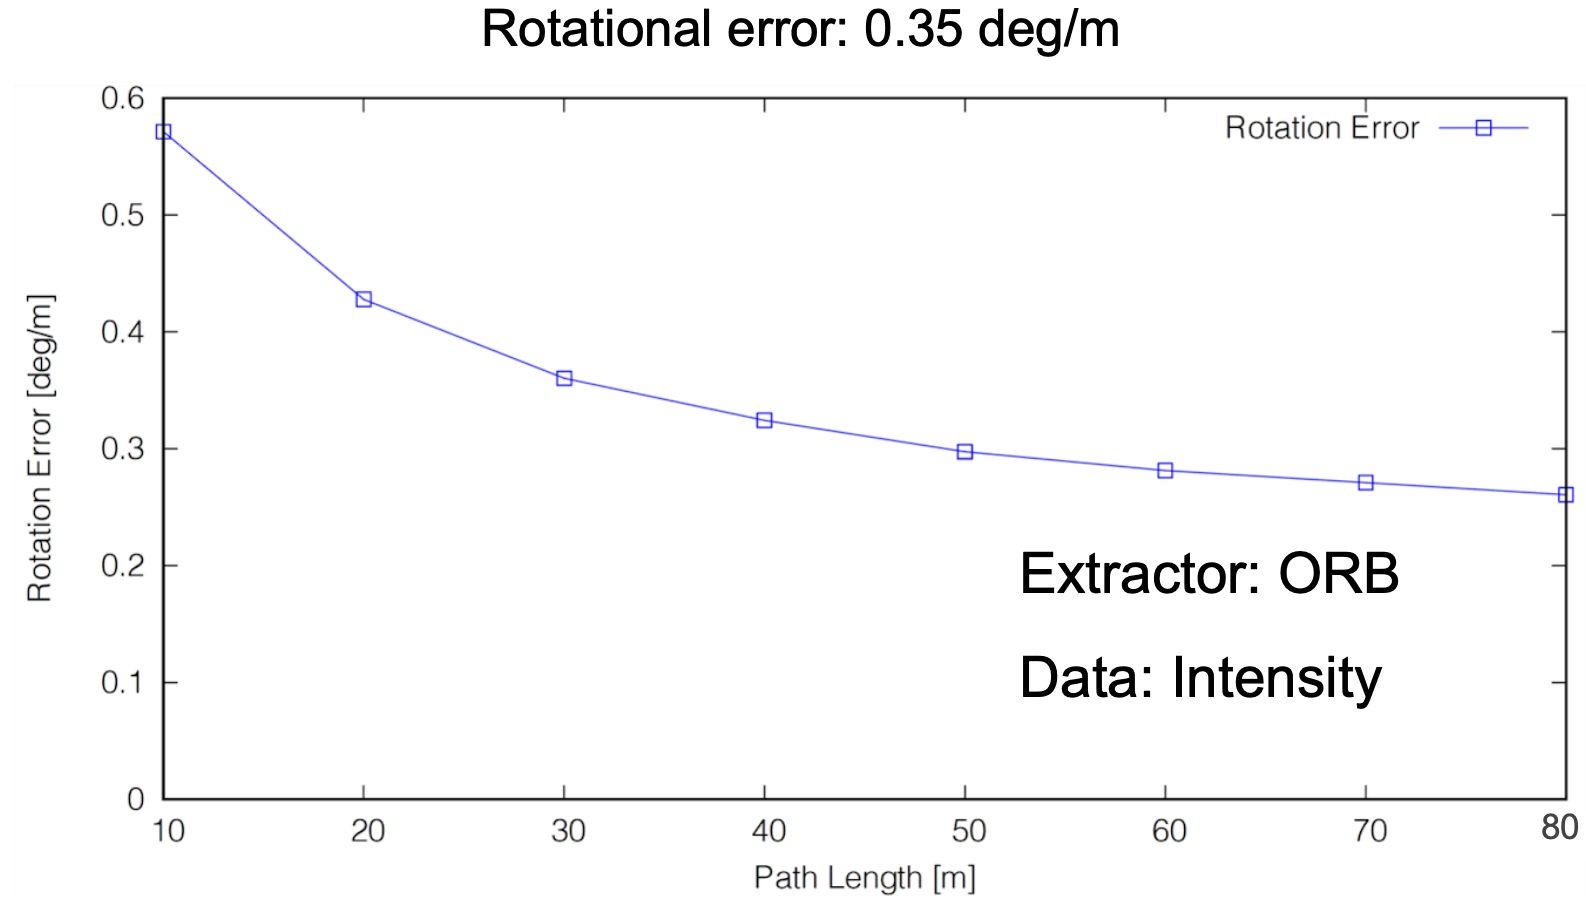
\includegraphics[scale = 0.43]{images/comparison_appendix/orb_drift_angle.png}
%                 \caption{Intensity angular drift}
%                 \label{fig:intensity_drift_angle}
%             \end{figure}

%             \begin{figure}[!ht]
%                 \centering
%                 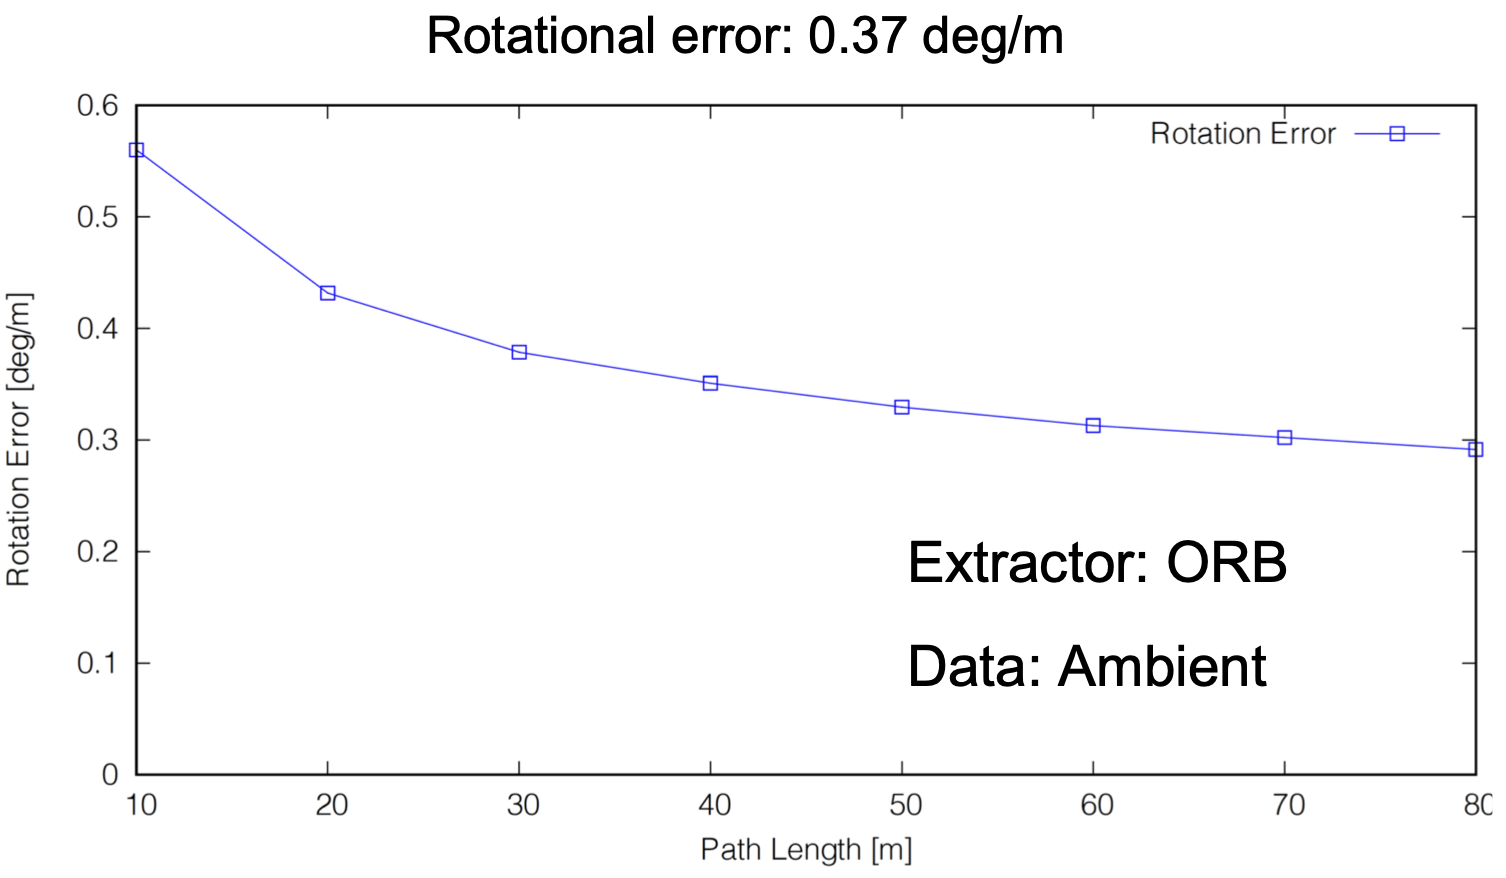
\includegraphics[scale = 0.45]{images/comparison_appendix/ambient_drift_angle.png}
%                 \caption{Ambient angular drift}
%                 \label{fig:ambient_drift_angle}
%             \end{figure}

%         }
%         On the drift plots \cref{fig:intensity_drift_transl} to \cref{fig:ambient_drift_angle} we see the intensity data performing better than ambient.
%     }
%     \clearpage
%     \subsection{Verdict Complementary Data}{

%     For this comparison the story is very similar for each stage in the progression. Intensity and ambient data perform equally well as the data source with a small advantage of intensity data. Range however falls off heavily. This can be seen throughout the whole pipeline. Fewer matches were built, a smaller TP rate was detected, bigger iterative as well as global errors could be found and a worse trajectory estimation resulted. 

%     \vspace{0.5cm}
%     The small gap between intensity and ambient data becomes noticeable when considering the laser intensities light independent nature. Therefore my choice for the optimal data source is intensity while keeping the ambient data in mind. Of course a combination of the data sources (and feature methods) considered would be a better solution still but this work revolved exclusively around individual performance comparison.
%     }

% }
% \clearpage

% \section{Additional Performance Results}\label{sec:additional_results}{
%     \subsection{Map Construction using found Transformation}{
%         With the pose estimation and the iterative scans we can build a map as depicted in \cref{fig:local_mapping} and \cref{fig:global_mapping}.
%         \begin{figure}[ht]
%             \centering
%             \includegraphics[scale=0.15]{images/appendix_additionals/map_before.png}
%             \caption{Local mapping performance}
%             \label{fig:local_mapping}
%         \end{figure}
        
%         \begin{figure}[ht]
%             \centering
%             \includegraphics[scale=0.15]{images/appendix_additionals/map_after.png}
%             \caption{Mapping drift after walking one block}
%             \label{fig:global_mapping}
%         \end{figure}

%         As we can see in \cref{fig:local_mapping} locally the estimation is really accurate leading to a detailed map of the surroundings.

%         After having gone around the building block in the dataset however the mapping process shows accumulated drift. (\cref{fig:global_mapping})

%         For a perfect transformation the red-white arrows should be aligned and should lead back to the start position indicated with the black circle.

%     }
%     \clearpage

%     \subsection{Alternative Dataset 1: Indoor}{
%         For a first alternative to the outside dataset I considered an indoor scan from the same paper\citep{robust2021shan} as the handheld dataset. In this dataset three laps are walked through an office space with small corridors. Before the third lap however the LiDAR sensor is turned upside down.

%         \begin{figure}[ht]
%             \centering
%             \includegraphics[scale=0.25]{images/appendix_additionals/indoor_klt.png}
%             \caption{Indoor Dataset using KLT}
%             \label{fig:indoor_klt}
%         \end{figure}

%         As we can see there is certain drift accumulating but only slowly. Locally the performance seems quite robust. Also interestingly there is no observable decrease in performance after the second loop. (Sensor turning point)
        
%         This result was achieved using the KLT method. So far ORB and KLT had performed similarly with ORB having slightly smaller errors. Here for this dataset however we have to work with very little features and repetitive surroundings in the corridors. The impact of this can be seen in \cref{fig:indoor_orb} when using ORB:
        
%         \begin{figure}[ht]
%             \centering
%             \includegraphics[scale=0.25]{images/appendix_additionals/indoor_orb.png}
%             \caption{Indoor Dataset using ORB}
%             \label{fig:indoor_orb}
%         \end{figure}

%         As we can see ORB performs significantly worse than KLT starting at the entrance point of the corridor (indicated with the white circle) this is of course due to the lack of detectable features while KLT can make use of previously detected key points.

%     }
%     \clearpage

%     \subsection{Alternative Dataset 2: Excavator}{
%     As a second alternative dataset I considered the excavator dataset from the rsl lab.

%     \begin{figure}[ht]
%         \centering
%         \includegraphics[scale=0.15]{images/appendix_additionals/excavator.png}
%         \caption{Map construction on excavator dataset}
%         \label{fig:excavator_map}
%     \end{figure}

%     \normalsize
%     As the name lets assume this dataset is from the point of view of an excavator on a very vast landscape with few features that are located far away. In the lower half of this \cref{fig:excavator_map} we see the map building process analogously to \cref{fig:local_mapping}. Here we see poor performance due to the lack of features and the big distances to them.
% }
% }

% \clearpage
% \chapter{Conclusion}\label{sec:conclusion}

The initial problem setting in this project was to pave the way for the creation of an AR handheld remote control for an autonomous excavator. The following two requirements were tackled:

\section{Data Transfer}\label{sec:conc_data_transfer}
The proposed method in this work was to use an Unreal Engine multiplayer connection for the information sharing process. This seems to be a working solution with a few persisting obstacles which have to be worked around before implementing it in the pipeline. 

\subsection{Checksum Inequality}\label{subsec:checksum_error}

When the colocalization requirement is tackled using the Azure Spatial Anchor approach as described in \cref{ch:colocalization} then the problem of unequal checksums arises. This has to be worked around. Currently the following options come to mind:
\begin{itemize}
    \item Sequentially changing the handheld game structure in order to reach the desired initial checksum again. (Due to limited documentation of the checksum generation this is mostly educated guesswork)
    \item Finding a way of manually overriding the generated checksum in the handheld UE instance
    \item Making use of a different subsystem as for instance Steam\footnote{Steam Online Subsystem\\ \url{https://docs.unrealengine.com/4.27/en-US/ProgrammingAndScripting/Online/Steam/}} provides. This option provides a robust solution with the drawback that one more piece of software is necessary on the excavator which naturally is undesirable.
\end{itemize}

\subsection{Unreliable Local Connection}\label{subsec:unrealiable_connection}

Throughout this project many different network settings were tested and even with sufficient network speed the multiplayer connection between the UE instances was not reliable. To draw a definite conclusion here more tests would be necessary however a possibility might be to use a dedicated server\footnote{as described in \cref{sec:multiplayer}} on the excavator instead of the client - server model.

\section{Colocalization}\label{sec:conc_colocalization}

The Azure Spatial Anchor set up allows for quite an easy implementation as the colocalization process is handled completely by this module given the successful creation and detection of such a spatial anchor.

As seen in \cref{sec:colocalization_testing} the anchor creation tends to have a shift in its location. Apart from this the colocalization pipeline seems very reliable with robustness regarding both ambient changes as well as repeatability. As it is not apparent where this shift of the anchor location is introduced it would be best to perform tests with the actual excavator setup directly. 

\section{Outlook}\label{sec:outlook}

 With the state transfer connection working between the two UE instances any other piece of data can be converted into an Unreal Engine game component and shared in the same way. A more robust connection between the devices would be beneficial however.
 
 This very same connection can be used to give orders from the handheld device to the excavator given that the UE connection remains a client-server relationship.

As the inclusion of the Azure Spatial Anchor plugin renders the connection unviable for the time being this has to be looked into further as indicated in \cref{sec:conc_data_transfer}. Alternatively a different method for colocalization would be necessary. 

So all in all this project provides two individual modules that solve the two respective key requirements of handheld remote control for autonomous excavators. However for now there are still complications prohibiting this joint setup.


% \clearpage

\chapter{Introduction}
\label{ch:introduction}


When operating an excavator in the conventional fashion two requirements are imperative: \begin{itemize}
    \item The view onto the construction site
    \item The handles necessary to give inputs to the machine
\end{itemize}
In the case of an autonomous excavator the low level actions to perform are determined by the machine itself, given a high level action input. So in this case the second requirement becomes the possibility to give such a high level input to the system.

With the desired handheld remote control setup the necessity of sharing information between the device and the machine still persists. The visual requirements change however. From the handheld camera we now receive the required view of the surroundings on the construction site but in order to successfully share a geometric location with the excavator the colocalization problem has to be solved for the two players. Having an AR remote control integrated in a handheld device also provides the possibility of introducing further useful features such as displaying a preview of an action of choice. 

In this project I attempted to overcome the key challenges constituting the requirements mentioned above. 

The plan was to solve the data transfer requirement utilizing the already implemented Unreal Engine setup of the autonomous excavator\footnote{HEAP - The autonomous walking excavator\citep*{heap}} from the Robotic Systems Laboratory. To account for the colocalization problem an approach using Microsoft's Azure Spatial Anchors was used.
\clearpage
\chapter{Related Work}\label{ch:related_work}

% The work related to this thesis can be divided into two categories:

% First there is the traditional 2D computer vision aspect to it for which I can't reference a specific work as the field is just too broad. However some crucial mentions are the different feature methods that I considered in this work (ORB\footnote{Oriented FAST and Rotated BRIEF \citep{ORB}}, BRISK \footnote{BRISK: Binary Robust Invariant Scalable Keypoints \citep{BRISK}} and KLT\footnote{Lucas Kanade Tracking \citep{KLT}}) as well as the outlier rejection procedure RANSAC\footnote{RANdom SAmple Consensus\citep{ransac}}.

% The second part concerns the 3D side of the paper being state of the art LiDAR usage for motion estimation:

% LiDAR as a tool is of course no new idea and many ingenious people have already 
% ventured into this field and refined methods to work with the 3D data that LiDAR 
% provides us with. The traditional procedure for achieving motion estimation using LiDAR is point cloud registration and there have been a lot of papers published about this idea. One that I would like to point out is the paper of Pomerleau et al. \footnote{A Review of Point Cloud Registration Algorithms for Mobile Robotics \citep{Pomerleau}} which summarizes the ICP algorithm (Iterative Closest Point) as well as certain usage cases.

% An alternative procedure to estimate the motion and construct a map of the surroundings at run time is LOAM \footnote{LiDAR Odometry and Mapping \citep{LOAM}} which is built around the idea of splitting the two algorithms up into the odometry and the mapping part.
% For the odometry part the detected features are divided into planar patches and sharp edge lines which are then used to establish correspondences and thus achieve motion estimation. 
% The mapping process makes use of the iterative scans as well as the transformations each step in order to build the permanent map in the world frame. This map in turn can be consulted in order to achieve much more accurate motion estimation.\\

% This bachelor thesis however was built on the idea of projecting dense point clouds of newer LiDAR scans onto planes and performing state of the art 2D CV methods on the projections as opposed to applying computationally expensive alignment methods. I thus used the best of both worlds by achieving run time performance without neglecting a significant amount of information through downsampling the point clouds. 
% \clearpage
% With great probability the first paper published about this new way of working with LiDAR data is the paper of Shan et al. \footnote{Robust place recognition using an imaging lidar \citep{robust2021shan}} In their work they used this approach in order to extract ORB features each scan and to build up a BoW database which they queried in order to find matches with later extracted features to determine loop closures. In comparison to their work I used this underlying method in order to achieve motion estimation considering just two subsequent scans as well as different descriptors and complementary types of data.

Certainly the most important related work and the reason this project can even take place is the autonomous excavator heap\citep*{heap} itself. 

Overall the methods chosen in this project are very applied and unconventional which is why there is little related work to be cited. It has to be mentioned however that the whole structure of Unreal Engine multiplayer connections has to be considered for this project. Especially cross platform multiplayer connections were essential for this work. Secondly the Azure Spatial Anchors process is also a fundamental building stone for the procedure used here.
\clearpage
\chapter{Method}\label{ch:method}

As mentioned above the approach in this project can be divided into two stages:

\begin{figure}[ht]
    \centering
    \includegraphics[scale = 0.32]{images/method/method.png}
    \caption{High level handheld remote setup}
    \label{fig:method}
\end{figure}

\begin{itemize}
    \item Data transfer between the excavator and the handheld device (left arrow connection)
    \begin{itemize}
        \item Creating an Augmented Reality Unreal Engine (UE) game on the handheld device
        \item Making use of the already existing UE interface on the excavator to store system information in game components 
        \item Using an Unreal Engine local multiplayer connection in order to transfer data between the two UE instances
    \end{itemize}
    \item Colocalization between the two frames of reference (right arrow connection) 
    \begin{itemize}
        \item Extracting a spatial anchor from the excavator's camera view using a ROS wrapper 
        \item Uploading this visual anchor in the form of an Azure Spatial Anchor to the Azure cloud
        \item Retrieving the stored spatial anchor in the handheld UE instance 
        \item Using the spatial anchor to relocate the UE world origin
    \end{itemize}
\end{itemize}





\clearpage
% \chapter{Results}\label{sec:results}

% \section{Ground Truth}{
    
%     As there wasn't a GT for my dataset I considered the very accurate and map based Lio-Sam\footnote{LIO-SAM: Tightly-coupled Lidar Inertial Odometry via Smoothing and Mapping \citep{liosam2020shan}} estimation as the GT for this work. 
    
%     I also considered LOAM\footnote{LiDAR Odometry And Mapping \citep{LOAM}} for another comparison and very importantly as a third and most meaningful alternative I chose the LOAM method without the map procedure as well. This is because my approach is scan based and does not build a map which of course enhances accuracy significantly. So comparing to a scan based method is the only fair comparison.


%     }

% \section{Stepwise Results}{

%     \subsection{Comparison of Separated Components}{
%     \begin{figure}[ht]
%         \centering
%         \includegraphics[scale = 0.26]{images/results/steps_klt.png}
%         \caption{Step comparison}
%         \label{fig:step_comparison_klt}
%     \end{figure}

%     In \cref{fig:step_comparison_klt} we can see the step comparison of the three directions as well as the rotation angles. 
    
%     We can also consider the errors at each iteration depicted in the following \cref{fig:step_error_comparison_klt}
%     \begin{figure}[ht]
%         \centering
%         \includegraphics[scale = 0.285]{images/results/step_error_klt.png}
%         \caption{Step Error comparison}
%         \label{fig:step_error_comparison_klt}
%     \end{figure}



%     As we can see in the figures \cref{fig:step_comparison_klt} and \cref{fig:step_error_comparison_klt} there are outliers in the method. However both the step error of this papers method as well as the iterative error of the scan based LOAM method yield values in the same range.

%     }

%     \subsection{Average Step Performance Comparison}{
%     Mean iterative error and standard deviation thereof regarding GT over the whole dataset:

%         \vspace{0.5cm}
        
%         \large
%         \begin{tabular}{p{3cm} p{4.5cm} p{3.5cm} }
%             \textbf{Errors} & \textbf{My Method} & \textbf{LOAM S2S}
%         \end{tabular}

%         \begin{table}[!ht]
%             \setlength{\extrarowheight}{5pt}
%             \centering
%             \large
%             \begin{tabular}{p{2cm} p{2cm} p{2cm} p{2cm} p{2cm} }
%                 \hline
%                  & Mean & STD & Mean & STD\\[12pt]
%                 \hline
%                 X[m] & -0.004 & 0.056 & \text{\color{Green}{-0.002}} & \text{\color{Cyan}{0.035}}\\[3pt]
%                 \hline
%                 Y[m] & \text{\color{Green}{0}} & 0.040 & 0.005 & \text{\color{Cyan}{0.028}}\\[3pt]
%                 \hline
%                 Z[m] & \text{\color{Green}{-0.001}} & 0.058 & -0.004 & \text{\color{Cyan}{0.032}}\\[3pt]
%                 \hline
%                 Roll[°] & \text{\color{Green}{0}} & 0.024 & \text{\color{Green}{0}} & \text{\color{Cyan}{0.021}}\\[3pt]
%                 \hline
%                 Pitch[°] & \text{\color{Green}{0}} & 0.024 & -0.001 & \text{\color{Cyan}{0.020}}\\[3pt]
%                 \hline
%                 Yaw[°] & \text{\color{Green}{0}} & 0.024 & \text{\color{Green}{0}} & \text{\color{Cyan}{0.023}}\\[3pt]
%             \end{tabular}
%             \caption{Average Step Error Comparison}
%             \label{tab:step_errors_klt}
%         \end{table}

%         The data displayed in \cref{tab:step_errors_klt} was achieved using the KLT method on intensity data. Green values are the best achieved mean while light blue indicates the best standard deviation.   

%         When evaluating the numbers we see for my method smaller mean errors on average while LOAM scan 2 scan has smaller deviations from the slightly larger mean error.

        
%     }

% \section{Global Results}{
%     \subsection{Comparison of Separated Components}{

%     Comparing the individual pose components:

%         \begin{figure}[ht]
%             \centering
%             \includegraphics[scale = 0.25]{images/results/pose_klt.png}
%             \caption{Pose comparison}
%             \label{fig:pose_comparison_klt}
%         \end{figure}

%         \begin{figure}[ht]
%             \centering
%             \includegraphics[scale = 0.25]{images/results/pose_error_klt.png}
%             \caption{Pose error comparison}
%             \label{fig:pose_error_comparison_klt}
%         \end{figure}

%         Here in \cref{fig:pose_comparison_klt} and \cref{fig:pose_error_comparison_klt} we can see substantially better global performance of this works method especially regarding the angular development.

%     }

%     \subsection{Comparison of Global Error}{
%         \begin{figure}[ht]
%             \centering
%             \includegraphics[scale = 0.45]{images/results/mm_drift_translation.png}
%             \caption{My methods translational drift}
%             \label{fig:mm_drift_transl_klt}
%         \end{figure}
        
%         \begin{figure}[ht]
%             \centering
%             \includegraphics[scale = 0.4]{images/results/loam_drift_transl.png}
%             \caption{LOAM translational drift}
%             \label{fig:loam_drift_transl_klt}
%         \end{figure}
        
%         To account for the drift of the motion estimation a comparison was done after predetermined distance intervals. Here in \cref{fig:mm_drift_transl_klt} to \cref{fig:loam_drift_transl_klt} are the values for the intervals from 10 to 80 meters. It has to be noted that 80 meters is quite a distance and the results from that margin onwards might be slightly deceiving compared to more solid smaller intervals. 
        
%         Averaged over all interval sizes my methods performs a little better as can be seen from the averaged translational error denoted at the top.

%         \clearpage

%         \begin{figure}[ht]
%             \centering
%             \includegraphics[scale = 0.45]{images/results/mm_drift_angle.png}
%             \caption{My methods angular drift}
%             \label{fig:mm_drift_angle_klt}
%         \end{figure}

%         \begin{figure}[!ht]
%             \centering
%             \includegraphics[scale = 0.4]{images/results/loam_drift_angle.png}
%             \caption{loam angular drift}
%             \label{fig:loam_drift_angle_klt}
%         \end{figure}

%         A similar result can be drawn from the angular development. This papers method shows with 0.35 degrees/meter a better performance than the LOAM scan to scan method.
%     }
%     \clearpage

%     \subsection{Comparing Estimated Trajectories}{
%         \begin{figure}[!ht]
%             \centering
%             \includegraphics[scale = 0.45]{images/results/GT_trajectory.png}
%             \caption{GT trajectory}
%             \label{fig:GT_trajectory}
%         \end{figure}

%         Indicated on the plot above is the datasets trajectory estimated by Lio-Sam. This will again be considered the ground truth.

%         \begin{figure}[!ht]
%             \centering
%             \includegraphics[scale = 0.45]{images/results/loam_s2m_trajectory.png}
%             \caption{LOAM scan to map trajectory}
%             \label{fig:loam_s2m_trajectory}
%         \end{figure}

%         As aforementioned the LOAM method performs very well as it is also map based and thus really accurate.
%         \clearpage

%         \begin{figure}[!ht]
%             \centering
%             \includegraphics[scale = 0.45]{images/results/loam_s2s_trajectory.png}
%             \caption{LOAM scan to scan trajectory}
%             \label{fig:loam_s2s_trajectory}
%         \end{figure}

%         Considering the solely scan based LOAM estimation it looks quite poor.

%         \begin{figure}[!ht]
%             \centering
%             \includegraphics[scale = 0.45]{images/results/mm_trajectory.png}
%             \caption{This works methods trajectory}
%             \label{fig:mm_trajectory}
%         \end{figure}

%         When looking at method from this paper it does accumulate quite some drift but performs considerably better than the scan based LOAM implementation. For additional performance results of this method consult \cref{sec:additional_results}
%     }
%     \clearpage
% }

    
% \section{Final Comparison of Feature Methods}{
%         In this section I will perform a comparison of the feature methods to the point of a possible verdict. For in depth data about each respective method consult \cref{ch:additional_plots}

%         \subsection{Local Step Comparison – feature methods}{

%         \begin{tabular}{p{2cm} p{3.5cm} p{3.7cm} p{2cm}}
%             & \textbf{ORB} & \textbf{BRISK} & \textbf{KLT}
%         \end{tabular}

%         \begin{table}[!ht]
%             \setlength{\extrarowheight}{5pt}
%             \centering
%             \large
%             \begin{tabular}{p{1.3cm}| p{1.5cm} p{1.5cm}| p{1.5cm} p{1.5cm}| p{1.5cm} p{1.5cm}}
%                 \hline
%                 \textbf{Errors} & Mean & STD & Mean & STD & Mean & STD\\[12pt]
%                 \hline
%                 X[m] & -0.004 & 0.056 & 0.004 & 0.219 & \text{\color{Green}{-0.003}} & \text{\color{Cyan}{0.048}}\\[3pt]
%                 \hline
%                 Y[m] & \text{\color{Green}{0}} & 0.040 & \text{\color{Green}{0}} & 0.117 & 0.001 & \text{\color{Cyan}{0.035}}\\[3pt]
%                 \hline
%                 Z[m] & -0.001 & 0.058 & -0.001 & 0.097 & \text{\color{Green}{0}} & \text{\color{Cyan}{0.046}}\\[3pt]
%                 \hline
%                 Roll[°] & \text{\color{Green}{0}} & \text{\color{Cyan}{0.024}} & 0.001 & 0.049 & \text{\color{Green}{0}} & 0.025\\[3pt]
%                 \hline
%                 Pitch[°] & \text{\color{Green}{0}} & \text{\color{Cyan}{0.024}} & \text{\color{Green}{0}} & 0.028 & \text{\color{Green}{0}} & \text{\color{Cyan}{0.024}}\\[3pt]
%                 \hline
%                 Yaw[°] & \text{\color{Green}{0}} & \text{\color{Cyan}{0.024}} & \text{\color{Green}{0}} & 0.048 & \text{\color{Green}{0}} & 0.029\\[3pt]
%             \end{tabular}
%             \caption{Average Step Error Comparison for Feature Methods}
%             \label{tab:step_errors_methods}
%         \end{table}

%         In \cref{tab:step_errors_methods} we can see the iterative performance of the feature methods. 
        
%         ORB and KLT seem to perform similarly while BRISK falls off a little regarding the standard deviation.

%         }
%         \subsection{Trajectory Comparison – feature methods}{

%         \begin{figure}[!ht]
%             \centering
%             \includegraphics[scale = 0.5]{images/comparison_appendix/ORBt.png}
%             \caption{ORB trajectory}
%             \label{fig:ORB_trajectory}
%         \end{figure}
%         \clearpage

%         \begin{figure}[!ht]
%             \centering
%             \includegraphics[scale = 0.5]{images/comparison_appendix/BRISKt.png}
%             \caption{BRISK trajectory}
%             \label{fig:BRISK_trajectory}
%         \end{figure}

%         \begin{figure}[!ht]
%             \centering
%             \includegraphics[scale = 0.5]{images/comparison_appendix/KLTt.png}
%             \caption{KLT trajectory}
%             \label{fig:KLT_trajectory_method}
%         \end{figure}
%         }
%         \clearpage
%         \subsection{Drift Comparison – feature methods}{
%             I also compared the more promising methods ORB and KLT regarding the accumulated drift:
%             \subsubsection{Translational Drift - feature methods}{
%                 \begin{figure}[!ht]
%                     \centering
%                     \includegraphics[scale = 0.4]{images/comparison_appendix/orb_drift_transl.png}
%                     \caption{ORB drift translation}
%                     \label{fig:ORB_drift_transl}
%                 \end{figure}

%                 \begin{figure}[!ht]
%                     \centering
%                     \includegraphics[scale = 0.45]{images/results/mm_drift_translation.png}
%                     \caption{KLT translational drift}
%                     \label{fig:KLT_drift_transl}
%                 \end{figure}
%                     }
%                 \clearpage
%             \subsubsection{Angular Drift - feature methods}{

%                 \begin{figure}[!ht]
%                     \centering
%                     \includegraphics[scale = 0.45]{images/comparison_appendix/orb_drift_angle.png}
%                     \caption{ORB angular drift}
%                     \label{fig:ORB_drift_angle}
%                 \end{figure}

%                 \begin{figure}[!ht]
%                     \centering
%                     \includegraphics[scale = 0.45]{images/results/mm_drift_angle.png}
%                     \caption{KLT angular drift}
%                     \label{fig:KLT_drift_angle}
%                 \end{figure}
%             }
%             As we can see on the drift plots \cref{fig:ORB_drift_transl} to \cref{fig:KLT_drift_angle} ORB performs slightly better than KLT for the considered dataset.
                    
%         }
%         \clearpage
%         \subsection{Verdict Feature Methods}{

%             Starting of with the step comparison ORB and KLT indicate a slightly better performance than BRISK. 

%             With the additional consideration of BRISKs comparatively poor TP rate and higher computational cost I would chose ORB or KLT over BRISK for the endeavor pursued in this work.

%             Then for the comparison of ORB and KLT we can see that ORB performs a little bit better considering the global drift error. However we have to consider the fundamental difference in their procedure. While ORB is dependent on the extraction of points at each iteration KLT can make use of previously detected points. This can be an advantage especially in feature-scarce environments. This is shown well in the additinal performance results section \cref{sec:additional_results}. So for a final verdict in this comparison I would use ORB on feature rich environments while KLT is more consistent in repetitive and feature scarce surroundings.
%             \clearpage
%         }

        
%     }
    
% \section{Final Comparison of Complementary Data}{

%     \subsection{Local Step Comparison – projection types}{

%     \begin{tabular}{p{2cm} p{3.5cm} p{3.5cm} p{2cm}}
%         \textbf{Errors} & \textbf{Intensity} & \textbf{Ambient} & \textbf{Range}
%     \end{tabular}

%     \begin{table}[!ht]
%         \setlength{\extrarowheight}{5pt}
%         \centering
%         \large
%         \begin{tabular}{p{1.3cm}| p{1.5cm} p{1.5cm}| p{1.5cm} p{1.5cm}| p{1.5cm} p{1.5cm}}
%             \hline
%                 & Mean & STD & Mean & STD & Mean & STD\\[12pt]
%             \hline
%             X[m] & -0.004 & \text{\color{Cyan}{0.056}} & -0.007 & 0.060 & \text{\color{Green}{-0.002}} & 0.102\\[3pt]
%             \hline
%             Y[m] & \text{\color{Green}{0}} & \text{\color{Cyan}{0.040}} & -0.001 & 0.042 & -0.008 & 0.170\\[3pt]
%             \hline
%             Z[m] & -0.001 & \text{\color{Cyan}{0.058}} & \text{\color{Green}{0}} & 0.060 & \text{\color{Green}{0}} & 0.098\\[3pt]
%             \hline
%             Roll[°] & \text{\color{Green}{0}} & \text{\color{Cyan}{0.024}} & \text{\color{Green}{0}} & \text{\color{Cyan}{0.024}} & 0.001 & 0.072\\[3pt]
%             \hline
%             Pitch[°] & \text{\color{Green}{0}} & \text{\color{Cyan}{0.024}} & \text{\color{Green}{0}} & \text{\color{Cyan}{0.024}} & \text{\color{Green}{0}} & 0.039\\[3pt]
%             \hline
%             Yaw[°] & \text{\color{Green}{0}} & \text{\color{Cyan}{0.029}} & \text{\color{Green}{0}} & \text{\color{Cyan}{0.029}} & \text{\color{Green}{0}} & 0.040\\[3pt]
%         \end{tabular}
%         \caption{Average Step Error Comparison for Complementary Data}
%         \label{tab:step_errors_data}
%     \end{table}

%     In \cref{tab:step_errors_data} intensity performs best directly followed best by the ambient data. Range falls off considering the standard deviation.
%     }

    
    
%     \subsection{Trajectory Comparison – projection types}{

%         \begin{figure}[!ht]
%             \centering
%             \includegraphics[scale = 0.5]{images/comparison_appendix/ORBt.png}
%             \caption{ORB trajectory}
%             \label{fig:ORB_trajectory_data}
%         \end{figure}
%         \clearpage

%         \begin{figure}[!ht]
%             \centering
%             \includegraphics[scale = 0.5]{images/comparison_appendix/Ambientt.png}
%             \caption{Ambient trajectory}
%             \label{fig:ambient_trajectory}
%         \end{figure}

%         \begin{figure}[!ht]
%             \centering
%             \includegraphics[scale = 0.5]{images/comparison_appendix/Ranget.png}
%             \caption{Range trajectory}
%             \label{fig:range_trajectory_method}
%         \end{figure}

%     }
%     \clearpage

%     \subsection{Drift Comparison – projection types}{
%         Analogously the accumulated drift comparison for the two more promising data types intensity and ambient:
%         \subsubsection{Translational Drift - projection types}{
%             \begin{figure}[!ht]
%                 \centering
%                 \includegraphics[scale = 0.4]{images/comparison_appendix/orb_drift_transl.png}
%                 \caption{Intensity drift translation}
%                 \label{fig:intensity_drift_transl}
%             \end{figure}

%             \begin{figure}[!ht]
%                 \centering
%                 \includegraphics[scale = 0.45]{images/comparison_appendix/ambient_drift_translation.png}
%                 \caption{Ambient drift translation}
%                 \label{fig:ambient_drift_transl}
%             \end{figure}

%         }
%         \clearpage
%         \subsubsection{Angular Drift - projection types}{
%             \begin{figure}[!ht]
%                 \centering
%                 \includegraphics[scale = 0.43]{images/comparison_appendix/orb_drift_angle.png}
%                 \caption{Intensity angular drift}
%                 \label{fig:intensity_drift_angle}
%             \end{figure}

%             \begin{figure}[!ht]
%                 \centering
%                 \includegraphics[scale = 0.45]{images/comparison_appendix/ambient_drift_angle.png}
%                 \caption{Ambient angular drift}
%                 \label{fig:ambient_drift_angle}
%             \end{figure}

%         }
%         On the drift plots \cref{fig:intensity_drift_transl} to \cref{fig:ambient_drift_angle} we see the intensity data performing better than ambient.
%     }
%     \clearpage
%     \subsection{Verdict Complementary Data}{

%     For this comparison the story is very similar for each stage in the progression. Intensity and ambient data perform equally well as the data source with a small advantage of intensity data. Range however falls off heavily. This can be seen throughout the whole pipeline. Fewer matches were built, a smaller TP rate was detected, bigger iterative as well as global errors could be found and a worse trajectory estimation resulted. 

%     \vspace{0.5cm}
%     The small gap between intensity and ambient data becomes noticeable when considering the laser intensities light independent nature. Therefore my choice for the optimal data source is intensity while keeping the ambient data in mind. Of course a combination of the data sources (and feature methods) considered would be a better solution still but this work revolved exclusively around individual performance comparison.
%     }

% }
% \clearpage

% \section{Additional Performance Results}\label{sec:additional_results}{
%     \subsection{Map Construction using found Transformation}{
%         With the pose estimation and the iterative scans we can build a map as depicted in \cref{fig:local_mapping} and \cref{fig:global_mapping}.
%         \begin{figure}[ht]
%             \centering
%             \includegraphics[scale=0.15]{images/appendix_additionals/map_before.png}
%             \caption{Local mapping performance}
%             \label{fig:local_mapping}
%         \end{figure}
        
%         \begin{figure}[ht]
%             \centering
%             \includegraphics[scale=0.15]{images/appendix_additionals/map_after.png}
%             \caption{Mapping drift after walking one block}
%             \label{fig:global_mapping}
%         \end{figure}

%         As we can see in \cref{fig:local_mapping} locally the estimation is really accurate leading to a detailed map of the surroundings.

%         After having gone around the building block in the dataset however the mapping process shows accumulated drift. (\cref{fig:global_mapping})

%         For a perfect transformation the red-white arrows should be aligned and should lead back to the start position indicated with the black circle.

%     }
%     \clearpage

%     \subsection{Alternative Dataset 1: Indoor}{
%         For a first alternative to the outside dataset I considered an indoor scan from the same paper\citep{robust2021shan} as the handheld dataset. In this dataset three laps are walked through an office space with small corridors. Before the third lap however the LiDAR sensor is turned upside down.

%         \begin{figure}[ht]
%             \centering
%             \includegraphics[scale=0.25]{images/appendix_additionals/indoor_klt.png}
%             \caption{Indoor Dataset using KLT}
%             \label{fig:indoor_klt}
%         \end{figure}

%         As we can see there is certain drift accumulating but only slowly. Locally the performance seems quite robust. Also interestingly there is no observable decrease in performance after the second loop. (Sensor turning point)
        
%         This result was achieved using the KLT method. So far ORB and KLT had performed similarly with ORB having slightly smaller errors. Here for this dataset however we have to work with very little features and repetitive surroundings in the corridors. The impact of this can be seen in \cref{fig:indoor_orb} when using ORB:
        
%         \begin{figure}[ht]
%             \centering
%             \includegraphics[scale=0.25]{images/appendix_additionals/indoor_orb.png}
%             \caption{Indoor Dataset using ORB}
%             \label{fig:indoor_orb}
%         \end{figure}

%         As we can see ORB performs significantly worse than KLT starting at the entrance point of the corridor (indicated with the white circle) this is of course due to the lack of detectable features while KLT can make use of previously detected key points.

%     }
%     \clearpage

%     \subsection{Alternative Dataset 2: Excavator}{
%     As a second alternative dataset I considered the excavator dataset from the rsl lab.

%     \begin{figure}[ht]
%         \centering
%         \includegraphics[scale=0.15]{images/appendix_additionals/excavator.png}
%         \caption{Map construction on excavator dataset}
%         \label{fig:excavator_map}
%     \end{figure}

%     \normalsize
%     As the name lets assume this dataset is from the point of view of an excavator on a very vast landscape with few features that are located far away. In the lower half of this \cref{fig:excavator_map} we see the map building process analogously to \cref{fig:local_mapping}. Here we see poor performance due to the lack of features and the big distances to them.
% }
% }

\clearpage
\chapter{Conclusion}\label{sec:conclusion}

The initial problem setting in this project was to pave the way for the creation of an AR handheld remote control for an autonomous excavator. The following two requirements were tackled:

\section{Data Transfer}\label{sec:conc_data_transfer}
The proposed method in this work was to use an Unreal Engine multiplayer connection for the information sharing process. This seems to be a working solution with a few persisting obstacles which have to be worked around before implementing it in the pipeline. 

\subsection{Checksum Inequality}\label{subsec:checksum_error}

When the colocalization requirement is tackled using the Azure Spatial Anchor approach as described in \cref{ch:colocalization} then the problem of unequal checksums arises. This has to be worked around. Currently the following options come to mind:
\begin{itemize}
    \item Sequentially changing the handheld game structure in order to reach the desired initial checksum again. (Due to limited documentation of the checksum generation this is mostly educated guesswork)
    \item Finding a way of manually overriding the generated checksum in the handheld UE instance
    \item Making use of a different subsystem as for instance Steam\footnote{Steam Online Subsystem\\ \url{https://docs.unrealengine.com/4.27/en-US/ProgrammingAndScripting/Online/Steam/}} provides. This option provides a robust solution with the drawback that one more piece of software is necessary on the excavator which naturally is undesirable.
\end{itemize}

\subsection{Unreliable Local Connection}\label{subsec:unrealiable_connection}

Throughout this project many different network settings were tested and even with sufficient network speed the multiplayer connection between the UE instances was not reliable. To draw a definite conclusion here more tests would be necessary however a possibility might be to use a dedicated server\footnote{as described in \cref{sec:multiplayer}} on the excavator instead of the client - server model.

\section{Colocalization}\label{sec:conc_colocalization}

The Azure Spatial Anchor set up allows for quite an easy implementation as the colocalization process is handled completely by this module given the successful creation and detection of such a spatial anchor.

As seen in \cref{sec:colocalization_testing} the anchor creation tends to have a shift in its location. Apart from this the colocalization pipeline seems very reliable with robustness regarding both ambient changes as well as repeatability. As it is not apparent where this shift of the anchor location is introduced it would be best to perform tests with the actual excavator setup directly. 

\section{Outlook}\label{sec:outlook}

 With the state transfer connection working between the two UE instances any other piece of data can be converted into an Unreal Engine game component and shared in the same way. A more robust connection between the devices would be beneficial however.
 
 This very same connection can be used to give orders from the handheld device to the excavator given that the UE connection remains a client-server relationship.

As the inclusion of the Azure Spatial Anchor plugin renders the connection unviable for the time being this has to be looked into further as indicated in \cref{sec:conc_data_transfer}. Alternatively a different method for colocalization would be necessary. 

So all in all this project provides two individual modules that solve the two respective key requirements of handheld remote control for autonomous excavators. However for now there are still complications prohibiting this joint setup.


\clearpage



% \chapter{Einige wichtige Hinweise zum Arbeiten mit \LaTeX\ }
\label{sec:latexumg}

Nachfolgend wird die Codierung einiger oft verwendeten Elemente
kurz beschrieben. Das Einbinden von Bildern ist in \LaTeX\ nicht
ganz unproblematisch und hängt auch stark vom verwendeten Compiler
ab. Typisches Format für Bilder in \LaTeX\ ist
EPS\footnote{Encapsulated Postscript} oder PDF\footnote{Portable Document Format}.


\section{Gliederungen}
\label{sec:gliederung}

Ein Text kann mit den Befehlen \texttt{\textbackslash
chapter\{.\}}, \texttt{\textbackslash section\{.\}},
\texttt{\textbackslash subsection\{.\}} und \texttt{\textbackslash
subsubsection\{.\}} gegliedert werden.


\section{Referenzen und Verweise}
\label{sec:refverw}

Literaturreferenzen werden mit dem Befehl \texttt{\textbackslash
citep\{.\}} und \texttt{\textbackslash
citet\{.\}} erzeugt. Beispiele: ein Buch \citep{Raibert1986LeggedRobotsThatBalance}, ein Buch und ein Journal Paper \citep{Raibert1986LeggedRobotsThatBalance,Vukobratovic2004ZeroMomentPoint}, ein Konferenz Paper mit Erwähnung des Autors: \citet{Pratt1995SEA}.

Zur Erzeugung von Fussnoten wird der Befehl \texttt{\textbackslash
footnote\{.\}} verwendet. Auch hier ein Beispiel\footnote{Bla
bla.}.

Querverweise im Text werden mit \texttt{\textbackslash label\{.\}}
verankert und mit \texttt{\textbackslash cref\{.\}} erzeugt.
Beispiel einer Referenz auf das zweite Kapitel:
\cref{sec:latexumg}.


\section{Aufzählungen}\label{sec:aufz}

Folgendes Beispiel einer Aufzählung ohne Numerierung,
\begin{itemize}
  \item Punkt 1
  \item Punkt 2
\end{itemize}
wurde erzeugt mit:
\begin{verbatim}
\begin{itemize}
  \item Punkt 1
  \item Punkt 2
\end{itemize}
\end{verbatim}

Folgendes Beispiel einer Aufzählung mit Numerierung,
\begin{enumerate}
  \item Punkt 1
  \item Punkt 2
\end{enumerate}
wurde erzeugt mit:
\begin{verbatim}
\begin{enumerate}
  \item Punkt 1
  \item Punkt 2
\end{enumerate}
\end{verbatim}

Folgendes Beispiel einer Auflistung,
\begin{description}
  \item[P1] Punkt 1
  \item[P2] Punkt 2
\end{description}
wurde erzeugt mit:
\begin{verbatim}
\begin{description}
  \item[P1] Punkt 1
  \item[P2] Punkt 2
\end{description}
\end{verbatim}


\section{Erstellen einer Tabelle}\label{sec:tabellen}

Ein Beispiel einer Tabelle:
\begin{table}[h]
\begin{center}
 \caption{Daten der Fahrzyklen ECE, EUDC, NEFZ.}\vspace{1ex}
 \label{tab:tabnefz}
 \begin{tabular}{ll|ccc}
 \hline
 Kennzahl & Einheit & ECE & EUDC & NEFZ \\ \hline \hline
 Dauer & s & 780 & 400 & 1180 \\
 Distanz & km & 4.052 & 6.955 & 11.007 \\
 Durchschnittsgeschwindigkeit & km/h & 18.7 &  62.6 & 33.6 \\
 Leerlaufanteil & \% & 36 & 10 & 27 \\
 \hline
 \end{tabular}
\end{center}
\end{table}

Die Tabelle wurde erzeugt mit:
\begin{verbatim}
\begin{table}[h]
\begin{center}
 \caption{Daten der Fahrzyklen ECE, EUDC, NEFZ.}\vspace{1ex}
 \label{tab:tabnefz}
 \begin{tabular}{ll|ccc}
 \hline
 Kennzahl & Einheit & ECE & EUDC & NEFZ \\ \hline \hline
 Dauer & s & 780 & 400 & 1180 \\
 Distanz & km & 4.052 & 6.955 & 11.007 \\
 Durchschnittsgeschwindigkeit & km/h & 18.7 &  62.6 & 33.6 \\
 Leerlaufanteil & \% & 36 & 10 & 27 \\
 \hline
 \end{tabular}
\end{center}
\end{table}
\end{verbatim}


\section{Einbinden einer Grafik}\label{sec:epsgraph}

Das Einbinden von Graphiken kann wie folgt bewerkstelligt werden:
\begin{verbatim}
\begin{figure}
   \centering
   \includegraphics[width=0.75\textwidth]{images/k_surf.pdf}
   \caption{Ein Bild.}
   \label{fig:k_surf}
\end{figure}
\end{verbatim}

\begin{figure}
   \centering
   \includegraphics[width=0.75\textwidth]{images/rsl_images/k_surf.pdf}
   \caption{Ein Bild}
   \label{pics:k_surf}
\end{figure}

oder bei zwei Bildern nebeneinander mit:
\begin{verbatim}
\begin{figure}
  \begin{minipage}[t]{0.48\textwidth}
    \includegraphics[width = \textwidth]{images/cycle_we.pdf}
  \end{minipage}
  \hfill
  \begin{minipage}[t]{0.48\textwidth}
    \includegraphics[width = \textwidth]{images/cycle_ml.pdf}
  \end{minipage}
  \caption{Zwei Bilder nebeneinander.}
  \label{pics:cycle}
\end{figure}
\end{verbatim}

\begin{figure}
  \begin{minipage}[t]{0.48\textwidth}
    \includegraphics[width = \textwidth]{images/rsl_images/cycle_we.pdf}
  \end{minipage}
  \hfill
  \begin{minipage}[t]{0.48\textwidth}
    \includegraphics[width = \textwidth]{images/rsl_images/cycle_ml.pdf}
  \end{minipage}
  \caption{Zwei Bilder nebeneinander}
  \label{pics:cycle}
\end{figure}


\section{Mathematische Formeln}\label{sec:math}

Einfache mathematische Formeln werden mit der equation-Umgebung
erzeugt:
\begin{equation}
 p_{me0f}(T_e,\omega_e) \ = \ k_1(T_e) \cdot (k_2+k_3 S^2
 \omega_e^2) \cdot \Pi_{\mathrm{max}} \cdot \sqrt{\frac{k_4}{B}} \, .
 	\label{eq:my_equation}
\end{equation}

Der Code dazu lautet:
\begin{verbatim}
\begin{equation}
 p_{me0f}(T_e,\omega_e) \ = \ k_1(T_e) \cdot (k_2+k_3 S^2
 \omega_e^2) \cdot \Pi_{max} \cdot \sqrt{\frac{k_4}{B}} \, .
\end{equation}
\end{verbatim}

Mathematische Ausdrücke im Text werden mit \$formel\$ erzeugt (z.B.:
$a^2+b^2=c^2$).

Vektoren und Matrizen werden mit den Befehlen \texttt{\textbackslash vec\{.\}} und \texttt{\textbackslash mat\{.\}} erzeugt (z.B. $\vec{v}$, $\mat{M}$).


\section{Weitere nützliche Befehle}\label{sec:div}

Hervorhebungen im Text sehen so aus: \emph{hervorgehoben}. Erzeugt
werden sie mit dem \texttt{\textbackslash epmh\{.\}} Befehl.

Einheiten werden mit den Befehlen \texttt{\textbackslash unit[1]\{m\}} (z.B.~\unit[1]{m}) und \texttt{\textbackslash unitfrac[1]\{m\}\{s\}} (z.B.~\unitfrac[1]{m}{s}) gesetzt.

% \cleardoublepage
% \input{}
% \cleardoublepage
% \input{}
% \cleardoublepage
% ...
%

%%%%%%%%%%%%%%%%%%%%%%%%%%%%%%%%%%%%%%%%%%%%%%%%%%%%%%%%%%%%%%%%%%%%%%%%%%%%%%%
% Bibliography
%%%%%%%%%%%%%%%%%%%%%%%%%%%%%%%%%%%%%%%%%%%%%%%%%%%%%%%%%%%%%%%%%%%%%%%%%%%%%%%
\bibliographystyle{bibliography/IEEEtranN}
\bibliography{bibliography/references}
\addcontentsline{toc}{chapter}{Bibliography}
\clearpage

%%%%%%%%%%%%%%%%%%%%%%%%%%%%%%%%%%%%%%%%%%%%%%%%%%%%%%%%%%%%%%%%%%%%%%%%%%%%%%%
% Appendix
%%%%%%%%%%%%%%%%%%%%%%%%%%%%%%%%%%%%%%%%%%%%%%%%%%%%%%%%%%%%%%%%%%%%%%%%%%%%%%%
\appendix
\clearpage
\chapter{Additional Plots}\label{ch:additional_plots}


\section{ORB Comparison Plots}\label{sec:ORBcomp}{

    \begin{figure}[ht]
        \centering
        \includegraphics[scale = 0.25]{images/comparison_appendix/pose_orb.png}
        \caption{Pose comparison orb}
        \label{fig:pose_comparison_orb}
    \end{figure}
    \clearpage
    
    \begin{figure}[ht]
        \centering
        \includegraphics[scale = 0.25]{images/comparison_appendix/steps_orb.png}
        \caption{Step comparison orb}
        \label{fig:step_comparison_orb}
    \end{figure}

    \begin{figure}[ht]
        \centering
        \includegraphics[scale = 0.25]{images/comparison_appendix/pose_error_orb.png}
        \caption{Pose error comparison orb}
        \label{fig:pose_error_comparison_orb}
    \end{figure}
    \clearpage
    
    \begin{figure}[ht]
        \centering
        \includegraphics[scale = 0.25]{images/comparison_appendix/step_error_orb.png}
        \caption{Step error comparison orb}
        \label{fig:step_error_comparison_orb}
    \end{figure}
    \clearpage
}
    



\section{BRISK Comparison Plots}{

    \begin{figure}[ht]
        \centering
        \includegraphics[scale = 0.25]{images/comparison_appendix/pose_brisk.png}
        \caption{Pose comparison brisk}
        \label{fig:pose_comparison_brisk}
    \end{figure}
    
    \begin{figure}[ht]
        \centering
        \includegraphics[scale = 0.25]{images/comparison_appendix/steps_brisk.png}
        \caption{Step comparison brisk}
        \label{fig:step_comparison_brisk}
    \end{figure}

    \begin{figure}[ht]
        \centering
        \includegraphics[scale = 0.25]{images/comparison_appendix/pose_error_brisk.png}
        \caption{Pose error comparison brisk}
        \label{fig:pose_error_comparison_brisk}
    \end{figure}
    
    \begin{figure}[ht]
        \centering
        \includegraphics[scale = 0.25]{images/comparison_appendix/step_error_brisk.png}
        \caption{Step error comparison brisk}
        \label{fig:step_error_comparison_brisk}
    \end{figure}
    \clearpage
}

\section{KLT Comparison Plots}{

    \begin{figure}[ht]
        \centering
        \includegraphics[scale = 0.25]{images/results/pose_klt.png}
        \caption{Pose comparison klt}
        \label{fig:pose_comparison_klt_appendix}
    \end{figure}
    
    \begin{figure}[ht]
        \centering
        \includegraphics[scale = 0.25]{images/results/steps_klt.png}
        \caption{Step comparison klt}
        \label{fig:step_comparison_klt_appendix}
    \end{figure}

    \begin{figure}[ht]
        \centering
        \includegraphics[scale = 0.25]{images/results/pose_error_klt.png}
        \caption{Pose error comparison klt}
        \label{fig:pose_error_comparison_klt_appendix}
    \end{figure}
    
    \begin{figure}[ht]
        \centering
        \includegraphics[scale = 0.25]{images/results/step_error_klt.png}
        \caption{Step error comparison klt}
        \label{fig:step_error_comparison_klt_appendix}
    \end{figure}
    \clearpage
}



\section{Intensity Data Comparison Plots}{
    For the intensity data consider \cref{sec:ORBcomp} as the comparison base was intensity and ORB and they are thus the same.
}
\section{Ambient Data Comparison Plots}{

    \begin{figure}[ht]
        \centering
        \includegraphics[scale = 0.25]{images/comparison_appendix/pose_ambient.png}
        \caption{Pose comparison ambient}
        \label{fig:pose_comparison_ambient}
    \end{figure}
    
    \begin{figure}[ht]
        \centering
        \includegraphics[scale = 0.25]{images/comparison_appendix/steps_ambient.png}
        \caption{Step comparison ambient}
        \label{fig:step_comparison_ambient}
    \end{figure}

    \begin{figure}[ht]
        \centering
        \includegraphics[scale = 0.25]{images/comparison_appendix/pose_error_ambient.png}
        \caption{Pose error comparison ambient}
        \label{fig:pose_error_comparison_ambient}
    \end{figure}
    
    \begin{figure}[ht]
        \centering
        \includegraphics[scale = 0.25]{images/comparison_appendix/step_error_ambient.png}
        \caption{Step error comparison ambient}
        \label{fig:step_error_comparison_ambient}
    \end{figure}
    \clearpage
}


\section{Range Data Comparison Plots}{
    
    \begin{figure}[ht]
        \centering
        \includegraphics[scale = 0.25]{images/comparison_appendix/pose_range.png}
        \caption{Pose comparison range}
        \label{fig:pose_comparison_range}
    \end{figure}
    
    \begin{figure}[ht]
        \centering
        \includegraphics[scale = 0.25]{images/comparison_appendix/steps_range.png}
        \caption{Step comparison range}
        \label{fig:step_comparison_range}
    \end{figure}

    \begin{figure}[ht]
        \centering
        \includegraphics[scale = 0.25]{images/comparison_appendix/pose_error_range.png}
        \caption{Pose error comparison range}
        \label{fig:pose_error_comparison_range}
    \end{figure}
    
    \begin{figure}[ht]
        \centering
        \includegraphics[scale = 0.25]{images/comparison_appendix/step_error_range.png}
        \caption{Step error comparison range}
        \label{fig:step_error_comparison_range}
    \end{figure}
    \clearpage
}


\end{document}